\documentclass[twoside]{book}

% Packages required by doxygen
\usepackage{fixltx2e}
\usepackage{calc}
\usepackage{doxygen}
\usepackage{graphicx}
\usepackage[utf8]{inputenc}
\usepackage{makeidx}
\usepackage{multicol}
\usepackage{multirow}
\PassOptionsToPackage{warn}{textcomp}
\usepackage{textcomp}
\usepackage[nointegrals]{wasysym}
\usepackage[table]{xcolor}

% Font selection
\usepackage[T1]{fontenc}
\usepackage{mathptmx}
\usepackage[scaled=.90]{helvet}
\usepackage{courier}
\usepackage{amssymb}
\usepackage{sectsty}
\renewcommand{\familydefault}{\sfdefault}
\allsectionsfont{%
  \fontseries{bc}\selectfont%
  \color{darkgray}%
}
\renewcommand{\DoxyLabelFont}{%
  \fontseries{bc}\selectfont%
  \color{darkgray}%
}
\newcommand{\+}{\discretionary{\mbox{\scriptsize$\hookleftarrow$}}{}{}}

% Page & text layout
\usepackage{geometry}
\geometry{%
  a4paper,%
  top=2.5cm,%
  bottom=2.5cm,%
  left=2.5cm,%
  right=2.5cm%
}
\tolerance=750
\hfuzz=15pt
\hbadness=750
\setlength{\emergencystretch}{15pt}
\setlength{\parindent}{0cm}
\setlength{\parskip}{0.2cm}
\makeatletter
\renewcommand{\paragraph}{%
  \@startsection{paragraph}{4}{0ex}{-1.0ex}{1.0ex}{%
    \normalfont\normalsize\bfseries\SS@parafont%
  }%
}
\renewcommand{\subparagraph}{%
  \@startsection{subparagraph}{5}{0ex}{-1.0ex}{1.0ex}{%
    \normalfont\normalsize\bfseries\SS@subparafont%
  }%
}
\makeatother

% Headers & footers
\usepackage{fancyhdr}
\pagestyle{fancyplain}
\fancyhead[LE]{\fancyplain{}{\bfseries\thepage}}
\fancyhead[CE]{\fancyplain{}{}}
\fancyhead[RE]{\fancyplain{}{\bfseries\leftmark}}
\fancyhead[LO]{\fancyplain{}{\bfseries\rightmark}}
\fancyhead[CO]{\fancyplain{}{}}
\fancyhead[RO]{\fancyplain{}{\bfseries\thepage}}
\fancyfoot[LE]{\fancyplain{}{}}
\fancyfoot[CE]{\fancyplain{}{}}
\fancyfoot[RE]{\fancyplain{}{\bfseries\scriptsize Generated on Sun Mar 12 2017 20\+:16\+:04 for '\+Virtual\+Zoo' by Doxygen }}
\fancyfoot[LO]{\fancyplain{}{\bfseries\scriptsize Generated on Sun Mar 12 2017 20\+:16\+:04 for '\+Virtual\+Zoo' by Doxygen }}
\fancyfoot[CO]{\fancyplain{}{}}
\fancyfoot[RO]{\fancyplain{}{}}
\renewcommand{\footrulewidth}{0.4pt}
\renewcommand{\chaptermark}[1]{%
  \markboth{#1}{}%
}
\renewcommand{\sectionmark}[1]{%
  \markright{\thesection\ #1}%
}

% Indices & bibliography
\usepackage{natbib}
\usepackage[titles]{tocloft}
\setcounter{tocdepth}{3}
\setcounter{secnumdepth}{5}
\makeindex

% Hyperlinks (required, but should be loaded last)
\usepackage{ifpdf}
\ifpdf
  \usepackage[pdftex,pagebackref=true]{hyperref}
\else
  \usepackage[ps2pdf,pagebackref=true]{hyperref}
\fi
\hypersetup{%
  colorlinks=true,%
  linkcolor=blue,%
  citecolor=blue,%
  unicode%
}

% Custom commands
\newcommand{\clearemptydoublepage}{%
  \newpage{\pagestyle{empty}\cleardoublepage}%
}


%===== C O N T E N T S =====

\begin{document}

% Titlepage & ToC
\hypersetup{pageanchor=false,
             bookmarks=true,
             bookmarksnumbered=true,
             pdfencoding=unicode
            }
\pagenumbering{roman}
\begin{titlepage}
\vspace*{7cm}
\begin{center}%
{\Large 'Virtual\+Zoo' }\\
\vspace*{1cm}
{\large Generated by Doxygen 1.8.8}\\
\vspace*{0.5cm}
{\small Sun Mar 12 2017 20:16:04}\\
\end{center}
\end{titlepage}
\clearemptydoublepage
\tableofcontents
\clearemptydoublepage
\pagenumbering{arabic}
\hypersetup{pageanchor=true}

%--- Begin generated contents ---
\chapter{Hierarchical Index}
\section{Class Hierarchy}
This inheritance list is sorted roughly, but not completely, alphabetically\+:\begin{DoxyCompactList}
\item \contentsline{section}{Behaviour}{\pageref{classBehaviour}}{}
\begin{DoxyCompactList}
\item \contentsline{section}{Tame\+Animal}{\pageref{classTameAnimal}}{}
\begin{DoxyCompactList}
\item \contentsline{section}{Barracuda}{\pageref{classBarracuda}}{}
\item \contentsline{section}{Chameleon}{\pageref{classChameleon}}{}
\item \contentsline{section}{Cobra}{\pageref{classCobra}}{}
\item \contentsline{section}{Eagle}{\pageref{classEagle}}{}
\item \contentsline{section}{French\+Angel\+Fish}{\pageref{classFrenchAngelFish}}{}
\item \contentsline{section}{Gorilla}{\pageref{classGorilla}}{}
\item \contentsline{section}{Iguana}{\pageref{classIguana}}{}
\item \contentsline{section}{Komodo\+Dragon}{\pageref{classKomodoDragon}}{}
\item \contentsline{section}{Leopard}{\pageref{classLeopard}}{}
\item \contentsline{section}{Lion}{\pageref{classLion}}{}
\item \contentsline{section}{Lionfish}{\pageref{classLionfish}}{}
\item \contentsline{section}{Orangutan}{\pageref{classOrangutan}}{}
\item \contentsline{section}{Owl}{\pageref{classOwl}}{}
\item \contentsline{section}{Parrot}{\pageref{classParrot}}{}
\item \contentsline{section}{Peacock}{\pageref{classPeacock}}{}
\item \contentsline{section}{Pigeon}{\pageref{classPigeon}}{}
\item \contentsline{section}{Python}{\pageref{classPython}}{}
\item \contentsline{section}{Ray}{\pageref{classRay}}{}
\item \contentsline{section}{Seahorse}{\pageref{classSeahorse}}{}
\item \contentsline{section}{Tiger}{\pageref{classTiger}}{}
\end{DoxyCompactList}
\item \contentsline{section}{Wild\+Animal}{\pageref{classWildAnimal}}{}
\begin{DoxyCompactList}
\item \contentsline{section}{Wild\+Cobra}{\pageref{classWildCobra}}{}
\item \contentsline{section}{Wild\+Lion}{\pageref{classWildLion}}{}
\item \contentsline{section}{Wild\+Python}{\pageref{classWildPython}}{}
\item \contentsline{section}{Wild\+Tiger}{\pageref{classWildTiger}}{}
\end{DoxyCompactList}
\end{DoxyCompactList}
\item \contentsline{section}{Diet}{\pageref{classDiet}}{}
\begin{DoxyCompactList}
\item \contentsline{section}{Carnivore}{\pageref{classCarnivore}}{}
\begin{DoxyCompactList}
\item \contentsline{section}{Barracuda}{\pageref{classBarracuda}}{}
\item \contentsline{section}{Chameleon}{\pageref{classChameleon}}{}
\item \contentsline{section}{Cobra}{\pageref{classCobra}}{}
\item \contentsline{section}{Eagle}{\pageref{classEagle}}{}
\item \contentsline{section}{Komodo\+Dragon}{\pageref{classKomodoDragon}}{}
\item \contentsline{section}{Leopard}{\pageref{classLeopard}}{}
\item \contentsline{section}{Lion}{\pageref{classLion}}{}
\item \contentsline{section}{Lionfish}{\pageref{classLionfish}}{}
\item \contentsline{section}{Owl}{\pageref{classOwl}}{}
\item \contentsline{section}{Python}{\pageref{classPython}}{}
\item \contentsline{section}{Ray}{\pageref{classRay}}{}
\item \contentsline{section}{Seahorse}{\pageref{classSeahorse}}{}
\item \contentsline{section}{Tiger}{\pageref{classTiger}}{}
\item \contentsline{section}{Wild\+Cobra}{\pageref{classWildCobra}}{}
\item \contentsline{section}{Wild\+Lion}{\pageref{classWildLion}}{}
\item \contentsline{section}{Wild\+Python}{\pageref{classWildPython}}{}
\item \contentsline{section}{Wild\+Tiger}{\pageref{classWildTiger}}{}
\end{DoxyCompactList}
\item \contentsline{section}{Herbivore}{\pageref{classHerbivore}}{}
\begin{DoxyCompactList}
\item \contentsline{section}{French\+Angel\+Fish}{\pageref{classFrenchAngelFish}}{}
\item \contentsline{section}{Parrot}{\pageref{classParrot}}{}
\item \contentsline{section}{Pigeon}{\pageref{classPigeon}}{}
\end{DoxyCompactList}
\item \contentsline{section}{Omnivore}{\pageref{classOmnivore}}{}
\begin{DoxyCompactList}
\item \contentsline{section}{Gorilla}{\pageref{classGorilla}}{}
\item \contentsline{section}{Iguana}{\pageref{classIguana}}{}
\item \contentsline{section}{Orangutan}{\pageref{classOrangutan}}{}
\item \contentsline{section}{Peacock}{\pageref{classPeacock}}{}
\end{DoxyCompactList}
\end{DoxyCompactList}
\item \contentsline{section}{Tame\+Animal\+:\+:Kelas}{\pageref{classTameAnimal_1_1Kelas}}{}
\item \contentsline{section}{Behaviour\+:\+:Kelas}{\pageref{classBehaviour_1_1Kelas}}{}
\item \contentsline{section}{Wild\+Animal\+:\+:Kelas}{\pageref{classWildAnimal_1_1Kelas}}{}
\item \contentsline{section}{Point}{\pageref{classPoint}}{}
\item \contentsline{section}{Renderable}{\pageref{classRenderable}}{}
\begin{DoxyCompactList}
\item \contentsline{section}{Animal}{\pageref{classAnimal}}{}
\begin{DoxyCompactList}
\item \contentsline{section}{Aves}{\pageref{classAves}}{}
\begin{DoxyCompactList}
\item \contentsline{section}{Eagle}{\pageref{classEagle}}{}
\item \contentsline{section}{Owl}{\pageref{classOwl}}{}
\item \contentsline{section}{Parrot}{\pageref{classParrot}}{}
\item \contentsline{section}{Peacock}{\pageref{classPeacock}}{}
\item \contentsline{section}{Pigeon}{\pageref{classPigeon}}{}
\end{DoxyCompactList}
\item \contentsline{section}{Mammals}{\pageref{classMammals}}{}
\begin{DoxyCompactList}
\item \contentsline{section}{Gorilla}{\pageref{classGorilla}}{}
\item \contentsline{section}{Leopard}{\pageref{classLeopard}}{}
\item \contentsline{section}{Lion}{\pageref{classLion}}{}
\item \contentsline{section}{Orangutan}{\pageref{classOrangutan}}{}
\item \contentsline{section}{Tiger}{\pageref{classTiger}}{}
\item \contentsline{section}{Wild\+Lion}{\pageref{classWildLion}}{}
\item \contentsline{section}{Wild\+Tiger}{\pageref{classWildTiger}}{}
\end{DoxyCompactList}
\item \contentsline{section}{Pisces}{\pageref{classPisces}}{}
\begin{DoxyCompactList}
\item \contentsline{section}{Barracuda}{\pageref{classBarracuda}}{}
\item \contentsline{section}{French\+Angel\+Fish}{\pageref{classFrenchAngelFish}}{}
\item \contentsline{section}{Lionfish}{\pageref{classLionfish}}{}
\item \contentsline{section}{Ray}{\pageref{classRay}}{}
\item \contentsline{section}{Seahorse}{\pageref{classSeahorse}}{}
\end{DoxyCompactList}
\item \contentsline{section}{Reptile}{\pageref{classReptile}}{}
\begin{DoxyCompactList}
\item \contentsline{section}{Chameleon}{\pageref{classChameleon}}{}
\item \contentsline{section}{Cobra}{\pageref{classCobra}}{}
\item \contentsline{section}{Iguana}{\pageref{classIguana}}{}
\item \contentsline{section}{Komodo\+Dragon}{\pageref{classKomodoDragon}}{}
\item \contentsline{section}{Python}{\pageref{classPython}}{}
\item \contentsline{section}{Wild\+Cobra}{\pageref{classWildCobra}}{}
\item \contentsline{section}{Wild\+Python}{\pageref{classWildPython}}{}
\end{DoxyCompactList}
\end{DoxyCompactList}
\item \contentsline{section}{Cage}{\pageref{classCage}}{}
\item \contentsline{section}{Cell}{\pageref{classCell}}{}
\begin{DoxyCompactList}
\item \contentsline{section}{Facility}{\pageref{classFacility}}{}
\begin{DoxyCompactList}
\item \contentsline{section}{Park}{\pageref{classPark}}{}
\item \contentsline{section}{Restaurant}{\pageref{classRestaurant}}{}
\item \contentsline{section}{Road}{\pageref{classRoad}}{}
\begin{DoxyCompactList}
\item \contentsline{section}{Entrance}{\pageref{classEntrance}}{}
\item \contentsline{section}{Exit}{\pageref{classExit}}{}
\end{DoxyCompactList}
\end{DoxyCompactList}
\item \contentsline{section}{Habitat}{\pageref{classHabitat}}{}
\begin{DoxyCompactList}
\item \contentsline{section}{Air\+Habitat}{\pageref{classAirHabitat}}{}
\item \contentsline{section}{Land\+Habitat}{\pageref{classLandHabitat}}{}
\item \contentsline{section}{Water\+Habitat}{\pageref{classWaterHabitat}}{}
\end{DoxyCompactList}
\end{DoxyCompactList}
\end{DoxyCompactList}
\item \contentsline{section}{Zoo}{\pageref{classZoo}}{}
\end{DoxyCompactList}

\chapter{Class Index}
\section{Class List}
Here are the classes, structs, unions and interfaces with brief descriptions\+:\begin{DoxyCompactList}
\item\contentsline{section}{\hyperlink{classAirHabitat}{Air\+Habitat} }{\pageref{classAirHabitat}}{}
\item\contentsline{section}{\hyperlink{classAnimal}{Animal} }{\pageref{classAnimal}}{}
\item\contentsline{section}{\hyperlink{classAves}{Aves} }{\pageref{classAves}}{}
\item\contentsline{section}{\hyperlink{classBarracuda}{Barracuda} }{\pageref{classBarracuda}}{}
\item\contentsline{section}{\hyperlink{classBehaviour}{Behaviour} }{\pageref{classBehaviour}}{}
\item\contentsline{section}{\hyperlink{classCage}{Cage} }{\pageref{classCage}}{}
\item\contentsline{section}{\hyperlink{classCarnivore}{Carnivore} }{\pageref{classCarnivore}}{}
\item\contentsline{section}{\hyperlink{classCell}{Cell} }{\pageref{classCell}}{}
\item\contentsline{section}{\hyperlink{classChameleon}{Chameleon} }{\pageref{classChameleon}}{}
\item\contentsline{section}{\hyperlink{classCobra}{Cobra} }{\pageref{classCobra}}{}
\item\contentsline{section}{\hyperlink{classDiet}{Diet} }{\pageref{classDiet}}{}
\item\contentsline{section}{\hyperlink{classEagle}{Eagle} }{\pageref{classEagle}}{}
\item\contentsline{section}{\hyperlink{classEntrance}{Entrance} }{\pageref{classEntrance}}{}
\item\contentsline{section}{\hyperlink{classExit}{Exit} }{\pageref{classExit}}{}
\item\contentsline{section}{\hyperlink{classFacility}{Facility} }{\pageref{classFacility}}{}
\item\contentsline{section}{\hyperlink{classFrenchAngelFish}{French\+Angel\+Fish} }{\pageref{classFrenchAngelFish}}{}
\item\contentsline{section}{\hyperlink{classGorilla}{Gorilla} }{\pageref{classGorilla}}{}
\item\contentsline{section}{\hyperlink{classHabitat}{Habitat} }{\pageref{classHabitat}}{}
\item\contentsline{section}{\hyperlink{classHerbivore}{Herbivore} }{\pageref{classHerbivore}}{}
\item\contentsline{section}{\hyperlink{classIguana}{Iguana} }{\pageref{classIguana}}{}
\item\contentsline{section}{\hyperlink{classTameAnimal_1_1Kelas}{Tame\+Animal\+::\+Kelas} }{\pageref{classTameAnimal_1_1Kelas}}{}
\item\contentsline{section}{\hyperlink{classBehaviour_1_1Kelas}{Behaviour\+::\+Kelas} }{\pageref{classBehaviour_1_1Kelas}}{}
\item\contentsline{section}{\hyperlink{classWildAnimal_1_1Kelas}{Wild\+Animal\+::\+Kelas} }{\pageref{classWildAnimal_1_1Kelas}}{}
\item\contentsline{section}{\hyperlink{classKomodoDragon}{Komodo\+Dragon} }{\pageref{classKomodoDragon}}{}
\item\contentsline{section}{\hyperlink{classLandHabitat}{Land\+Habitat} }{\pageref{classLandHabitat}}{}
\item\contentsline{section}{\hyperlink{classLeopard}{Leopard} }{\pageref{classLeopard}}{}
\item\contentsline{section}{\hyperlink{classLion}{Lion} }{\pageref{classLion}}{}
\item\contentsline{section}{\hyperlink{classLionfish}{Lionfish} }{\pageref{classLionfish}}{}
\item\contentsline{section}{\hyperlink{classMammals}{Mammals} }{\pageref{classMammals}}{}
\item\contentsline{section}{\hyperlink{classOmnivore}{Omnivore} }{\pageref{classOmnivore}}{}
\item\contentsline{section}{\hyperlink{classOrangutan}{Orangutan} }{\pageref{classOrangutan}}{}
\item\contentsline{section}{\hyperlink{classOwl}{Owl} }{\pageref{classOwl}}{}
\item\contentsline{section}{\hyperlink{classPark}{Park} }{\pageref{classPark}}{}
\item\contentsline{section}{\hyperlink{classParrot}{Parrot} }{\pageref{classParrot}}{}
\item\contentsline{section}{\hyperlink{classPeacock}{Peacock} }{\pageref{classPeacock}}{}
\item\contentsline{section}{\hyperlink{classPigeon}{Pigeon} }{\pageref{classPigeon}}{}
\item\contentsline{section}{\hyperlink{classPisces}{Pisces} }{\pageref{classPisces}}{}
\item\contentsline{section}{\hyperlink{classPoint}{Point} }{\pageref{classPoint}}{}
\item\contentsline{section}{\hyperlink{classPython}{Python} }{\pageref{classPython}}{}
\item\contentsline{section}{\hyperlink{classRay}{Ray} }{\pageref{classRay}}{}
\item\contentsline{section}{\hyperlink{classRenderable}{Renderable} }{\pageref{classRenderable}}{}
\item\contentsline{section}{\hyperlink{classReptile}{Reptile} }{\pageref{classReptile}}{}
\item\contentsline{section}{\hyperlink{classRestaurant}{Restaurant} }{\pageref{classRestaurant}}{}
\item\contentsline{section}{\hyperlink{classRoad}{Road} }{\pageref{classRoad}}{}
\item\contentsline{section}{\hyperlink{classSeahorse}{Seahorse} }{\pageref{classSeahorse}}{}
\item\contentsline{section}{\hyperlink{classTameAnimal}{Tame\+Animal} }{\pageref{classTameAnimal}}{}
\item\contentsline{section}{\hyperlink{classTiger}{Tiger} }{\pageref{classTiger}}{}
\item\contentsline{section}{\hyperlink{classWaterHabitat}{Water\+Habitat} }{\pageref{classWaterHabitat}}{}
\item\contentsline{section}{\hyperlink{classWildAnimal}{Wild\+Animal} }{\pageref{classWildAnimal}}{}
\item\contentsline{section}{\hyperlink{classWildCobra}{Wild\+Cobra} }{\pageref{classWildCobra}}{}
\item\contentsline{section}{\hyperlink{classWildLion}{Wild\+Lion} }{\pageref{classWildLion}}{}
\item\contentsline{section}{\hyperlink{classWildPython}{Wild\+Python} }{\pageref{classWildPython}}{}
\item\contentsline{section}{\hyperlink{classWildTiger}{Wild\+Tiger} }{\pageref{classWildTiger}}{}
\item\contentsline{section}{\hyperlink{classZoo}{Zoo} }{\pageref{classZoo}}{}
\end{DoxyCompactList}

\chapter{Class Documentation}
\hypertarget{classAirHabitat}{\section{Air\+Habitat Class Reference}
\label{classAirHabitat}\index{Air\+Habitat@{Air\+Habitat}}
}


{\ttfamily \#include $<$Air\+Habitat.\+h$>$}

Inheritance diagram for Air\+Habitat\+:\begin{figure}[H]
\begin{center}
\leavevmode
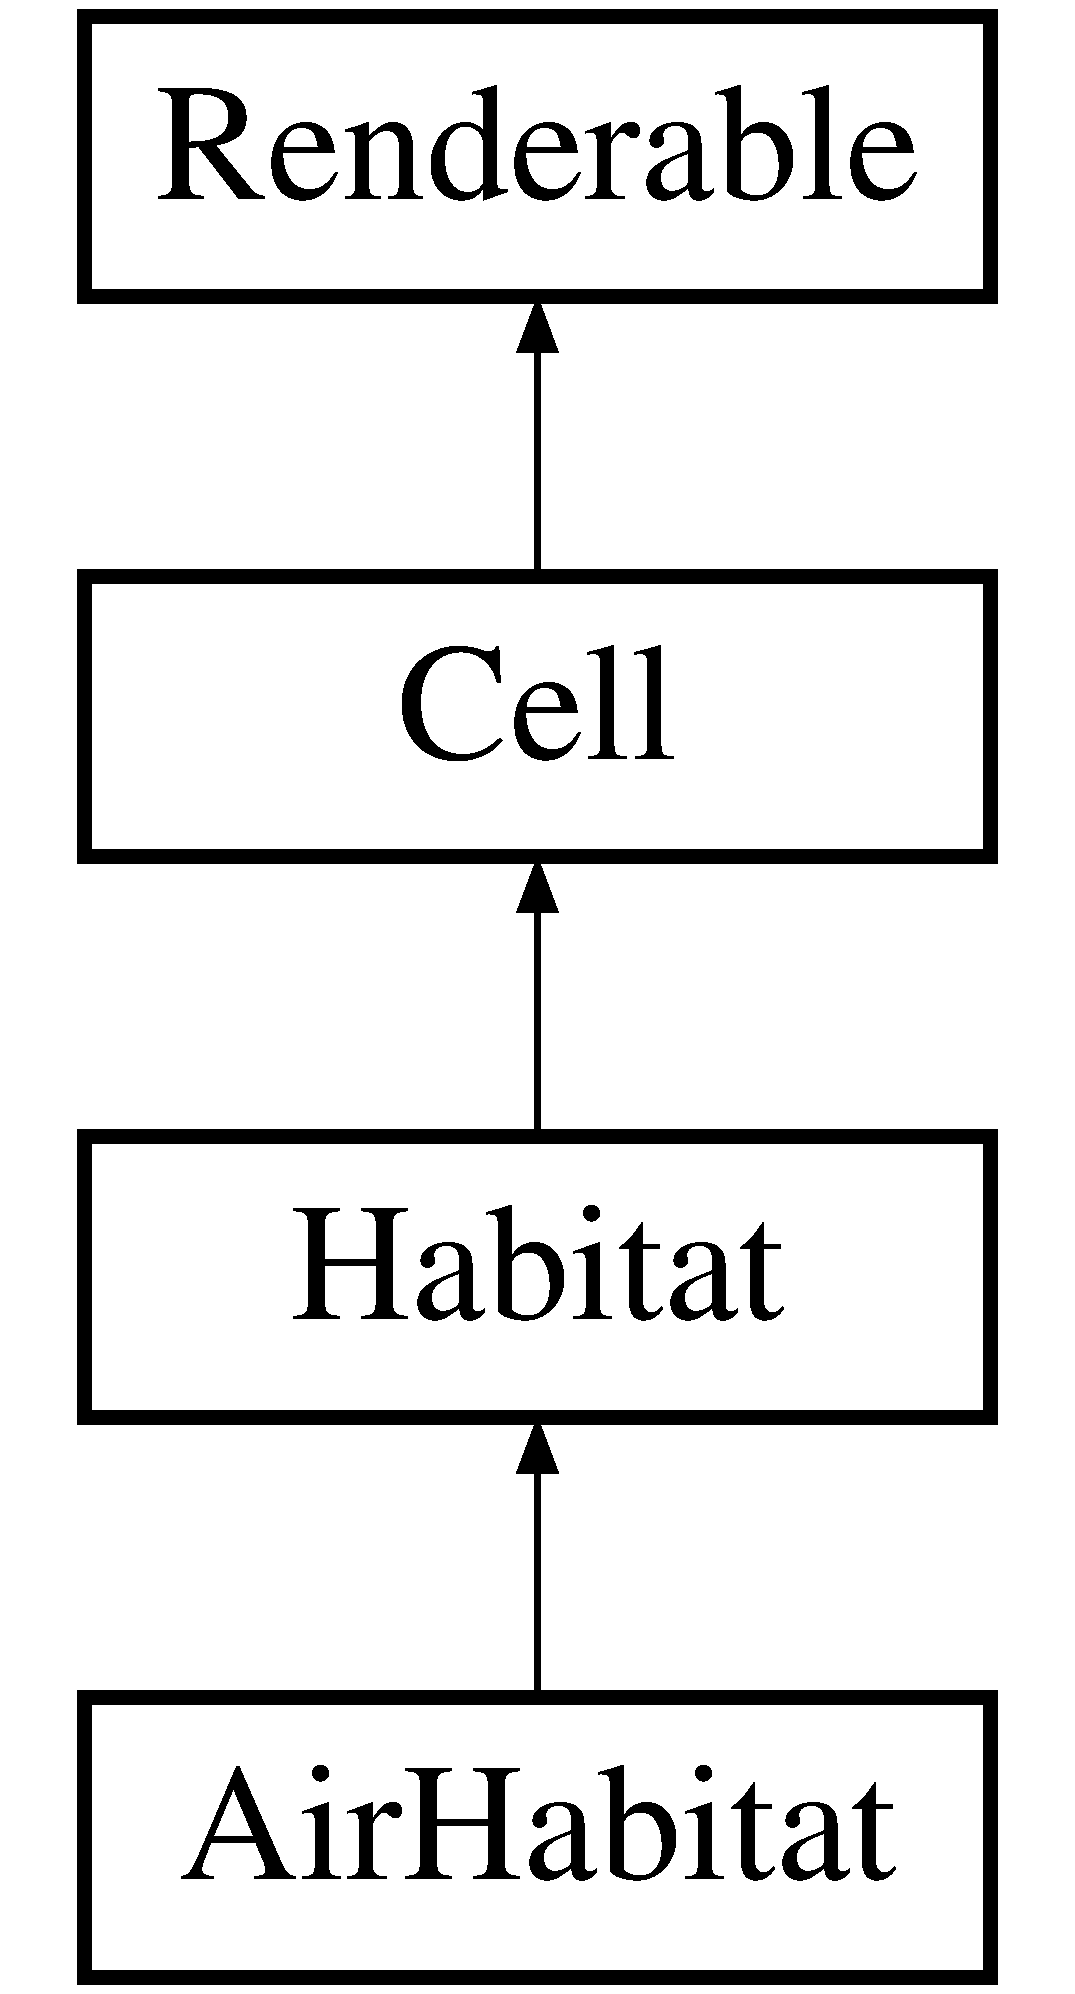
\includegraphics[height=4.000000cm]{classAirHabitat}
\end{center}
\end{figure}
\subsection*{Public Member Functions}
\begin{DoxyCompactItemize}
\item 
\hypertarget{classAirHabitat_aaf82e1201cb35917975fa58ac5a67763}{\hyperlink{classAirHabitat_aaf82e1201cb35917975fa58ac5a67763}{Air\+Habitat} ()}\label{classAirHabitat_aaf82e1201cb35917975fa58ac5a67763}

\begin{DoxyCompactList}\small\item\em Constructor. Menciptakan sebuah \hyperlink{classAirHabitat}{Air\+Habitat}. \end{DoxyCompactList}\item 
\hypertarget{classAirHabitat_a18f98f33d3edbb7c397e184f3b7ad56b}{virtual \hyperlink{classAirHabitat_a18f98f33d3edbb7c397e184f3b7ad56b}{$\sim$\+Air\+Habitat} ()}\label{classAirHabitat_a18f98f33d3edbb7c397e184f3b7ad56b}

\begin{DoxyCompactList}\small\item\em Destructor. \end{DoxyCompactList}\item 
\hypertarget{classAirHabitat_a27885c3ce4486a50629bf1e53cc34905}{void \hyperlink{classAirHabitat_a27885c3ce4486a50629bf1e53cc34905}{render} ()}\label{classAirHabitat_a27885c3ce4486a50629bf1e53cc34905}

\begin{DoxyCompactList}\small\item\em Menampilkan \hyperlink{classAirHabitat}{Air\+Habitat} ke console teks. \end{DoxyCompactList}\end{DoxyCompactItemize}
\subsection*{Additional Inherited Members}


\subsection{Detailed Description}
Kelas \hyperlink{classAirHabitat}{Air\+Habitat} yang merepesentasikan habitat untuk hewan udara. 

The documentation for this class was generated from the following files\+:\begin{DoxyCompactItemize}
\item 
src/\+Cell/\+Habitat/\+Air\+Habitat/Air\+Habitat.\+h\item 
src/\+Cell/\+Habitat/\+Air\+Habitat/Air\+Habitat.\+cpp\end{DoxyCompactItemize}

\hypertarget{classAnimal}{\section{Animal Class Reference}
\label{classAnimal}\index{Animal@{Animal}}
}


{\ttfamily \#include $<$Animal.\+h$>$}

Inheritance diagram for Animal\+:\begin{figure}[H]
\begin{center}
\leavevmode
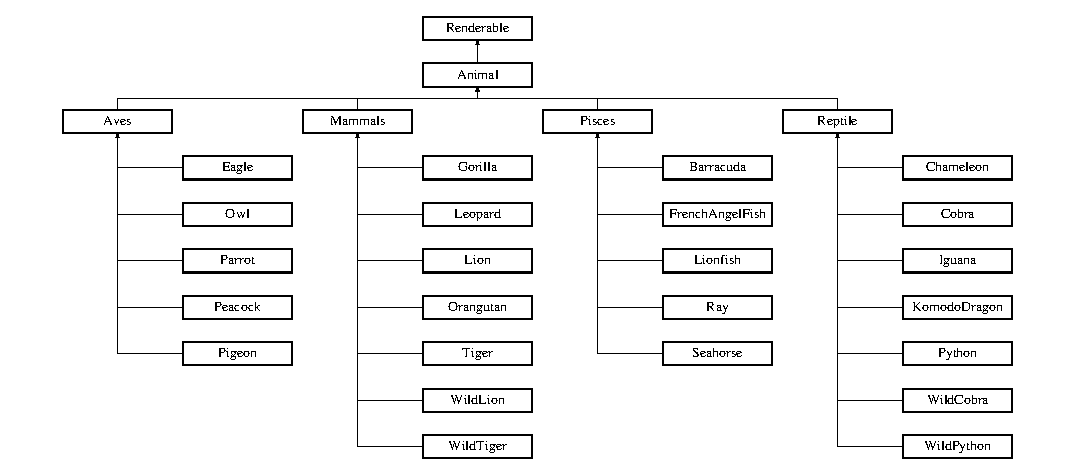
\includegraphics[height=5.932203cm]{classAnimal}
\end{center}
\end{figure}
\subsection*{Public Types}
\begin{DoxyCompactItemize}
\item 
\hypertarget{classAnimal_a5b18980289499046b37cb6973ddd9116}{enum {\bfseries Reproduction} \{ {\bfseries Ovipar}, 
{\bfseries Vivipar}, 
{\bfseries Ovovivipar}
 \}}\label{classAnimal_a5b18980289499046b37cb6973ddd9116}

\item 
\hypertarget{classAnimal_acd95d1fad1f74017e4fc3e1ab6fd2b77}{enum {\bfseries Skin\+Type} \{ {\bfseries Feather}, 
{\bfseries Fur}, 
{\bfseries Scales}
 \}}\label{classAnimal_acd95d1fad1f74017e4fc3e1ab6fd2b77}

\end{DoxyCompactItemize}
\subsection*{Public Member Functions}
\begin{DoxyCompactItemize}
\item 
\hypertarget{classAnimal_a4ef4b49b9ed502193d9a1e447af9dca7}{{\bfseries Animal} (const string \&name)}\label{classAnimal_a4ef4b49b9ed502193d9a1e447af9dca7}

\item 
\hypertarget{classAnimal_a1b2cd74cdd5dee4f3673515bf7672a61}{string {\bfseries get\+Name} () const }\label{classAnimal_a1b2cd74cdd5dee4f3673515bf7672a61}

\item 
\hypertarget{classAnimal_a47dd20676cd213e17556ee4e9d4abe10}{string {\bfseries get\+Description} () const }\label{classAnimal_a47dd20676cd213e17556ee4e9d4abe10}

\item 
bool \hyperlink{classAnimal_a5a672a90eff05c178d324c1f4aced9e1}{is\+Air\+Animal} ()
\begin{DoxyCompactList}\small\item\em Memeriksa apakah hewan adalah hewan udara atau tidak. \end{DoxyCompactList}\item 
bool \hyperlink{classAnimal_a95e08def9cf818b28dc46e63d5073811}{is\+Land\+Animal} ()
\begin{DoxyCompactList}\small\item\em Memeriksa apakah hewan adalah hewan darat atau tidak. \end{DoxyCompactList}\item 
bool \hyperlink{classAnimal_aa70cf2a68c33934d139b129307963494}{is\+Water\+Animal} ()
\begin{DoxyCompactList}\small\item\em Memeriksa apakah hewan adalah hewan air atau tidak. \end{DoxyCompactList}\item 
\hypertarget{classAnimal_a4c613dfd36568f939fc3fa3bdfce4044}{Reproduction {\bfseries get\+Reproduction} () const }\label{classAnimal_a4c613dfd36568f939fc3fa3bdfce4044}

\item 
\hypertarget{classAnimal_a5b2464fd9e2e0153942683f2f84f19de}{Skin\+Type {\bfseries get\+Skin\+Type} () const }\label{classAnimal_a5b2464fd9e2e0153942683f2f84f19de}

\item 
\hypertarget{classAnimal_a2b389702ed4503aae6410eec8c655a40}{\hyperlink{classPoint}{Point} {\bfseries get\+Position} () const }\label{classAnimal_a2b389702ed4503aae6410eec8c655a40}

\item 
\hypertarget{classAnimal_a19098b52e5a13d59a020564c98ab18e9}{void {\bfseries set\+Position} (const \hyperlink{classPoint}{Point} \&position)}\label{classAnimal_a19098b52e5a13d59a020564c98ab18e9}

\item 
virtual string \hyperlink{classAnimal_af2d9616bd719adff241a27bd1ba64725}{interact} ()=0
\begin{DoxyCompactList}\small\item\em Melakukan interaksi dengan seekor hewan. Merupakan pure virtual function. \end{DoxyCompactList}\end{DoxyCompactItemize}
\subsection*{Protected Attributes}
\begin{DoxyCompactItemize}
\item 
\hypertarget{classAnimal_a9cf3bfd9070daec7b3bbc87cbd958f35}{string {\bfseries name}}\label{classAnimal_a9cf3bfd9070daec7b3bbc87cbd958f35}

\item 
\hypertarget{classAnimal_a6662f1a4924469e59b07bab5cdf6e4cb}{Reproduction {\bfseries reproduction}}\label{classAnimal_a6662f1a4924469e59b07bab5cdf6e4cb}

\item 
\hypertarget{classAnimal_a26bf2c81eb76bf25c7d5dc1580270f28}{Skin\+Type {\bfseries skin\+Type}}\label{classAnimal_a26bf2c81eb76bf25c7d5dc1580270f28}

\item 
\hypertarget{classAnimal_a6424e69ec32a75ea293430d4f9e9e30a}{string {\bfseries description}}\label{classAnimal_a6424e69ec32a75ea293430d4f9e9e30a}

\item 
\hypertarget{classAnimal_a38e2249e3bdaf81afa7ca48e11be8630}{bool {\bfseries air\+Animal}}\label{classAnimal_a38e2249e3bdaf81afa7ca48e11be8630}

\item 
\hypertarget{classAnimal_a1a1861bf8610740a24e1cb6dfbd2c06c}{bool {\bfseries land\+Animal}}\label{classAnimal_a1a1861bf8610740a24e1cb6dfbd2c06c}

\item 
\hypertarget{classAnimal_a4f231ab99c669e08504c712bd6676a1d}{bool {\bfseries water\+Animal}}\label{classAnimal_a4f231ab99c669e08504c712bd6676a1d}

\item 
\hypertarget{classAnimal_a2628af9716d1069eb3ddf82b29065214}{\hyperlink{classPoint}{Point} {\bfseries position}}\label{classAnimal_a2628af9716d1069eb3ddf82b29065214}

\end{DoxyCompactItemize}


\subsection{Detailed Description}
Kelas abstrak \hyperlink{classAnimal}{Animal} yang merepesentasikan seekor hewan. 

\subsection{Member Function Documentation}
\hypertarget{classAnimal_af2d9616bd719adff241a27bd1ba64725}{\index{Animal@{Animal}!interact@{interact}}
\index{interact@{interact}!Animal@{Animal}}
\subsubsection[{interact}]{\setlength{\rightskip}{0pt plus 5cm}virtual string Animal\+::interact (
\begin{DoxyParamCaption}
{}
\end{DoxyParamCaption}
)\hspace{0.3cm}{\ttfamily [pure virtual]}}}\label{classAnimal_af2d9616bd719adff241a27bd1ba64725}


Melakukan interaksi dengan seekor hewan. Merupakan pure virtual function. 

\begin{DoxyReturn}{Returns}
string yang menggambarkan experience yang dapat didengar, dirasakan, atau dilihat seorang pengunjung. 
\end{DoxyReturn}
\hypertarget{classAnimal_a5a672a90eff05c178d324c1f4aced9e1}{\index{Animal@{Animal}!is\+Air\+Animal@{is\+Air\+Animal}}
\index{is\+Air\+Animal@{is\+Air\+Animal}!Animal@{Animal}}
\subsubsection[{is\+Air\+Animal}]{\setlength{\rightskip}{0pt plus 5cm}bool Animal\+::is\+Air\+Animal (
\begin{DoxyParamCaption}
{}
\end{DoxyParamCaption}
)}}\label{classAnimal_a5a672a90eff05c178d324c1f4aced9e1}


Memeriksa apakah hewan adalah hewan udara atau tidak. 

\begin{DoxyReturn}{Returns}
True jika hewan adalah hewan udara dan False jika tidak. 
\end{DoxyReturn}
\hypertarget{classAnimal_a95e08def9cf818b28dc46e63d5073811}{\index{Animal@{Animal}!is\+Land\+Animal@{is\+Land\+Animal}}
\index{is\+Land\+Animal@{is\+Land\+Animal}!Animal@{Animal}}
\subsubsection[{is\+Land\+Animal}]{\setlength{\rightskip}{0pt plus 5cm}bool Animal\+::is\+Land\+Animal (
\begin{DoxyParamCaption}
{}
\end{DoxyParamCaption}
)}}\label{classAnimal_a95e08def9cf818b28dc46e63d5073811}


Memeriksa apakah hewan adalah hewan darat atau tidak. 

\begin{DoxyReturn}{Returns}
True jika hewan adalah hewan darat dan False jika tidak. 
\end{DoxyReturn}
\hypertarget{classAnimal_aa70cf2a68c33934d139b129307963494}{\index{Animal@{Animal}!is\+Water\+Animal@{is\+Water\+Animal}}
\index{is\+Water\+Animal@{is\+Water\+Animal}!Animal@{Animal}}
\subsubsection[{is\+Water\+Animal}]{\setlength{\rightskip}{0pt plus 5cm}bool Animal\+::is\+Water\+Animal (
\begin{DoxyParamCaption}
{}
\end{DoxyParamCaption}
)}}\label{classAnimal_aa70cf2a68c33934d139b129307963494}


Memeriksa apakah hewan adalah hewan air atau tidak. 

\begin{DoxyReturn}{Returns}
True jika hewan adalah hewan air dan False jika tidak. 
\end{DoxyReturn}


The documentation for this class was generated from the following files\+:\begin{DoxyCompactItemize}
\item 
src/\+Animal/Animal.\+h\item 
src/\+Animal/Animal.\+cpp\end{DoxyCompactItemize}

\hypertarget{classAves}{\section{Aves Class Reference}
\label{classAves}\index{Aves@{Aves}}
}


{\ttfamily \#include $<$Aves.\+h$>$}

Inheritance diagram for Aves\+:\begin{figure}[H]
\begin{center}
\leavevmode
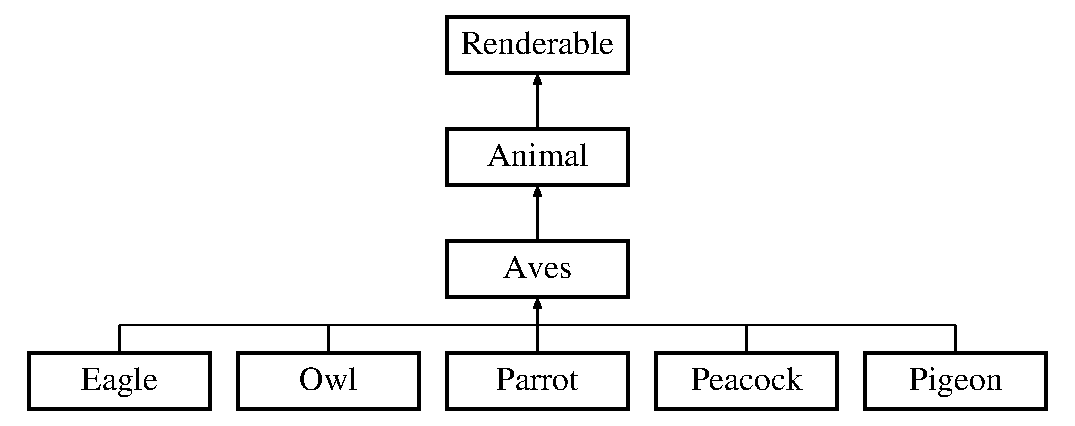
\includegraphics[height=4.000000cm]{classAves}
\end{center}
\end{figure}
\subsection*{Public Member Functions}
\begin{DoxyCompactItemize}
\item 
\hyperlink{classAves_a9594a8bb2bd7576713016b5eaafe7070}{Aves} (const string \&name)
\begin{DoxyCompactList}\small\item\em Constructor. Menciptakan \hyperlink{classAves}{Aves} yang memiliki skin\+Type \char`\"{}\+Feather\char`\"{} dan reproduction \char`\"{}\+Ovipar\char`\"{}. \end{DoxyCompactList}\end{DoxyCompactItemize}
\subsection*{Additional Inherited Members}


\subsection{Detailed Description}
Kelas abstrak \hyperlink{classAves}{Aves} yang merepesentasikan kelas hewan \hyperlink{classAves}{Aves}. 

\subsection{Constructor \& Destructor Documentation}
\hypertarget{classAves_a9594a8bb2bd7576713016b5eaafe7070}{\index{Aves@{Aves}!Aves@{Aves}}
\index{Aves@{Aves}!Aves@{Aves}}
\subsubsection[{Aves}]{\setlength{\rightskip}{0pt plus 5cm}Aves\+::\+Aves (
\begin{DoxyParamCaption}
\item[{const string \&}]{name}
\end{DoxyParamCaption}
)}}\label{classAves_a9594a8bb2bd7576713016b5eaafe7070}


Constructor. Menciptakan \hyperlink{classAves}{Aves} yang memiliki skin\+Type \char`\"{}\+Feather\char`\"{} dan reproduction \char`\"{}\+Ovipar\char`\"{}. 


\begin{DoxyParams}{Parameters}
{\em name} & Nama hewan \\
\hline
\end{DoxyParams}


The documentation for this class was generated from the following files\+:\begin{DoxyCompactItemize}
\item 
src/\+Animal/\+Aves/Aves.\+h\item 
src/\+Animal/\+Aves/Aves.\+cpp\end{DoxyCompactItemize}

\hypertarget{classBarracuda}{\section{Barracuda Class Reference}
\label{classBarracuda}\index{Barracuda@{Barracuda}}
}


{\ttfamily \#include $<$Barracuda.\+h$>$}

Inheritance diagram for Barracuda\+:\begin{figure}[H]
\begin{center}
\leavevmode
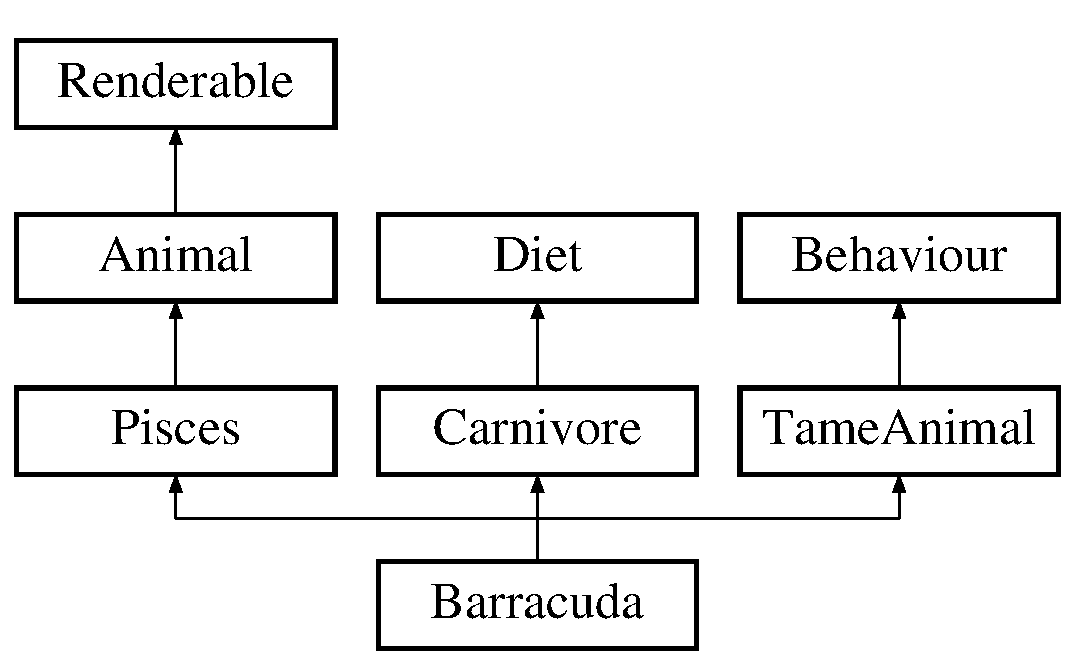
\includegraphics[height=4.000000cm]{classBarracuda}
\end{center}
\end{figure}
\subsection*{Public Member Functions}
\begin{DoxyCompactItemize}
\item 
\hypertarget{classBarracuda_af12ecb7d4914ab078da251f702cfb2bf}{\hyperlink{classBarracuda_af12ecb7d4914ab078da251f702cfb2bf}{Barracuda} (int \+\_\+weight)}\label{classBarracuda_af12ecb7d4914ab078da251f702cfb2bf}

\begin{DoxyCompactList}\small\item\em Constructor. Menciptakan ikan barakuda. \end{DoxyCompactList}\item 
string \hyperlink{classBarracuda_aceb93a0bb776083679e70965159e17bc}{interact} () const 
\begin{DoxyCompactList}\small\item\em Melakukan interaksi dengan ikan barakuda. \end{DoxyCompactList}\end{DoxyCompactItemize}
\subsection*{Additional Inherited Members}


\subsection{Detailed Description}
Kelas \hyperlink{classBarracuda}{Barracuda} yang merepesentasikan ikan barakuda. 

\subsection{Member Function Documentation}
\hypertarget{classBarracuda_aceb93a0bb776083679e70965159e17bc}{\index{Barracuda@{Barracuda}!interact@{interact}}
\index{interact@{interact}!Barracuda@{Barracuda}}
\subsubsection[{interact}]{\setlength{\rightskip}{0pt plus 5cm}string Barracuda\+::interact (
\begin{DoxyParamCaption}
{}
\end{DoxyParamCaption}
) const}}\label{classBarracuda_aceb93a0bb776083679e70965159e17bc}


Melakukan interaksi dengan ikan barakuda. 

\begin{DoxyReturn}{Returns}
Experience yang dirasakan ketika berinteraksi dengan ikan barakuda. 
\end{DoxyReturn}


The documentation for this class was generated from the following files\+:\begin{DoxyCompactItemize}
\item 
src/\+Animal/\+Pisces/\+Barracuda/Barracuda.\+h\item 
src/\+Animal/\+Pisces/\+Barracuda/Barracuda.\+cpp\end{DoxyCompactItemize}

\hypertarget{classBehaviour}{\section{Behaviour Class Reference}
\label{classBehaviour}\index{Behaviour@{Behaviour}}
}
Inheritance diagram for Behaviour\+:\begin{figure}[H]
\begin{center}
\leavevmode
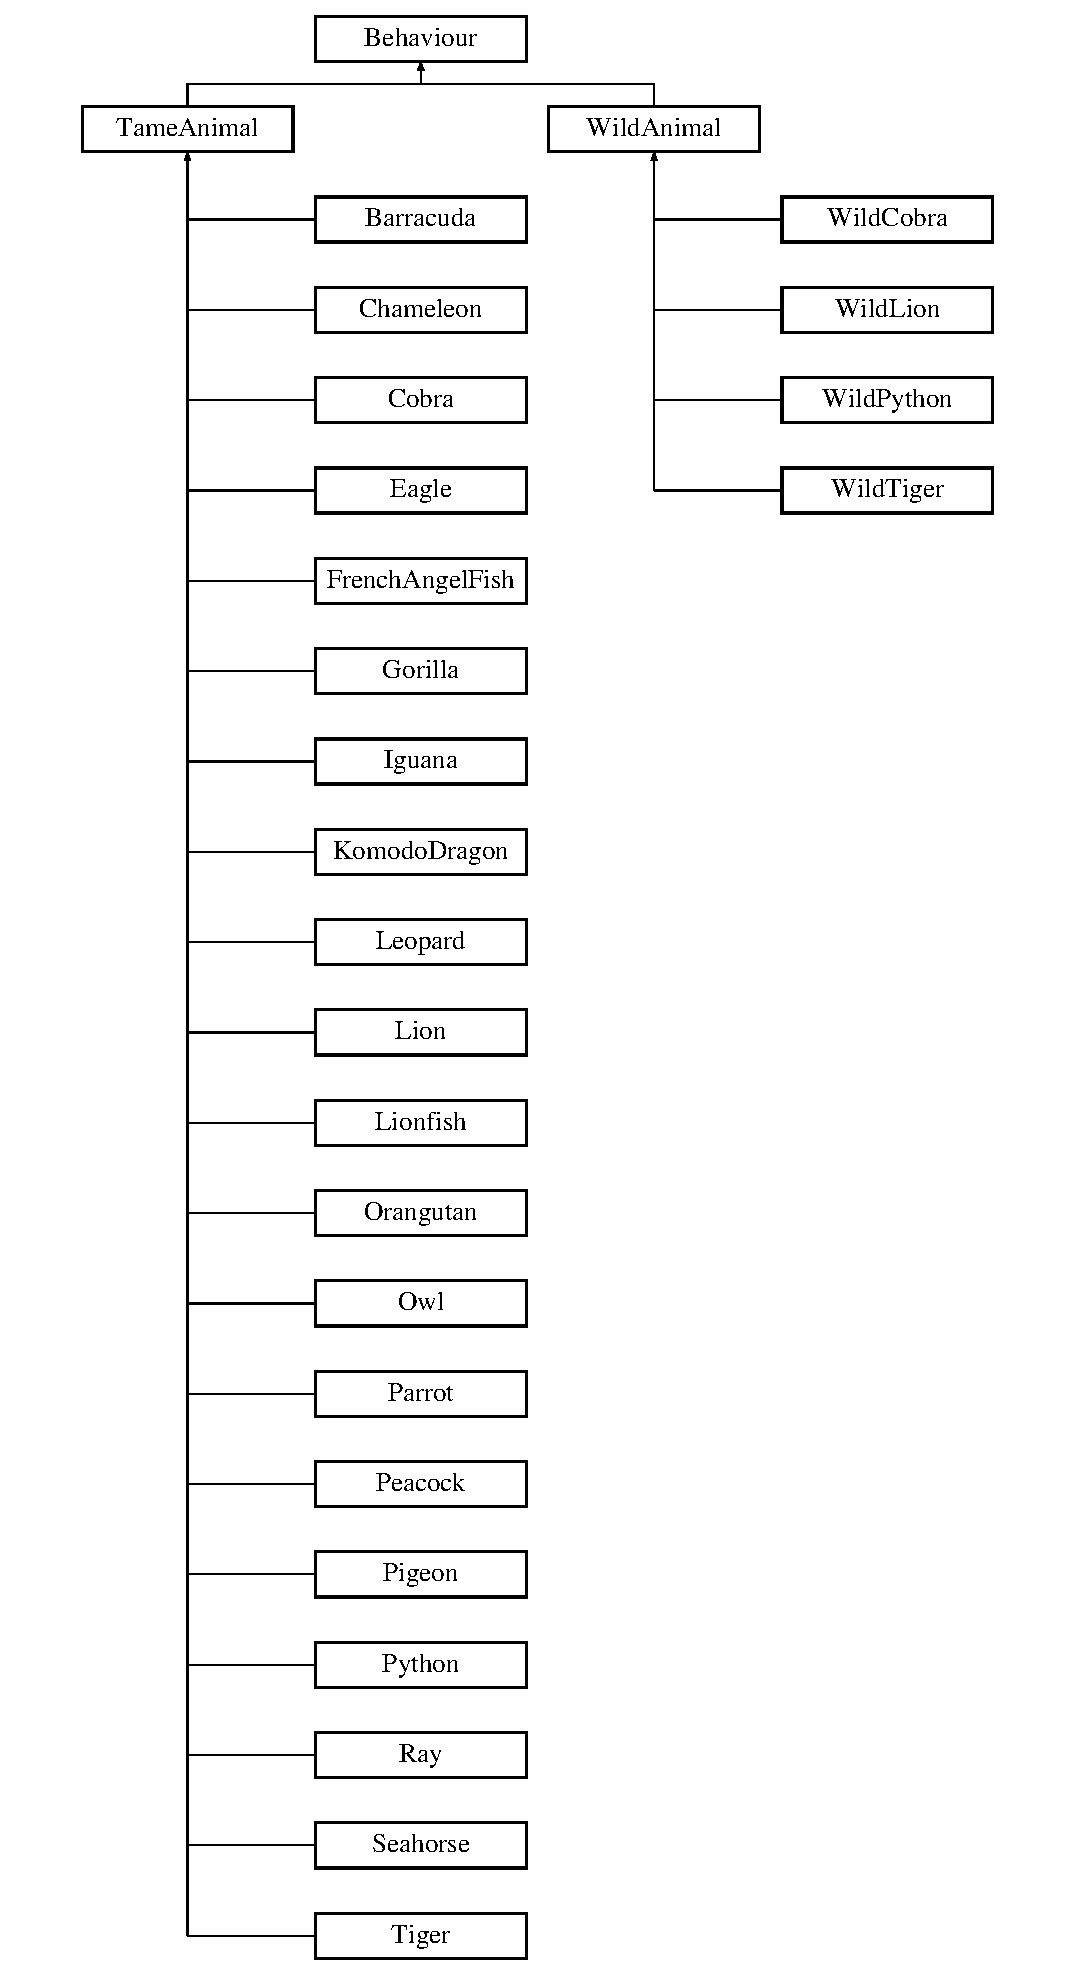
\includegraphics[height=12.000000cm]{classBehaviour}
\end{center}
\end{figure}
\subsection*{Classes}
\begin{DoxyCompactItemize}
\item 
class \hyperlink{classBehaviour_1_1Kelas}{Kelas}
\end{DoxyCompactItemize}
\subsection*{Public Member Functions}
\begin{DoxyCompactItemize}
\item 
\hyperlink{classBehaviour_ac4cb25471318a26c5bbf32d5434fcb2a}{Behaviour} (bool \+\_\+wild)
\item 
\hypertarget{classBehaviour_a7b616730b27f966b6f8d747297ee3028}{virtual \hyperlink{classBehaviour_a7b616730b27f966b6f8d747297ee3028}{$\sim$\+Behaviour} ()}\label{classBehaviour_a7b616730b27f966b6f8d747297ee3028}

\begin{DoxyCompactList}\small\item\em Destructor. \end{DoxyCompactList}\item 
bool \hyperlink{classBehaviour_a794dd5abfc1f207dc36ee634f4eb9a89}{is\+Wild} () const 
\begin{DoxyCompactList}\small\item\em Memeriksa apakah hewan buas atau tidak. \end{DoxyCompactList}\end{DoxyCompactItemize}
\subsection*{Protected Attributes}
\begin{DoxyCompactItemize}
\item 
\hypertarget{classBehaviour_a1878148bf558dfb84dc9ff6be180cc01}{bool {\bfseries wild}}\label{classBehaviour_a1878148bf558dfb84dc9ff6be180cc01}

\end{DoxyCompactItemize}


\subsection{Constructor \& Destructor Documentation}
\hypertarget{classBehaviour_ac4cb25471318a26c5bbf32d5434fcb2a}{\index{Behaviour@{Behaviour}!Behaviour@{Behaviour}}
\index{Behaviour@{Behaviour}!Behaviour@{Behaviour}}
\subsubsection[{Behaviour}]{\setlength{\rightskip}{0pt plus 5cm}Behaviour\+::\+Behaviour (
\begin{DoxyParamCaption}
\item[{bool}]{\+\_\+wild}
\end{DoxyParamCaption}
)}}\label{classBehaviour_ac4cb25471318a26c5bbf32d5434fcb2a}
. Menciptakan hewan dengan kelakuan tertentu (buas atau jinak). 
\begin{DoxyParams}{Parameters}
{\em \+\_\+wild} & Kelakuan hewan (True jika liar dan false jika tidak). \\
\hline
\end{DoxyParams}


\subsection{Member Function Documentation}
\hypertarget{classBehaviour_a794dd5abfc1f207dc36ee634f4eb9a89}{\index{Behaviour@{Behaviour}!is\+Wild@{is\+Wild}}
\index{is\+Wild@{is\+Wild}!Behaviour@{Behaviour}}
\subsubsection[{is\+Wild}]{\setlength{\rightskip}{0pt plus 5cm}bool Behaviour\+::is\+Wild (
\begin{DoxyParamCaption}
{}
\end{DoxyParamCaption}
) const}}\label{classBehaviour_a794dd5abfc1f207dc36ee634f4eb9a89}


Memeriksa apakah hewan buas atau tidak. 

\begin{DoxyReturn}{Returns}
True jika hewan adalah hewan buas dan False jika tidak. 
\end{DoxyReturn}


The documentation for this class was generated from the following file\+:\begin{DoxyCompactItemize}
\item 
src/\+Animal/\+Behaviour/Behaviour.\+h\end{DoxyCompactItemize}

\hypertarget{classCage}{\section{Cage Class Reference}
\label{classCage}\index{Cage@{Cage}}
}


{\ttfamily \#include $<$Cage.\+h$>$}

Inheritance diagram for Cage\+:\begin{figure}[H]
\begin{center}
\leavevmode
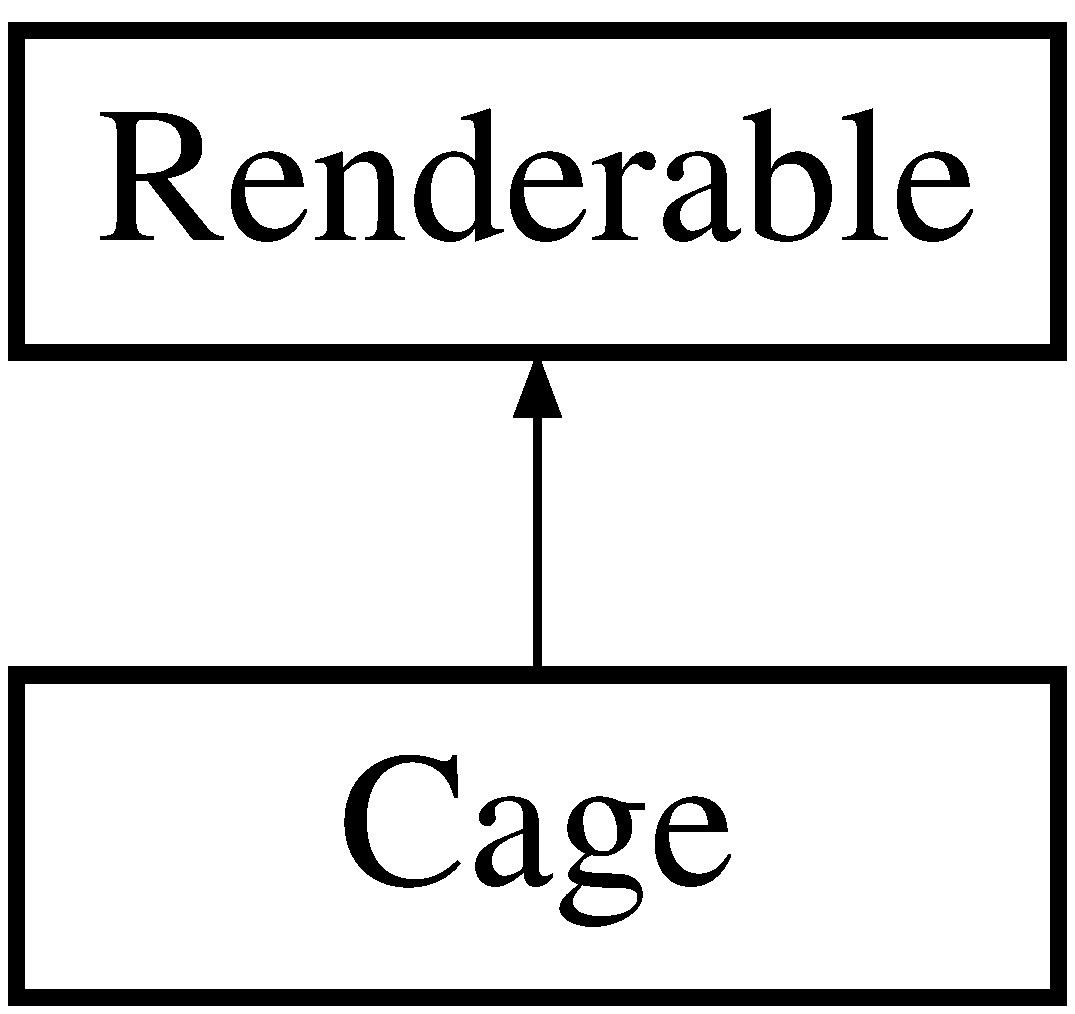
\includegraphics[height=2.000000cm]{classCage}
\end{center}
\end{figure}
\subsection*{Public Member Functions}
\begin{DoxyCompactItemize}
\item 
\hyperlink{classCage_a9010aec97e645b7a5374ef02129b7dc3}{Cage} (int \+\_\+size)
\begin{DoxyCompactList}\small\item\em Constructor. Menciptakan sebuah kandang dengan ukuran tertentu dengan jumlah kapasitas hewan maksimal 30\% dari ukuran kandang. Jumlah hewan di dalam kandang diinisialisasi dengan nol. \end{DoxyCompactList}\item 
\hypertarget{classCage_a657259499dfc23c63fc65aeaf8abbb17}{\hyperlink{classCage_a657259499dfc23c63fc65aeaf8abbb17}{$\sim$\+Cage} ()}\label{classCage_a657259499dfc23c63fc65aeaf8abbb17}

\begin{DoxyCompactList}\small\item\em Destructor. \end{DoxyCompactList}\item 
void \hyperlink{classCage_a3315b5b1e578b9a57bd52b7bd84851eb}{add\+Animal} (\hyperlink{classAnimal}{Animal} $\ast$\+\_\+animal)
\begin{DoxyCompactList}\small\item\em Menambahkan seekor hewan ke dalam kandang. Kandang tidak berada dalam keaddan penuh. \end{DoxyCompactList}\item 
void \hyperlink{classCage_adc760f475c13edb5e4f34606ca211e6a}{add\+Habitat} (\hyperlink{classHabitat}{Habitat} $\ast$\+\_\+habitat)
\begin{DoxyCompactList}\small\item\em Menambahkan sebuah habitat ke dalam kandang. \end{DoxyCompactList}\item 
bool \hyperlink{classCage_a6e4f2417918ef61eee36cdf27a807a8d}{is\+Full} () const 
\begin{DoxyCompactList}\small\item\em Memeriksa apakah jumlah hewan di dalam kandang sudah mencapai kapasitas atau belum. \end{DoxyCompactList}\item 
\hypertarget{classCage_a42eda8d1a0f6b5105a0c5dfc75cebe70}{void \hyperlink{classCage_a42eda8d1a0f6b5105a0c5dfc75cebe70}{render} ()}\label{classCage_a42eda8d1a0f6b5105a0c5dfc75cebe70}

\begin{DoxyCompactList}\small\item\em Menampilkan kandang ke console teks. \end{DoxyCompactList}\end{DoxyCompactItemize}


\subsection{Detailed Description}
Kelas \hyperlink{classCage}{Cage} yang merepesentasikan kandang. 

\subsection{Constructor \& Destructor Documentation}
\hypertarget{classCage_a9010aec97e645b7a5374ef02129b7dc3}{\index{Cage@{Cage}!Cage@{Cage}}
\index{Cage@{Cage}!Cage@{Cage}}
\subsubsection[{Cage}]{\setlength{\rightskip}{0pt plus 5cm}Cage\+::\+Cage (
\begin{DoxyParamCaption}
\item[{int}]{\+\_\+size}
\end{DoxyParamCaption}
)}}\label{classCage_a9010aec97e645b7a5374ef02129b7dc3}


Constructor. Menciptakan sebuah kandang dengan ukuran tertentu dengan jumlah kapasitas hewan maksimal 30\% dari ukuran kandang. Jumlah hewan di dalam kandang diinisialisasi dengan nol. 


\begin{DoxyParams}{Parameters}
{\em \+\_\+size} & Nilai ukuran kandang. \\
\hline
\end{DoxyParams}


\subsection{Member Function Documentation}
\hypertarget{classCage_a3315b5b1e578b9a57bd52b7bd84851eb}{\index{Cage@{Cage}!add\+Animal@{add\+Animal}}
\index{add\+Animal@{add\+Animal}!Cage@{Cage}}
\subsubsection[{add\+Animal}]{\setlength{\rightskip}{0pt plus 5cm}void Cage\+::add\+Animal (
\begin{DoxyParamCaption}
\item[{{\bf Animal} $\ast$}]{\+\_\+animal}
\end{DoxyParamCaption}
)}}\label{classCage_a3315b5b1e578b9a57bd52b7bd84851eb}


Menambahkan seekor hewan ke dalam kandang. Kandang tidak berada dalam keaddan penuh. 


\begin{DoxyParams}{Parameters}
{\em \+\_\+animal} & Hewan yang dimasukkan ke dalam kandang. \\
\hline
\end{DoxyParams}
\hypertarget{classCage_adc760f475c13edb5e4f34606ca211e6a}{\index{Cage@{Cage}!add\+Habitat@{add\+Habitat}}
\index{add\+Habitat@{add\+Habitat}!Cage@{Cage}}
\subsubsection[{add\+Habitat}]{\setlength{\rightskip}{0pt plus 5cm}void Cage\+::add\+Habitat (
\begin{DoxyParamCaption}
\item[{{\bf Habitat} $\ast$}]{\+\_\+habitat}
\end{DoxyParamCaption}
)}}\label{classCage_adc760f475c13edb5e4f34606ca211e6a}


Menambahkan sebuah habitat ke dalam kandang. 


\begin{DoxyParams}{Parameters}
{\em \+\_\+habitat} & \hyperlink{classHabitat}{Habitat} yang berada di dalam kandang. \\
\hline
\end{DoxyParams}
\hypertarget{classCage_a6e4f2417918ef61eee36cdf27a807a8d}{\index{Cage@{Cage}!is\+Full@{is\+Full}}
\index{is\+Full@{is\+Full}!Cage@{Cage}}
\subsubsection[{is\+Full}]{\setlength{\rightskip}{0pt plus 5cm}bool Cage\+::is\+Full (
\begin{DoxyParamCaption}
{}
\end{DoxyParamCaption}
) const}}\label{classCage_a6e4f2417918ef61eee36cdf27a807a8d}


Memeriksa apakah jumlah hewan di dalam kandang sudah mencapai kapasitas atau belum. 

\begin{DoxyReturn}{Returns}
True jika jumlah hewan sudah mencapai kapasitas kandang dan false jika belum. 
\end{DoxyReturn}


The documentation for this class was generated from the following file\+:\begin{DoxyCompactItemize}
\item 
src/\+Cage/Cage.\+h\end{DoxyCompactItemize}

\hypertarget{classCarnivore}{\section{Carnivore Class Reference}
\label{classCarnivore}\index{Carnivore@{Carnivore}}
}
Inheritance diagram for Carnivore\+:\begin{figure}[H]
\begin{center}
\leavevmode
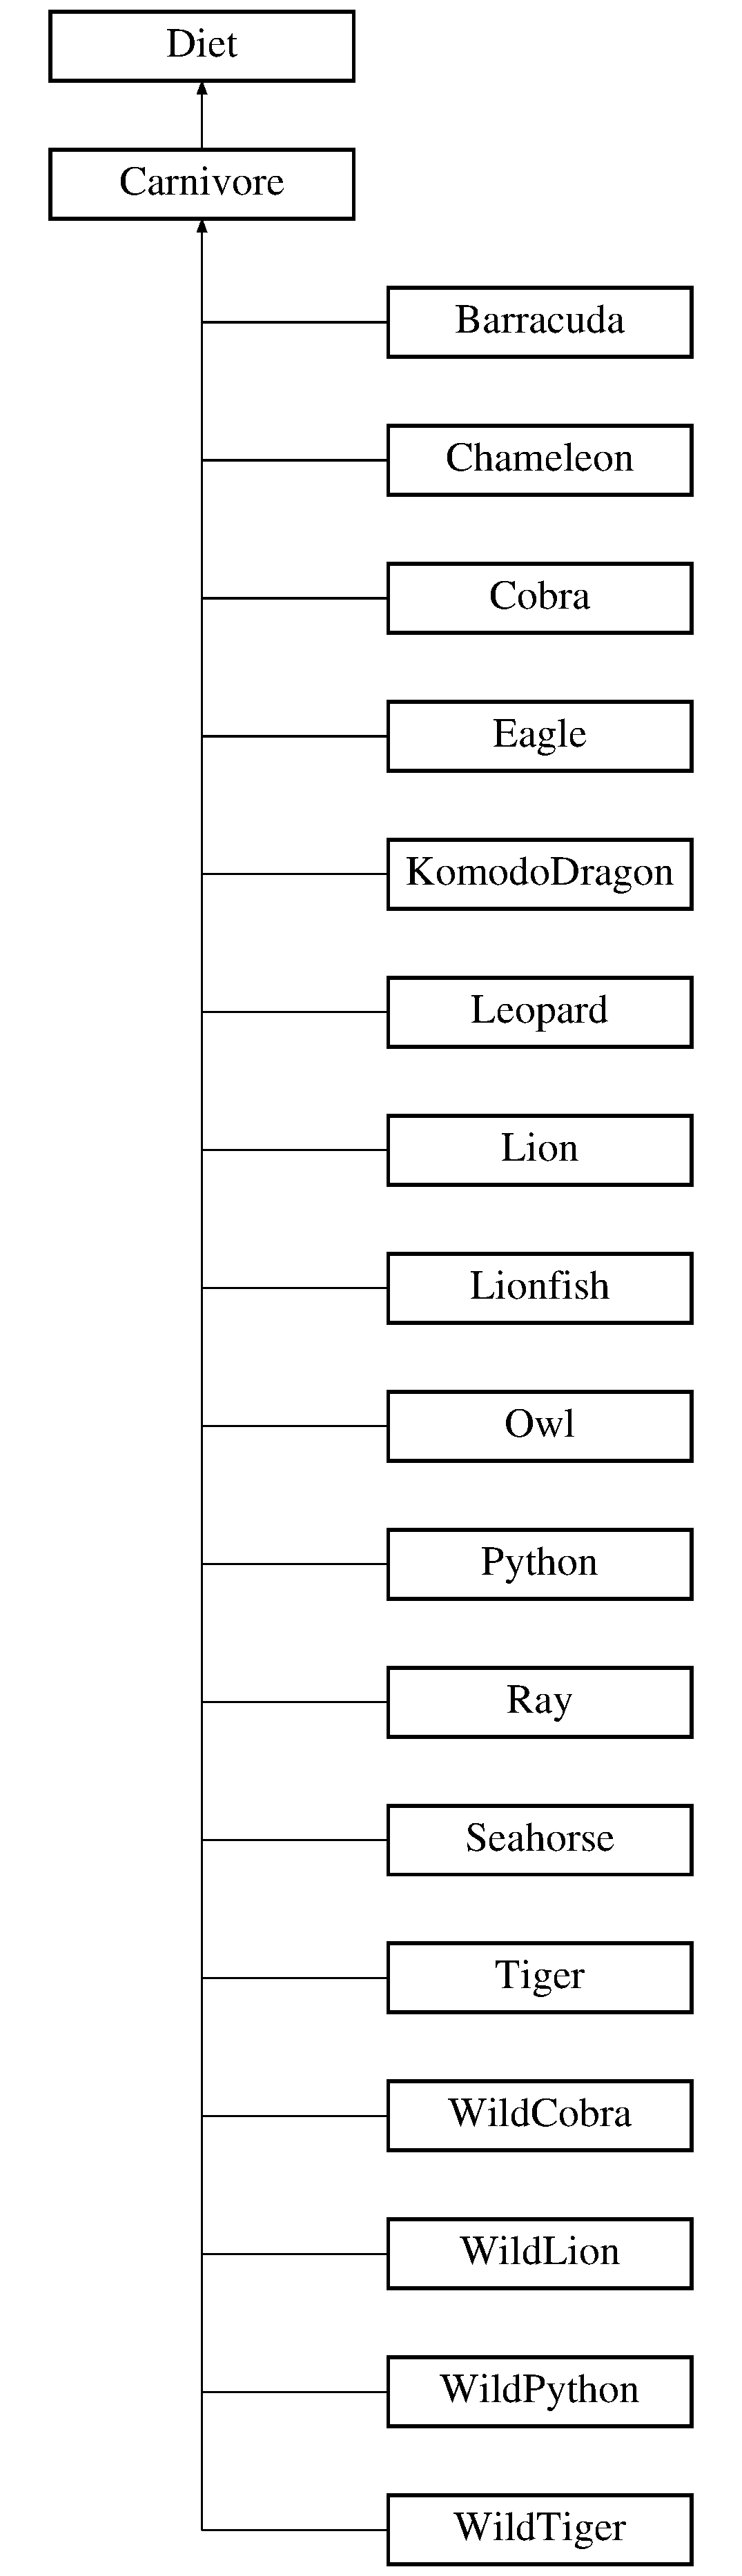
\includegraphics[height=12.000000cm]{classCarnivore}
\end{center}
\end{figure}
\subsection*{Public Member Functions}
\begin{DoxyCompactItemize}
\item 
\hyperlink{classCarnivore_a5c6829c7909ecb4a280a2c9652ce58a4}{Carnivore} (int \+\_\+weight, double \+\_\+ratio)
\begin{DoxyCompactList}\small\item\em Constructor. Menciptakan hewan karnivora dengan berat tertentu. \end{DoxyCompactList}\end{DoxyCompactItemize}
\subsection*{Additional Inherited Members}


\subsection{Constructor \& Destructor Documentation}
\hypertarget{classCarnivore_a5c6829c7909ecb4a280a2c9652ce58a4}{\index{Carnivore@{Carnivore}!Carnivore@{Carnivore}}
\index{Carnivore@{Carnivore}!Carnivore@{Carnivore}}
\subsubsection[{Carnivore}]{\setlength{\rightskip}{0pt plus 5cm}Carnivore\+::\+Carnivore (
\begin{DoxyParamCaption}
\item[{int}]{\+\_\+weight, }
\item[{double}]{\+\_\+ratio}
\end{DoxyParamCaption}
)}}\label{classCarnivore_a5c6829c7909ecb4a280a2c9652ce58a4}


Constructor. Menciptakan hewan karnivora dengan berat tertentu. 


\begin{DoxyParams}{Parameters}
{\em \+\_\+weight} & Berat dari hewan. \\
\hline
\end{DoxyParams}


The documentation for this class was generated from the following files\+:\begin{DoxyCompactItemize}
\item 
src/\+Animal/\+Diet/\+Carnivore/Carnivore.\+h\item 
src/\+Animal/\+Diet/\+Carnivore/Carnivore.\+cpp\end{DoxyCompactItemize}

\hypertarget{classCell}{\section{Cell Class Reference}
\label{classCell}\index{Cell@{Cell}}
}


{\ttfamily \#include $<$Cell.\+h$>$}

Inheritance diagram for Cell\+:\begin{figure}[H]
\begin{center}
\leavevmode
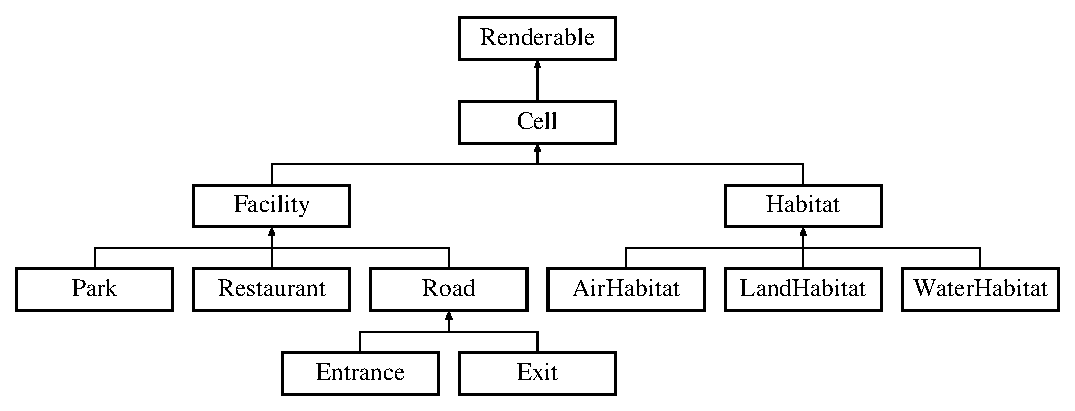
\includegraphics[height=5.000000cm]{classCell}
\end{center}
\end{figure}
\subsection*{Public Member Functions}
\begin{DoxyCompactItemize}
\item 
\hyperlink{classCell_a38aede1bc2a5d27ee327109c1cb646ab}{Cell} (bool \+\_\+accessible)
\begin{DoxyCompactList}\small\item\em Constructor. Menciptakan sebuah \hyperlink{classCell}{Cell} dengan status aksesibilitas tertentu. \end{DoxyCompactList}\item 
\hypertarget{classCell_a9fa559f7a28e2b4336c6879ca09304d8}{virtual \hyperlink{classCell_a9fa559f7a28e2b4336c6879ca09304d8}{$\sim$\+Cell} ()}\label{classCell_a9fa559f7a28e2b4336c6879ca09304d8}

\begin{DoxyCompactList}\small\item\em Destructor. \end{DoxyCompactList}\item 
bool \hyperlink{classCell_aef7a11f9388d041cebb90d15ab2890ad}{is\+Accessible} () const 
\begin{DoxyCompactList}\small\item\em Memeriksa status aksesibilitas dari \hyperlink{classCell}{Cell}. \end{DoxyCompactList}\item 
void \hyperlink{classCell_a53dfa4264f46ca0a8c65004731793aa9}{set\+Position} (const \hyperlink{classPoint}{Point} \&\+\_\+position)
\begin{DoxyCompactList}\small\item\em Menset posisi dari \hyperlink{classCell}{Cell}. \end{DoxyCompactList}\item 
int \hyperlink{classCell_a78d82b277e8fb2e1c3e70286bcc85314}{get\+X} () const 
\begin{DoxyCompactList}\small\item\em Mengambil nilai absis dari posisi \hyperlink{classCell}{Cell}. \end{DoxyCompactList}\item 
int \hyperlink{classCell_a2df3d69f5d0c10a1e1f02c5f89045e0a}{get\+Y} () const 
\begin{DoxyCompactList}\small\item\em Mengambil nilai ordinat dari posisi \hyperlink{classCell}{Cell}. \end{DoxyCompactList}\end{DoxyCompactItemize}
\subsection*{Protected Attributes}
\begin{DoxyCompactItemize}
\item 
\hypertarget{classCell_a4c07dcb183072ac6fa92b3414a02b26b}{const bool {\bfseries accessible}}\label{classCell_a4c07dcb183072ac6fa92b3414a02b26b}

\item 
\hypertarget{classCell_a95e83c73197426f8da1b62809c00041e}{\hyperlink{classPoint}{Point} {\bfseries position}}\label{classCell_a95e83c73197426f8da1b62809c00041e}

\end{DoxyCompactItemize}


\subsection{Detailed Description}
Kelas abstrak \hyperlink{classCell}{Cell} yang merepesentasikan petak tanah berukuran 1m x 1m. 

\subsection{Constructor \& Destructor Documentation}
\hypertarget{classCell_a38aede1bc2a5d27ee327109c1cb646ab}{\index{Cell@{Cell}!Cell@{Cell}}
\index{Cell@{Cell}!Cell@{Cell}}
\subsubsection[{Cell}]{\setlength{\rightskip}{0pt plus 5cm}Cell\+::\+Cell (
\begin{DoxyParamCaption}
\item[{bool}]{\+\_\+accessible}
\end{DoxyParamCaption}
)}}\label{classCell_a38aede1bc2a5d27ee327109c1cb646ab}


Constructor. Menciptakan sebuah \hyperlink{classCell}{Cell} dengan status aksesibilitas tertentu. 


\begin{DoxyParams}{Parameters}
{\em \+\_\+accessible} & Status aksesibilitas dari \hyperlink{classCell}{Cell}. \\
\hline
\end{DoxyParams}


\subsection{Member Function Documentation}
\hypertarget{classCell_a78d82b277e8fb2e1c3e70286bcc85314}{\index{Cell@{Cell}!get\+X@{get\+X}}
\index{get\+X@{get\+X}!Cell@{Cell}}
\subsubsection[{get\+X}]{\setlength{\rightskip}{0pt plus 5cm}int Cell\+::get\+X (
\begin{DoxyParamCaption}
{}
\end{DoxyParamCaption}
) const\hspace{0.3cm}{\ttfamily [virtual]}}}\label{classCell_a78d82b277e8fb2e1c3e70286bcc85314}


Mengambil nilai absis dari posisi \hyperlink{classCell}{Cell}. 

\begin{DoxyReturn}{Returns}
Nilai absis dari posisi \hyperlink{classCell}{Cell}. 
\end{DoxyReturn}


Implements \hyperlink{classRenderable_af0e3e758db2aad1d0d874fc98736614f}{Renderable}.

\hypertarget{classCell_a2df3d69f5d0c10a1e1f02c5f89045e0a}{\index{Cell@{Cell}!get\+Y@{get\+Y}}
\index{get\+Y@{get\+Y}!Cell@{Cell}}
\subsubsection[{get\+Y}]{\setlength{\rightskip}{0pt plus 5cm}int Cell\+::get\+Y (
\begin{DoxyParamCaption}
{}
\end{DoxyParamCaption}
) const\hspace{0.3cm}{\ttfamily [virtual]}}}\label{classCell_a2df3d69f5d0c10a1e1f02c5f89045e0a}


Mengambil nilai ordinat dari posisi \hyperlink{classCell}{Cell}. 

\begin{DoxyReturn}{Returns}
Nilai ordinat dari posisi \hyperlink{classCell}{Cell}. 
\end{DoxyReturn}


Implements \hyperlink{classRenderable_a6af0fc98ab82083dce18e9ea970480e0}{Renderable}.

\hypertarget{classCell_aef7a11f9388d041cebb90d15ab2890ad}{\index{Cell@{Cell}!is\+Accessible@{is\+Accessible}}
\index{is\+Accessible@{is\+Accessible}!Cell@{Cell}}
\subsubsection[{is\+Accessible}]{\setlength{\rightskip}{0pt plus 5cm}bool Cell\+::is\+Accessible (
\begin{DoxyParamCaption}
{}
\end{DoxyParamCaption}
) const}}\label{classCell_aef7a11f9388d041cebb90d15ab2890ad}


Memeriksa status aksesibilitas dari \hyperlink{classCell}{Cell}. 

\begin{DoxyReturn}{Returns}
Status aksesibiltas dari \hyperlink{classCell}{Cell} (true jika bisa diakses dan false jika tidak). 
\end{DoxyReturn}
\hypertarget{classCell_a53dfa4264f46ca0a8c65004731793aa9}{\index{Cell@{Cell}!set\+Position@{set\+Position}}
\index{set\+Position@{set\+Position}!Cell@{Cell}}
\subsubsection[{set\+Position}]{\setlength{\rightskip}{0pt plus 5cm}void Cell\+::set\+Position (
\begin{DoxyParamCaption}
\item[{const {\bf Point} \&}]{\+\_\+position}
\end{DoxyParamCaption}
)}}\label{classCell_a53dfa4264f46ca0a8c65004731793aa9}


Menset posisi dari \hyperlink{classCell}{Cell}. 


\begin{DoxyParams}{Parameters}
{\em \+\_\+position} & Posisi dari \hyperlink{classCell}{Cell}. \\
\hline
\end{DoxyParams}


The documentation for this class was generated from the following files\+:\begin{DoxyCompactItemize}
\item 
src/\+Cell/Cell.\+h\item 
src/\+Cell/Cell.\+cpp\end{DoxyCompactItemize}

\hypertarget{classChameleon}{\section{Chameleon Class Reference}
\label{classChameleon}\index{Chameleon@{Chameleon}}
}


{\ttfamily \#include $<$Chameleon.\+h$>$}

Inheritance diagram for Chameleon\+:\begin{figure}[H]
\begin{center}
\leavevmode
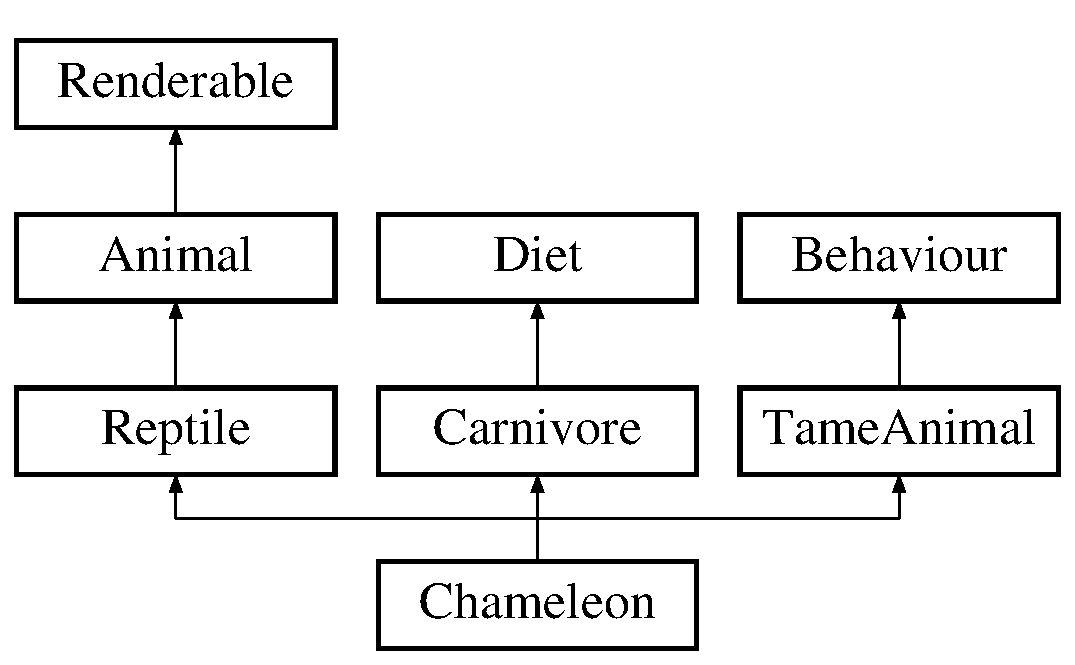
\includegraphics[height=4.000000cm]{classChameleon}
\end{center}
\end{figure}
\subsection*{Public Member Functions}
\begin{DoxyCompactItemize}
\item 
\hypertarget{classChameleon_a964d02d53c3f97e72b4331a443b9a8ab}{\hyperlink{classChameleon_a964d02d53c3f97e72b4331a443b9a8ab}{Chameleon} (int \+\_\+weight)}\label{classChameleon_a964d02d53c3f97e72b4331a443b9a8ab}

\begin{DoxyCompactList}\small\item\em Constructor. Menciptakan bunglon. \end{DoxyCompactList}\item 
string \hyperlink{classChameleon_af2d7cd98b862a6c93a757a43c701f74f}{interact} () const 
\begin{DoxyCompactList}\small\item\em Melakukan interaksi dengan bunglon. \end{DoxyCompactList}\end{DoxyCompactItemize}
\subsection*{Additional Inherited Members}


\subsection{Detailed Description}
Kelas \hyperlink{classChameleon}{Chameleon} yang merepesentasikan bunglon. 

\subsection{Member Function Documentation}
\hypertarget{classChameleon_af2d7cd98b862a6c93a757a43c701f74f}{\index{Chameleon@{Chameleon}!interact@{interact}}
\index{interact@{interact}!Chameleon@{Chameleon}}
\subsubsection[{interact}]{\setlength{\rightskip}{0pt plus 5cm}string Chameleon\+::interact (
\begin{DoxyParamCaption}
{}
\end{DoxyParamCaption}
) const}}\label{classChameleon_af2d7cd98b862a6c93a757a43c701f74f}


Melakukan interaksi dengan bunglon. 

\begin{DoxyReturn}{Returns}
Experience yang dirasakan ketika berinteraksi dengan bunglon. 
\end{DoxyReturn}


The documentation for this class was generated from the following files\+:\begin{DoxyCompactItemize}
\item 
src/\+Animal/\+Reptile/\+Chameleon/Chameleon.\+h\item 
src/\+Animal/\+Reptile/\+Chameleon/Chameleon.\+cpp\end{DoxyCompactItemize}

\hypertarget{classCobra}{\section{Cobra Class Reference}
\label{classCobra}\index{Cobra@{Cobra}}
}


{\ttfamily \#include $<$Cobra.\+h$>$}

Inheritance diagram for Cobra\+:\begin{figure}[H]
\begin{center}
\leavevmode
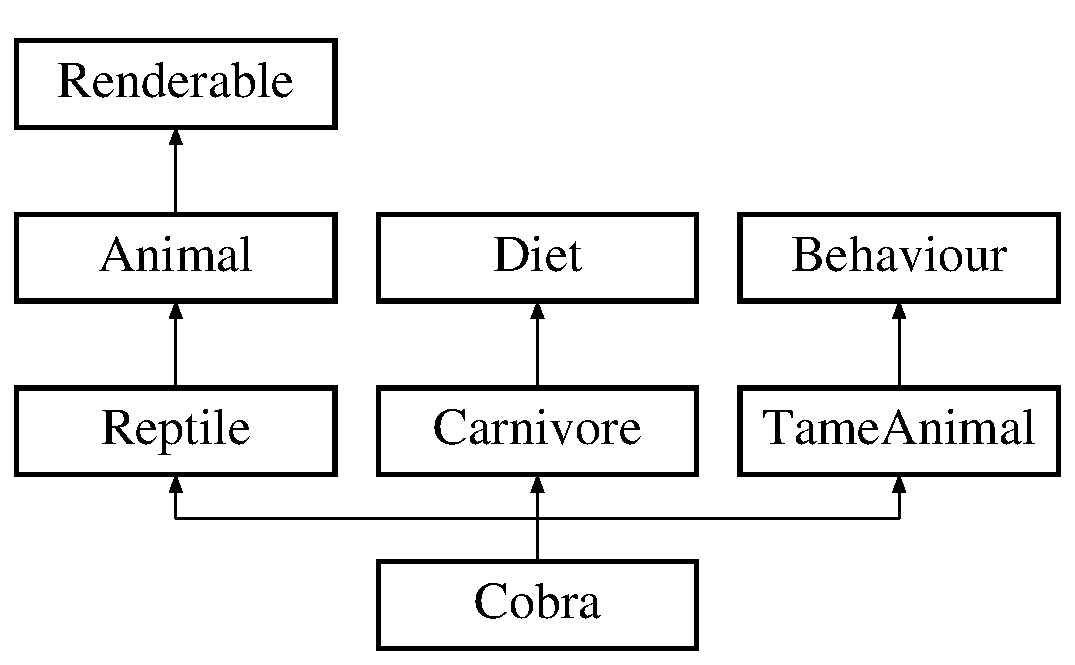
\includegraphics[height=4.000000cm]{classCobra}
\end{center}
\end{figure}
\subsection*{Public Member Functions}
\begin{DoxyCompactItemize}
\item 
\hypertarget{classCobra_afe3610c43386878eb1f80277933a20d0}{\hyperlink{classCobra_afe3610c43386878eb1f80277933a20d0}{Cobra} (int \+\_\+weight)}\label{classCobra_afe3610c43386878eb1f80277933a20d0}

\begin{DoxyCompactList}\small\item\em Constructor. Menciptakan ular kobra. \end{DoxyCompactList}\item 
string \hyperlink{classCobra_a4d93bcdfc9811547e3418818bec32585}{interact} () const 
\begin{DoxyCompactList}\small\item\em Melakukan interaksi dengan ular kobra. \end{DoxyCompactList}\end{DoxyCompactItemize}
\subsection*{Additional Inherited Members}


\subsection{Detailed Description}
Kelas \hyperlink{classCobra}{Cobra} yang merepesentasikan ular kobra. 

\subsection{Member Function Documentation}
\hypertarget{classCobra_a4d93bcdfc9811547e3418818bec32585}{\index{Cobra@{Cobra}!interact@{interact}}
\index{interact@{interact}!Cobra@{Cobra}}
\subsubsection[{interact}]{\setlength{\rightskip}{0pt plus 5cm}string Cobra\+::interact (
\begin{DoxyParamCaption}
{}
\end{DoxyParamCaption}
) const}}\label{classCobra_a4d93bcdfc9811547e3418818bec32585}


Melakukan interaksi dengan ular kobra. 

\begin{DoxyReturn}{Returns}
Experience yang dirasakan ketika berinteraksi dengan ular kobra. 
\end{DoxyReturn}


The documentation for this class was generated from the following files\+:\begin{DoxyCompactItemize}
\item 
src/\+Animal/\+Reptile/\+Cobra/Cobra.\+h\item 
src/\+Animal/\+Reptile/\+Cobra/Cobra.\+cpp\end{DoxyCompactItemize}

\hypertarget{classDiet}{\section{Diet Class Reference}
\label{classDiet}\index{Diet@{Diet}}
}


{\ttfamily \#include $<$Diet.\+h$>$}

Inheritance diagram for Diet\+:\begin{figure}[H]
\begin{center}
\leavevmode
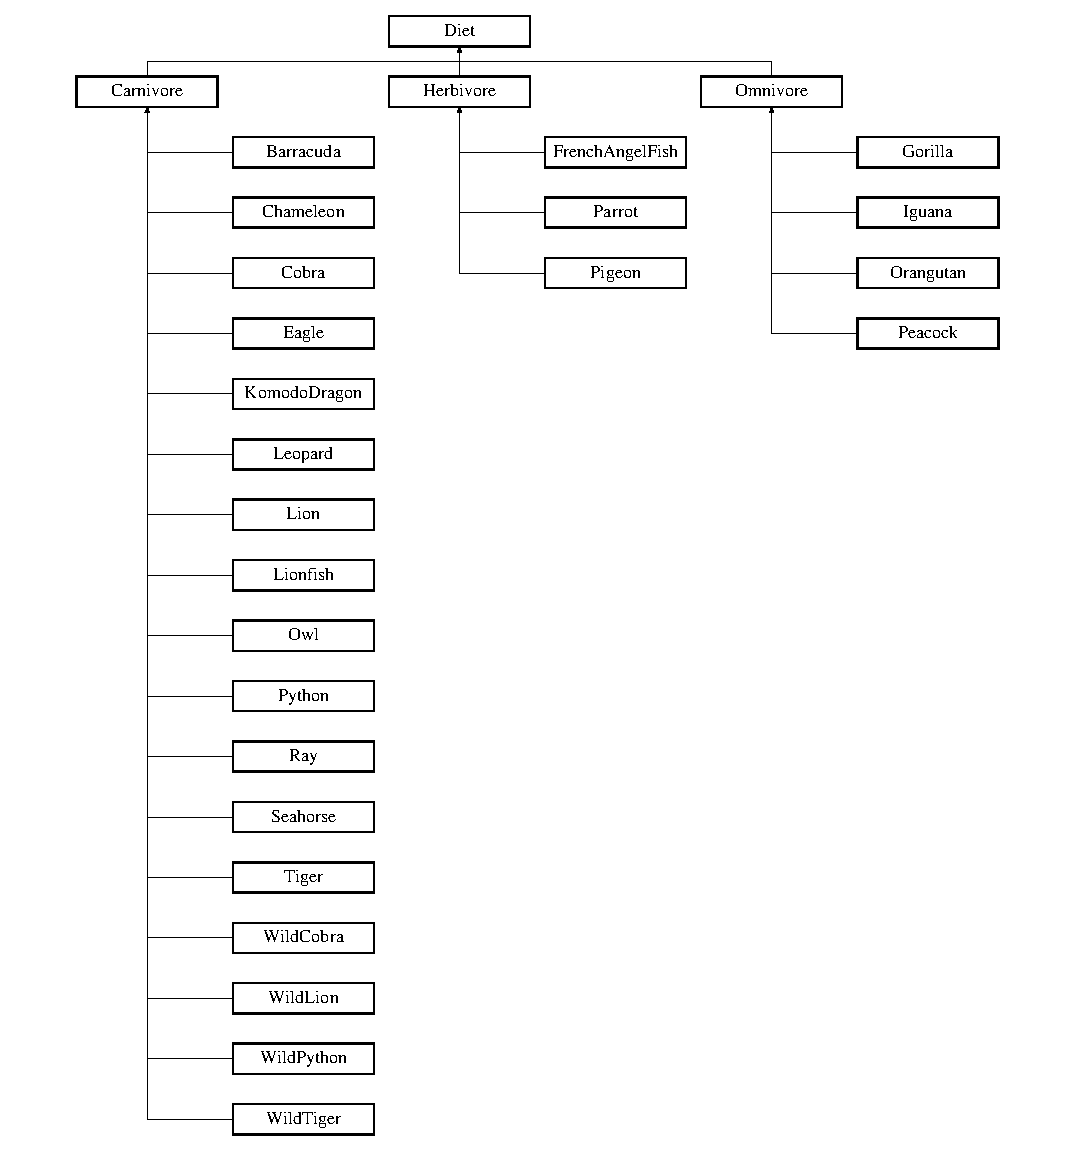
\includegraphics[height=12.000000cm]{classDiet}
\end{center}
\end{figure}
\subsection*{Public Member Functions}
\begin{DoxyCompactItemize}
\item 
\hypertarget{classDiet_a28b20982e580421a276d9059073e6282}{{\bfseries Diet} (int \+\_\+weight, double \+\_\+ratio)}\label{classDiet_a28b20982e580421a276d9059073e6282}

\item 
bool \hyperlink{classDiet_af8d66ff89a8ffed6da619bd9851590ea}{Is\+Carnivore} () const 
\begin{DoxyCompactList}\small\item\em Memeriksa apakah hewan karnivora atau tidak. \end{DoxyCompactList}\item 
bool \hyperlink{classDiet_ac26831907b06d6407433d560c64e122a}{Is\+Herbivore} () const 
\begin{DoxyCompactList}\small\item\em Memeriksa apakah hewan herbivora atau tidak. \end{DoxyCompactList}\item 
bool \hyperlink{classDiet_a48e33eb64393a4fddc72e01388aec451}{Is\+Omnivore} () const 
\begin{DoxyCompactList}\small\item\em Memeriksa apakah hewan omnivora atau tidak. \end{DoxyCompactList}\item 
int \hyperlink{classDiet_aa680acdabd171e868e3c828b86a06ae4}{calculate\+Total\+Food} () const 
\begin{DoxyCompactList}\small\item\em Menghitung banyaknya makanan yang dikonsumsi setiap hari relatif terhadap berat badannnya. \end{DoxyCompactList}\end{DoxyCompactItemize}
\subsection*{Protected Attributes}
\begin{DoxyCompactItemize}
\item 
\hypertarget{classDiet_a75c841392204d37f8f0963f171d103d5}{int {\bfseries weight}}\label{classDiet_a75c841392204d37f8f0963f171d103d5}

\item 
\hypertarget{classDiet_a1eacec1714a4af74478fe2d2ad14d705}{double {\bfseries ratio}}\label{classDiet_a1eacec1714a4af74478fe2d2ad14d705}

\item 
\hypertarget{classDiet_a5a961cb7f0e58e79815934be79c77014}{bool {\bfseries carnivore}}\label{classDiet_a5a961cb7f0e58e79815934be79c77014}

\item 
\hypertarget{classDiet_a96cf53475c6082be1b5a68ea656c1bb4}{bool {\bfseries herbivore}}\label{classDiet_a96cf53475c6082be1b5a68ea656c1bb4}

\end{DoxyCompactItemize}


\subsection{Detailed Description}
Kelas abstrak \hyperlink{classDiet}{Diet} yang merepesentasikan jenis makanan hewan. 

\subsection{Member Function Documentation}
\hypertarget{classDiet_aa680acdabd171e868e3c828b86a06ae4}{\index{Diet@{Diet}!calculate\+Total\+Food@{calculate\+Total\+Food}}
\index{calculate\+Total\+Food@{calculate\+Total\+Food}!Diet@{Diet}}
\subsubsection[{calculate\+Total\+Food}]{\setlength{\rightskip}{0pt plus 5cm}int Diet\+::calculate\+Total\+Food (
\begin{DoxyParamCaption}
{}
\end{DoxyParamCaption}
) const}}\label{classDiet_aa680acdabd171e868e3c828b86a06ae4}


Menghitung banyaknya makanan yang dikonsumsi setiap hari relatif terhadap berat badannnya. 

\begin{DoxyReturn}{Returns}
Banyaknya makanan yang dikonsumsi setiap hari. 
\end{DoxyReturn}
\hypertarget{classDiet_af8d66ff89a8ffed6da619bd9851590ea}{\index{Diet@{Diet}!Is\+Carnivore@{Is\+Carnivore}}
\index{Is\+Carnivore@{Is\+Carnivore}!Diet@{Diet}}
\subsubsection[{Is\+Carnivore}]{\setlength{\rightskip}{0pt plus 5cm}bool Diet\+::\+Is\+Carnivore (
\begin{DoxyParamCaption}
{}
\end{DoxyParamCaption}
) const}}\label{classDiet_af8d66ff89a8ffed6da619bd9851590ea}


Memeriksa apakah hewan karnivora atau tidak. 

\begin{DoxyReturn}{Returns}
True jika hewan adalah hewan karnivora dan False jika tidak. 
\end{DoxyReturn}
\hypertarget{classDiet_ac26831907b06d6407433d560c64e122a}{\index{Diet@{Diet}!Is\+Herbivore@{Is\+Herbivore}}
\index{Is\+Herbivore@{Is\+Herbivore}!Diet@{Diet}}
\subsubsection[{Is\+Herbivore}]{\setlength{\rightskip}{0pt plus 5cm}bool Diet\+::\+Is\+Herbivore (
\begin{DoxyParamCaption}
{}
\end{DoxyParamCaption}
) const}}\label{classDiet_ac26831907b06d6407433d560c64e122a}


Memeriksa apakah hewan herbivora atau tidak. 

\begin{DoxyReturn}{Returns}
True jika hewan adalah hewan herbivora dan False jika tidak. 
\end{DoxyReturn}
\hypertarget{classDiet_a48e33eb64393a4fddc72e01388aec451}{\index{Diet@{Diet}!Is\+Omnivore@{Is\+Omnivore}}
\index{Is\+Omnivore@{Is\+Omnivore}!Diet@{Diet}}
\subsubsection[{Is\+Omnivore}]{\setlength{\rightskip}{0pt plus 5cm}bool Diet\+::\+Is\+Omnivore (
\begin{DoxyParamCaption}
{}
\end{DoxyParamCaption}
) const}}\label{classDiet_a48e33eb64393a4fddc72e01388aec451}


Memeriksa apakah hewan omnivora atau tidak. 

\begin{DoxyReturn}{Returns}
True jika hewan adalah hewan omnivora dan False jika tidak. 
\end{DoxyReturn}


The documentation for this class was generated from the following files\+:\begin{DoxyCompactItemize}
\item 
src/\+Animal/\+Diet/Diet.\+h\item 
src/\+Animal/\+Diet/Diet.\+cpp\end{DoxyCompactItemize}

\hypertarget{classEagle}{\section{Eagle Class Reference}
\label{classEagle}\index{Eagle@{Eagle}}
}


{\ttfamily \#include $<$Eagle.\+h$>$}

Inheritance diagram for Eagle\+:\begin{figure}[H]
\begin{center}
\leavevmode
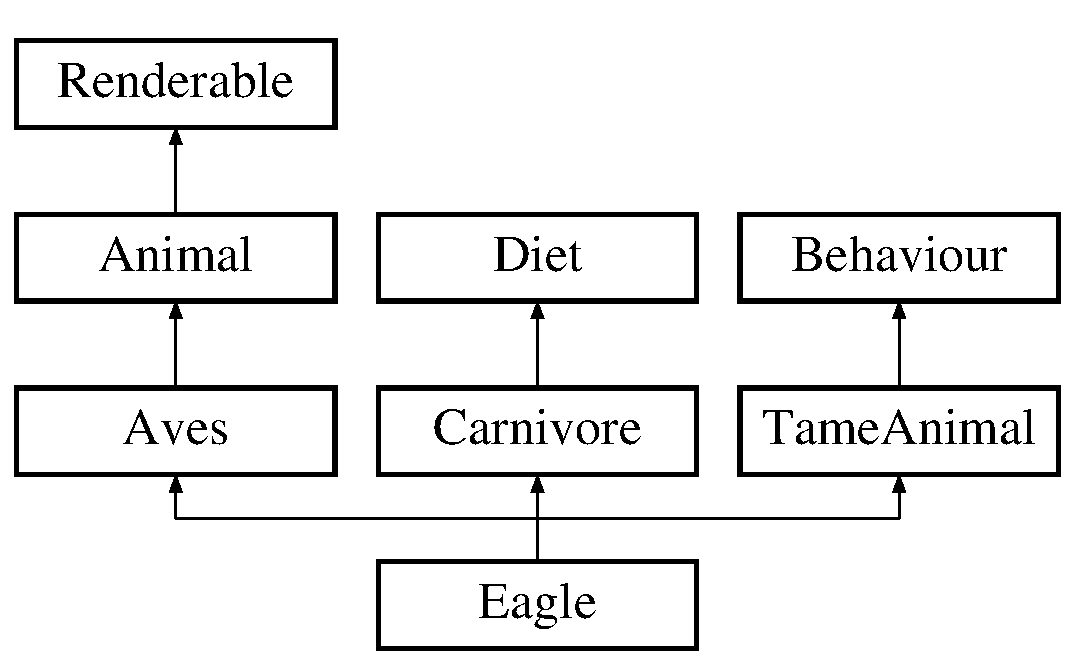
\includegraphics[height=4.000000cm]{classEagle}
\end{center}
\end{figure}
\subsection*{Public Member Functions}
\begin{DoxyCompactItemize}
\item 
\hypertarget{classEagle_ade1c532a412904896453a632974d1260}{\hyperlink{classEagle_ade1c532a412904896453a632974d1260}{Eagle} (int \+\_\+weight)}\label{classEagle_ade1c532a412904896453a632974d1260}

\begin{DoxyCompactList}\small\item\em Constructor. Menciptakan elang. \end{DoxyCompactList}\item 
string \hyperlink{classEagle_a9d5e9e67b1a4661bcab31bc13d951d57}{interact} () const 
\begin{DoxyCompactList}\small\item\em Melakukan interaksi dengan elang. \end{DoxyCompactList}\end{DoxyCompactItemize}
\subsection*{Additional Inherited Members}


\subsection{Detailed Description}
Kelas \hyperlink{classEagle}{Eagle} yang merepesentasikan elang. 

\subsection{Member Function Documentation}
\hypertarget{classEagle_a9d5e9e67b1a4661bcab31bc13d951d57}{\index{Eagle@{Eagle}!interact@{interact}}
\index{interact@{interact}!Eagle@{Eagle}}
\subsubsection[{interact}]{\setlength{\rightskip}{0pt plus 5cm}string Eagle\+::interact (
\begin{DoxyParamCaption}
{}
\end{DoxyParamCaption}
) const}}\label{classEagle_a9d5e9e67b1a4661bcab31bc13d951d57}


Melakukan interaksi dengan elang. 

\begin{DoxyReturn}{Returns}
Experience yang dirasakan ketika berinteraksi dengan elang. 
\end{DoxyReturn}


The documentation for this class was generated from the following files\+:\begin{DoxyCompactItemize}
\item 
src/\+Animal/\+Aves/\+Eagle/Eagle.\+h\item 
src/\+Animal/\+Aves/\+Eagle/Eagle.\+cpp\end{DoxyCompactItemize}

\hypertarget{classEntrance}{\section{Entrance Class Reference}
\label{classEntrance}\index{Entrance@{Entrance}}
}


{\ttfamily \#include $<$Entrance.\+h$>$}

Inheritance diagram for Entrance\+:\begin{figure}[H]
\begin{center}
\leavevmode
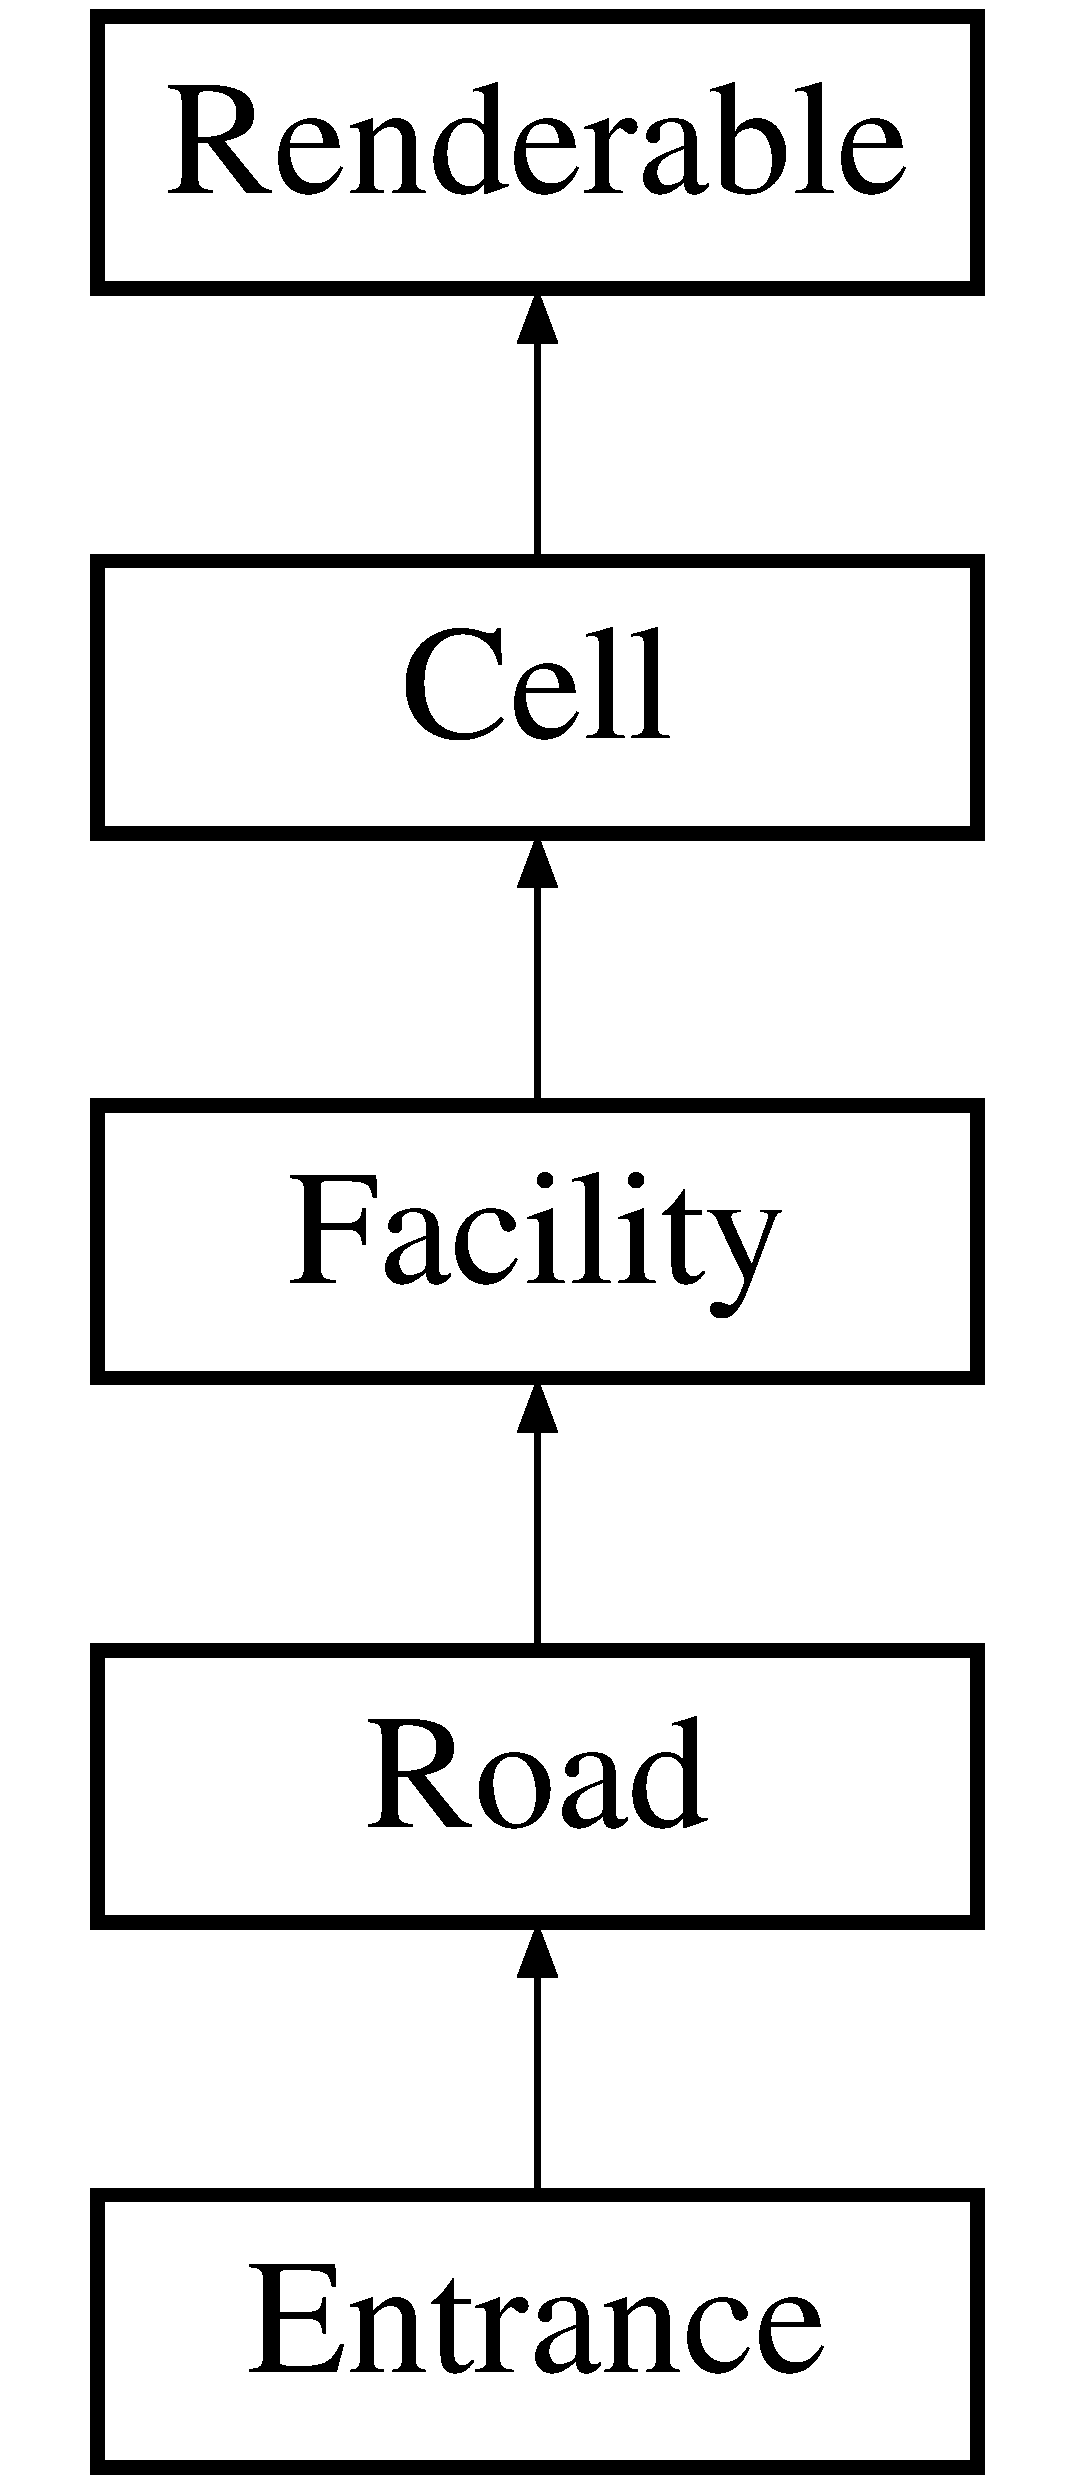
\includegraphics[height=5.000000cm]{classEntrance}
\end{center}
\end{figure}
\subsection*{Public Member Functions}
\begin{DoxyCompactItemize}
\item 
\hypertarget{classEntrance_a88cd27875093371afa47ac0f321716d7}{\hyperlink{classEntrance_a88cd27875093371afa47ac0f321716d7}{Entrance} ()}\label{classEntrance_a88cd27875093371afa47ac0f321716d7}

\begin{DoxyCompactList}\small\item\em Constructor. Menciptakan sebuah jalan masuk. \end{DoxyCompactList}\item 
\hypertarget{classEntrance_a05919fe3f4948ea3266b5dd4c5e119ac}{virtual \hyperlink{classEntrance_a05919fe3f4948ea3266b5dd4c5e119ac}{$\sim$\+Entrance} ()}\label{classEntrance_a05919fe3f4948ea3266b5dd4c5e119ac}

\begin{DoxyCompactList}\small\item\em Destructor. \end{DoxyCompactList}\end{DoxyCompactItemize}
\subsection*{Additional Inherited Members}


\subsection{Detailed Description}
Kelas \hyperlink{classEntrance}{Entrance} yang merepesentasikan jalan masuk. 

The documentation for this class was generated from the following files\+:\begin{DoxyCompactItemize}
\item 
src/\+Cell/\+Facility/\+Road/\+Entrance/Entrance.\+h\item 
src/\+Cell/\+Facility/\+Road/\+Entrance/Entrance.\+cpp\end{DoxyCompactItemize}

\hypertarget{classExit}{\section{Exit Class Reference}
\label{classExit}\index{Exit@{Exit}}
}


{\ttfamily \#include $<$Exit.\+h$>$}

Inheritance diagram for Exit\+:\begin{figure}[H]
\begin{center}
\leavevmode
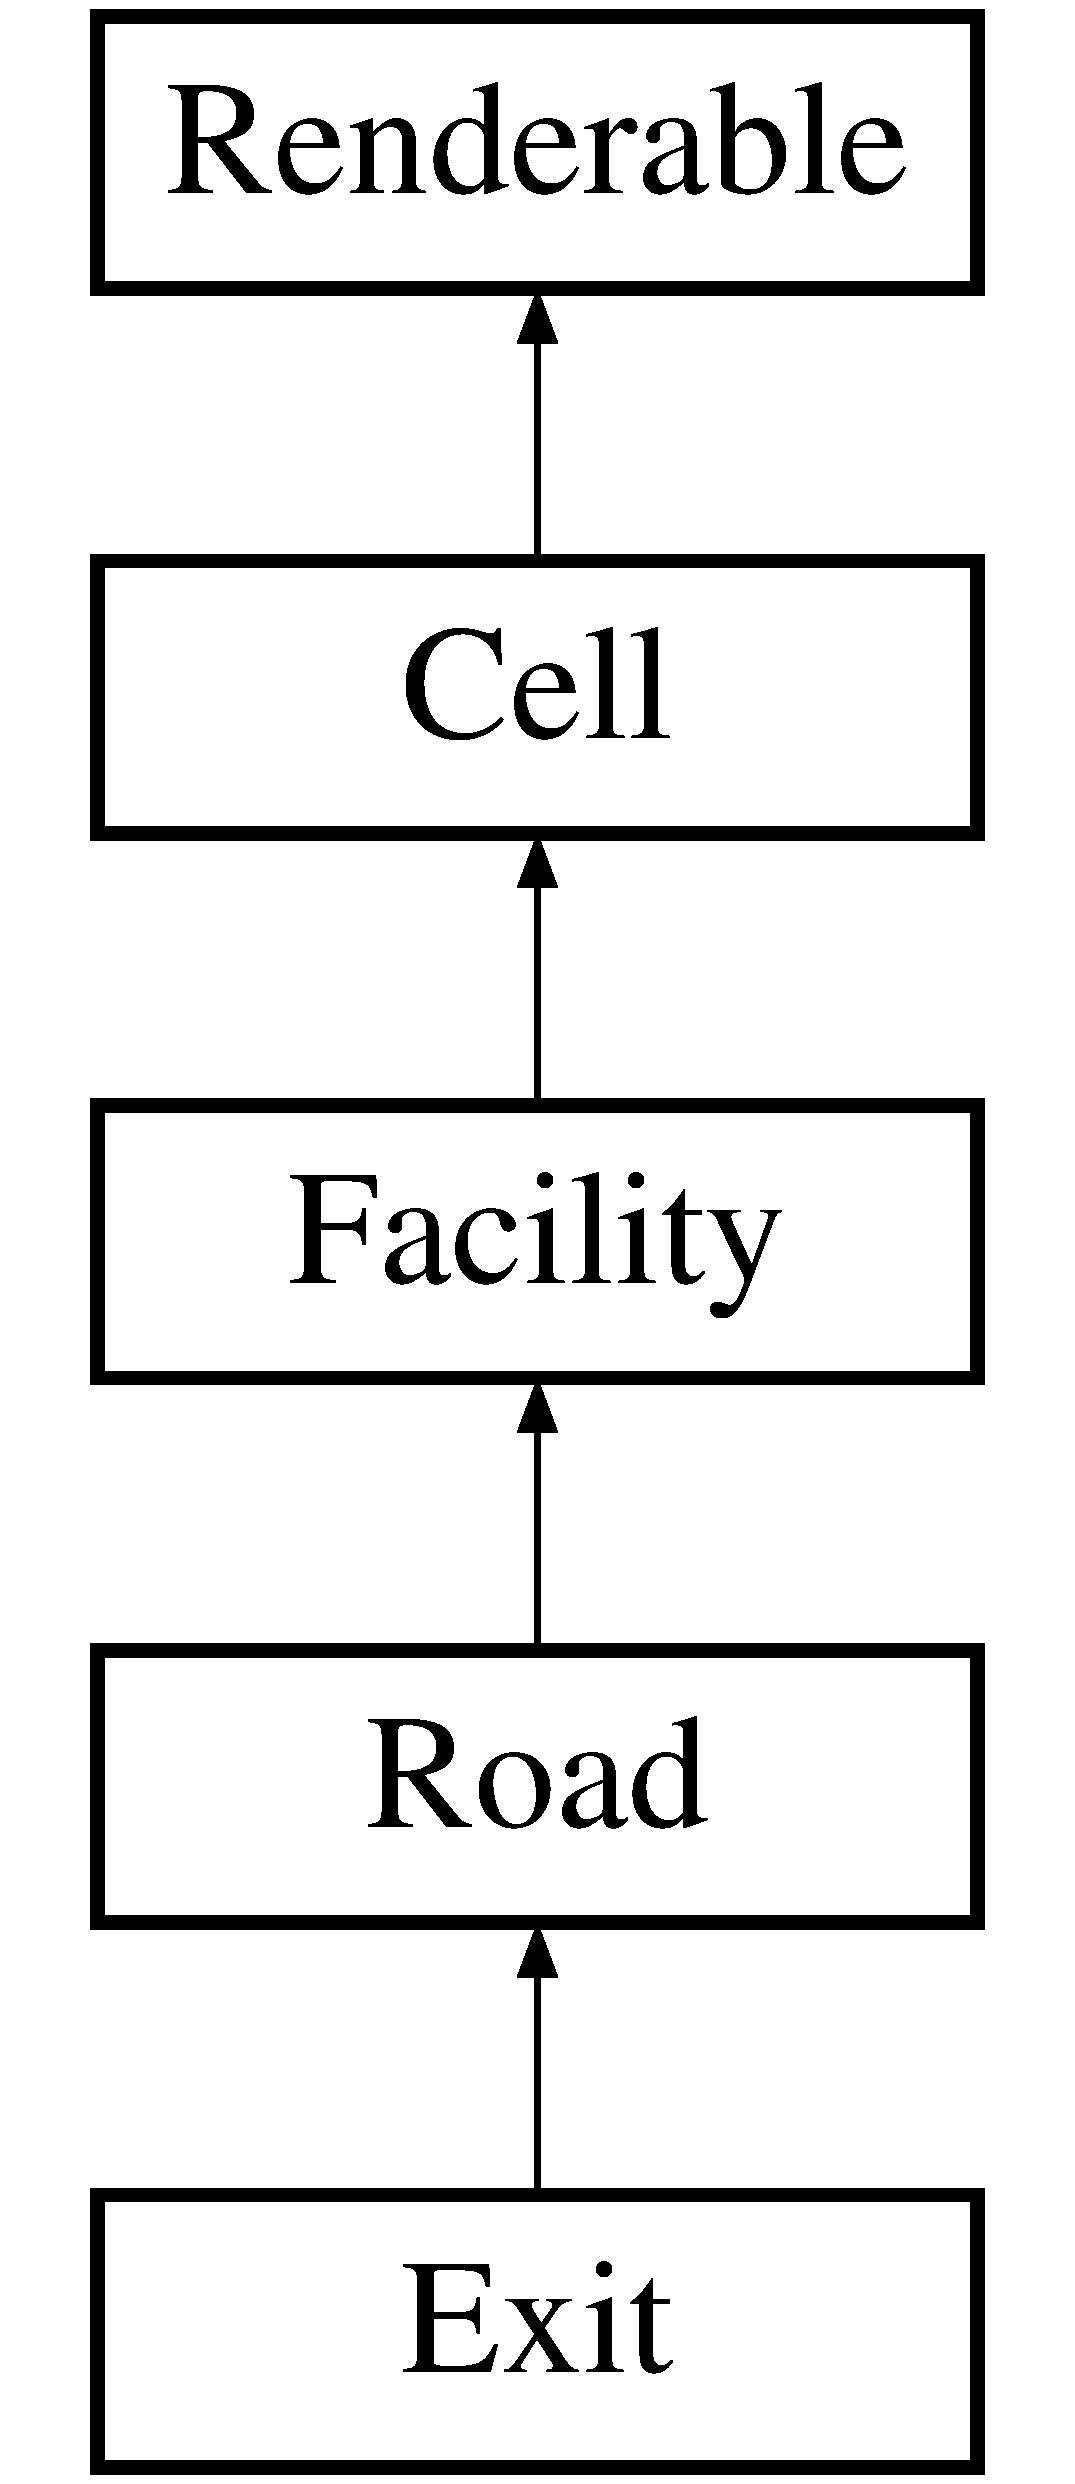
\includegraphics[height=5.000000cm]{classExit}
\end{center}
\end{figure}
\subsection*{Public Member Functions}
\begin{DoxyCompactItemize}
\item 
\hypertarget{classExit_a9b2f58ee65af58d03d7004d9fc2ab264}{\hyperlink{classExit_a9b2f58ee65af58d03d7004d9fc2ab264}{Exit} ()}\label{classExit_a9b2f58ee65af58d03d7004d9fc2ab264}

\begin{DoxyCompactList}\small\item\em Constructor. Menciptakan sebuah jalan keluar. \end{DoxyCompactList}\item 
\hypertarget{classExit_adf66e70ca988ae2fe7e74ef256d8612a}{virtual \hyperlink{classExit_adf66e70ca988ae2fe7e74ef256d8612a}{$\sim$\+Exit} ()}\label{classExit_adf66e70ca988ae2fe7e74ef256d8612a}

\begin{DoxyCompactList}\small\item\em Destructor. \end{DoxyCompactList}\end{DoxyCompactItemize}
\subsection*{Additional Inherited Members}


\subsection{Detailed Description}
Kelas \hyperlink{classExit}{Exit} yang merepesentasikan jalan keluar. 

The documentation for this class was generated from the following files\+:\begin{DoxyCompactItemize}
\item 
src/\+Cell/\+Facility/\+Road/\+Exit/Exit.\+h\item 
src/\+Cell/\+Facility/\+Road/\+Exit/Exit.\+cpp\end{DoxyCompactItemize}

\hypertarget{classFacility}{\section{Facility Class Reference}
\label{classFacility}\index{Facility@{Facility}}
}


{\ttfamily \#include $<$Facility.\+h$>$}

Inheritance diagram for Facility\+:\begin{figure}[H]
\begin{center}
\leavevmode
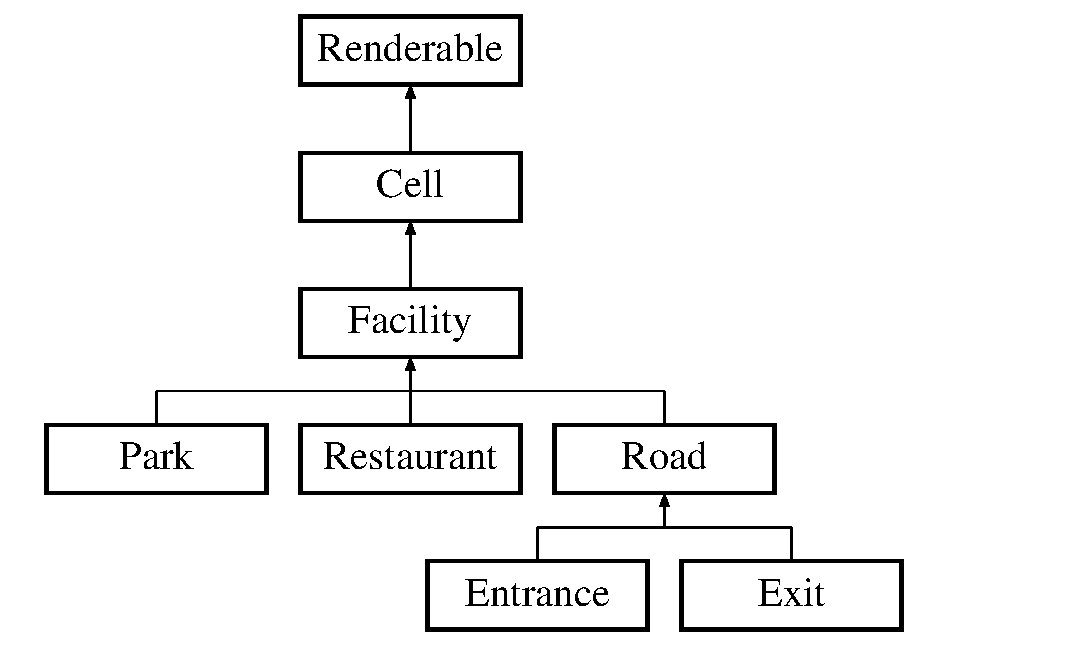
\includegraphics[height=5.000000cm]{classFacility}
\end{center}
\end{figure}
\subsection*{Public Member Functions}
\begin{DoxyCompactItemize}
\item 
\hyperlink{classFacility_a9b41510329095aeb06232f06af2d4152}{Facility} (bool \+\_\+accessible, char \+\_\+facility\+Type)
\begin{DoxyCompactList}\small\item\em Constructor. Menciptakan sebuah fasilitas dengan status aksesibilitas dan jenis tertentu. \end{DoxyCompactList}\item 
\hypertarget{classFacility_a0d756a7273f5cb2fc57575459ba45670}{virtual \hyperlink{classFacility_a0d756a7273f5cb2fc57575459ba45670}{$\sim$\+Facility} ()}\label{classFacility_a0d756a7273f5cb2fc57575459ba45670}

\begin{DoxyCompactList}\small\item\em Destructor. \end{DoxyCompactList}\end{DoxyCompactItemize}
\subsection*{Protected Attributes}
\begin{DoxyCompactItemize}
\item 
\hypertarget{classFacility_a55542247d165c099f791dc41c1eda23e}{char {\bfseries facility\+Type}}\label{classFacility_a55542247d165c099f791dc41c1eda23e}

\end{DoxyCompactItemize}


\subsection{Detailed Description}
Kelas abstrak \hyperlink{classFacility}{Facility} yang merepesentasikan petak tanah berukuran 1m x 1m yang merupakan fasilitas. 

\subsection{Constructor \& Destructor Documentation}
\hypertarget{classFacility_a9b41510329095aeb06232f06af2d4152}{\index{Facility@{Facility}!Facility@{Facility}}
\index{Facility@{Facility}!Facility@{Facility}}
\subsubsection[{Facility}]{\setlength{\rightskip}{0pt plus 5cm}Facility\+::\+Facility (
\begin{DoxyParamCaption}
\item[{bool}]{\+\_\+accessible, }
\item[{char}]{\+\_\+facility\+Type}
\end{DoxyParamCaption}
)}}\label{classFacility_a9b41510329095aeb06232f06af2d4152}


Constructor. Menciptakan sebuah fasilitas dengan status aksesibilitas dan jenis tertentu. 


\begin{DoxyParams}{Parameters}
{\em \+\_\+accessible} & Status aksesibiltas fasilitas. \\
\hline
{\em \+\_\+facility\+Type} & Jenis dari fasilitas. \\
\hline
\end{DoxyParams}


The documentation for this class was generated from the following files\+:\begin{DoxyCompactItemize}
\item 
src/\+Cell/\+Facility/Facility.\+h\item 
src/\+Cell/\+Facility/Facility.\+cpp\end{DoxyCompactItemize}

\hypertarget{classFrenchAngelFish}{\section{French\+Angel\+Fish Class Reference}
\label{classFrenchAngelFish}\index{French\+Angel\+Fish@{French\+Angel\+Fish}}
}


{\ttfamily \#include $<$French\+Angel\+Fish.\+h$>$}

Inheritance diagram for French\+Angel\+Fish\+:\begin{figure}[H]
\begin{center}
\leavevmode
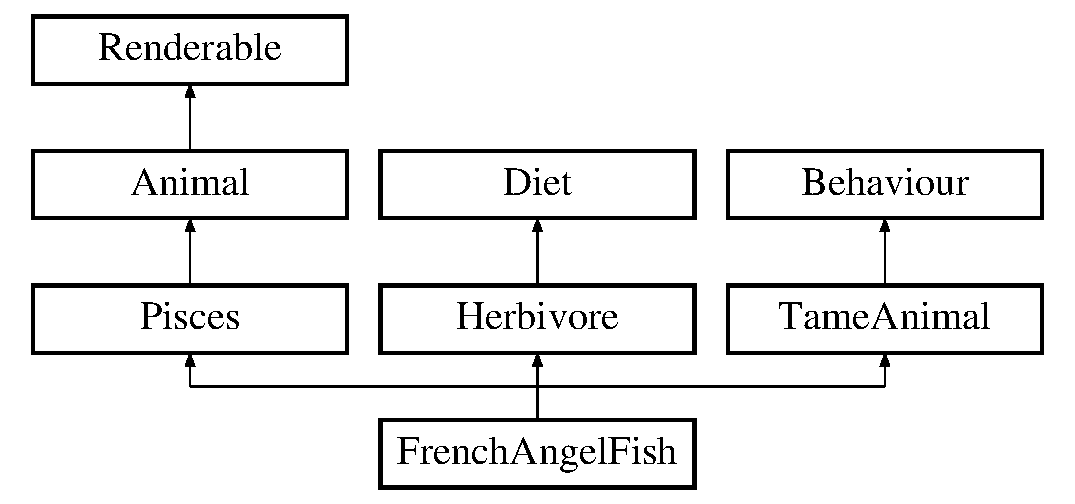
\includegraphics[height=4.000000cm]{classFrenchAngelFish}
\end{center}
\end{figure}
\subsection*{Public Member Functions}
\begin{DoxyCompactItemize}
\item 
\hypertarget{classFrenchAngelFish_ae87d13dbe9c9ccd8abdfd1b877add9d2}{\hyperlink{classFrenchAngelFish_ae87d13dbe9c9ccd8abdfd1b877add9d2}{French\+Angel\+Fish} (int \+\_\+weight)}\label{classFrenchAngelFish_ae87d13dbe9c9ccd8abdfd1b877add9d2}

\begin{DoxyCompactList}\small\item\em Constructor. Menciptakan french angelfish. \end{DoxyCompactList}\item 
string \hyperlink{classFrenchAngelFish_a57bb0a609dcb55fac08f7e32f01319c8}{interact} () const 
\begin{DoxyCompactList}\small\item\em Melakukan interaksi dengan french angelfish. \end{DoxyCompactList}\end{DoxyCompactItemize}
\subsection*{Additional Inherited Members}


\subsection{Detailed Description}
Kelas \hyperlink{classFrenchAngelFish}{French\+Angel\+Fish} yang merepesentasikan french angelfish. 

\subsection{Member Function Documentation}
\hypertarget{classFrenchAngelFish_a57bb0a609dcb55fac08f7e32f01319c8}{\index{French\+Angel\+Fish@{French\+Angel\+Fish}!interact@{interact}}
\index{interact@{interact}!French\+Angel\+Fish@{French\+Angel\+Fish}}
\subsubsection[{interact}]{\setlength{\rightskip}{0pt plus 5cm}string French\+Angel\+Fish\+::interact (
\begin{DoxyParamCaption}
{}
\end{DoxyParamCaption}
) const}}\label{classFrenchAngelFish_a57bb0a609dcb55fac08f7e32f01319c8}


Melakukan interaksi dengan french angelfish. 

\begin{DoxyReturn}{Returns}
Experience yang dirasakan ketika berinteraksi dengan french angelfish. 
\end{DoxyReturn}


The documentation for this class was generated from the following files\+:\begin{DoxyCompactItemize}
\item 
src/\+Animal/\+Pisces/\+French\+Angel\+Fish/French\+Angel\+Fish.\+h\item 
src/\+Animal/\+Pisces/\+French\+Angel\+Fish/French\+Angel\+Fish.\+cpp\end{DoxyCompactItemize}

\hypertarget{classGorilla}{\section{Gorilla Class Reference}
\label{classGorilla}\index{Gorilla@{Gorilla}}
}


{\ttfamily \#include $<$Gorilla.\+h$>$}

Inheritance diagram for Gorilla\+:\begin{figure}[H]
\begin{center}
\leavevmode
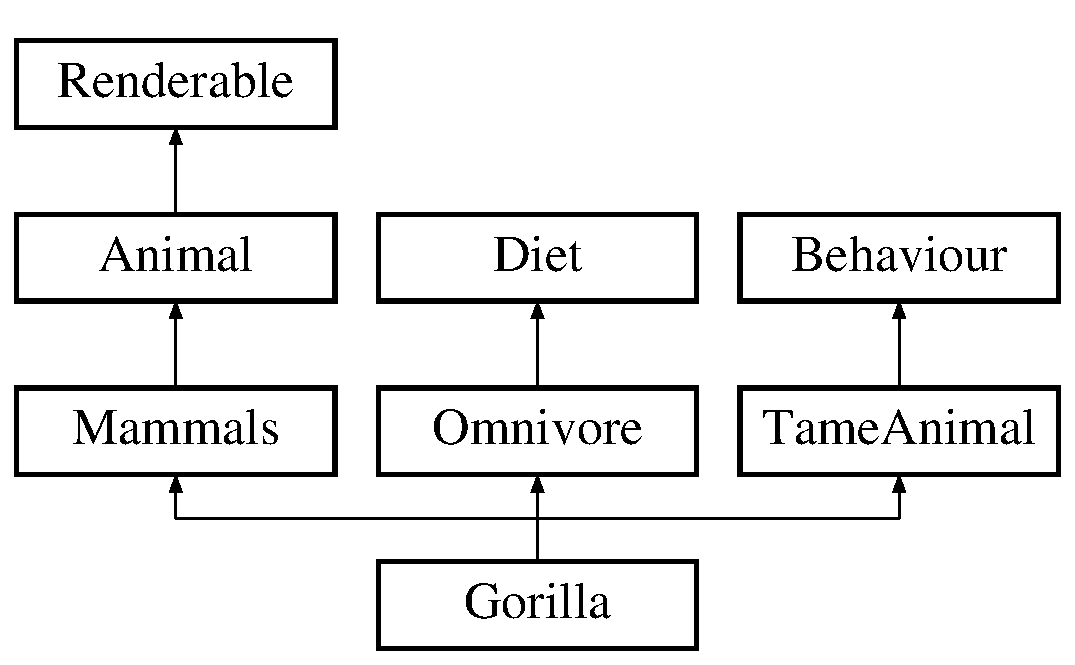
\includegraphics[height=4.000000cm]{classGorilla}
\end{center}
\end{figure}
\subsection*{Public Member Functions}
\begin{DoxyCompactItemize}
\item 
\hypertarget{classGorilla_a242f07524eed46be55f48e9779ad9ec5}{\hyperlink{classGorilla_a242f07524eed46be55f48e9779ad9ec5}{Gorilla} (int \+\_\+weight)}\label{classGorilla_a242f07524eed46be55f48e9779ad9ec5}

\begin{DoxyCompactList}\small\item\em Constructor. Menciptakan gorilla. \end{DoxyCompactList}\item 
string \hyperlink{classGorilla_acb6db934144c2616f5cac01045eb0535}{interact} () const 
\begin{DoxyCompactList}\small\item\em Melakukan interaksi dengan gorilla. \end{DoxyCompactList}\end{DoxyCompactItemize}
\subsection*{Additional Inherited Members}


\subsection{Detailed Description}
Kelas \hyperlink{classGorilla}{Gorilla} yang merepesentasikan gorilla. 

\subsection{Member Function Documentation}
\hypertarget{classGorilla_acb6db934144c2616f5cac01045eb0535}{\index{Gorilla@{Gorilla}!interact@{interact}}
\index{interact@{interact}!Gorilla@{Gorilla}}
\subsubsection[{interact}]{\setlength{\rightskip}{0pt plus 5cm}string Gorilla\+::interact (
\begin{DoxyParamCaption}
{}
\end{DoxyParamCaption}
) const}}\label{classGorilla_acb6db934144c2616f5cac01045eb0535}


Melakukan interaksi dengan gorilla. 

\begin{DoxyReturn}{Returns}
Experience yang dirasakan ketika berinteraksi dengan gorilla. 
\end{DoxyReturn}


The documentation for this class was generated from the following files\+:\begin{DoxyCompactItemize}
\item 
src/\+Animal/\+Mammals/\+Gorilla/Gorilla.\+h\item 
src/\+Animal/\+Mammals/\+Gorilla/Gorilla.\+cpp\end{DoxyCompactItemize}

\hypertarget{classHabitat}{\section{Habitat Class Reference}
\label{classHabitat}\index{Habitat@{Habitat}}
}


{\ttfamily \#include $<$Habitat.\+h$>$}

Inheritance diagram for Habitat\+:\begin{figure}[H]
\begin{center}
\leavevmode
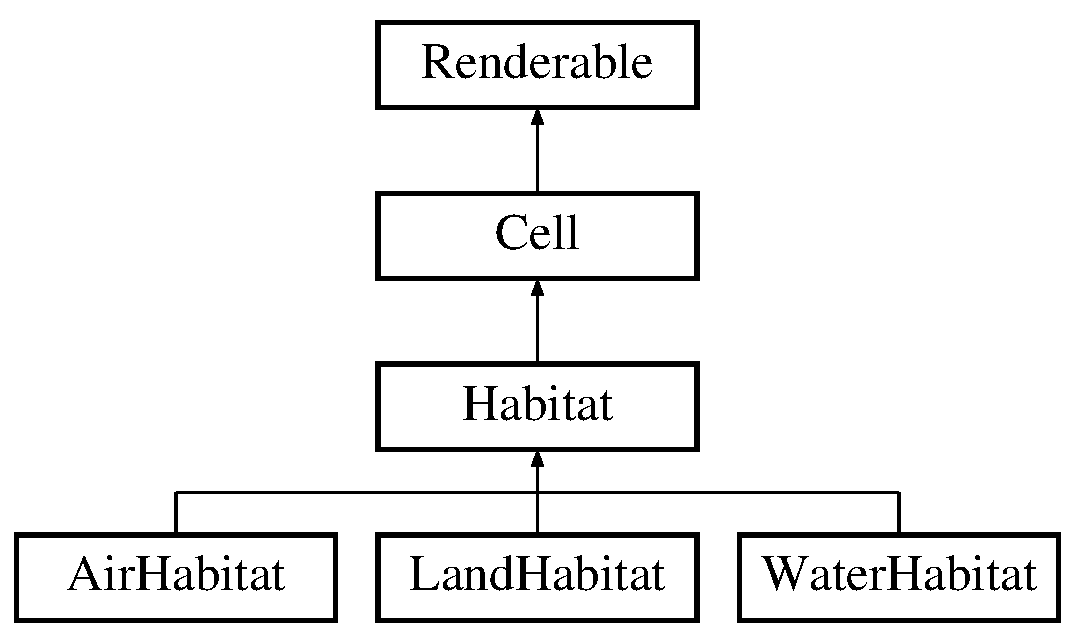
\includegraphics[height=4.000000cm]{classHabitat}
\end{center}
\end{figure}
\subsection*{Public Member Functions}
\begin{DoxyCompactItemize}
\item 
\hyperlink{classHabitat_ac227e66c09b35766737201b623fb7066}{Habitat} (char \+\_\+habitat\+Type)
\begin{DoxyCompactList}\small\item\em Constructor. Menciptakan sebuah \hyperlink{classHabitat}{Habitat} dengan jenis tertentu. \hyperlink{classHabitat}{Habitat} tidak dapat diakses. \end{DoxyCompactList}\item 
\hypertarget{classHabitat_afd413e46df54891b04262872f04b314f}{virtual \hyperlink{classHabitat_afd413e46df54891b04262872f04b314f}{$\sim$\+Habitat} ()}\label{classHabitat_afd413e46df54891b04262872f04b314f}

\begin{DoxyCompactList}\small\item\em Destructor. \end{DoxyCompactList}\end{DoxyCompactItemize}
\subsection*{Protected Attributes}
\begin{DoxyCompactItemize}
\item 
\hypertarget{classHabitat_a317eb1973b2d0702a78a1fdd3041c959}{char {\bfseries habitat\+Type}}\label{classHabitat_a317eb1973b2d0702a78a1fdd3041c959}

\end{DoxyCompactItemize}


\subsection{Detailed Description}
Kelas abstrak \hyperlink{classHabitat}{Habitat} yang merepesentasikan petak tanah berukuran 1m x 1m yang merupakan habitat. 

\subsection{Constructor \& Destructor Documentation}
\hypertarget{classHabitat_ac227e66c09b35766737201b623fb7066}{\index{Habitat@{Habitat}!Habitat@{Habitat}}
\index{Habitat@{Habitat}!Habitat@{Habitat}}
\subsubsection[{Habitat}]{\setlength{\rightskip}{0pt plus 5cm}Habitat\+::\+Habitat (
\begin{DoxyParamCaption}
\item[{char}]{\+\_\+habitat\+Type}
\end{DoxyParamCaption}
)}}\label{classHabitat_ac227e66c09b35766737201b623fb7066}


Constructor. Menciptakan sebuah \hyperlink{classHabitat}{Habitat} dengan jenis tertentu. \hyperlink{classHabitat}{Habitat} tidak dapat diakses. 


\begin{DoxyParams}{Parameters}
{\em \+\_\+habitat\+Type} & Jenis dari habitat. \\
\hline
\end{DoxyParams}


The documentation for this class was generated from the following files\+:\begin{DoxyCompactItemize}
\item 
src/\+Cell/\+Habitat/Habitat.\+h\item 
src/\+Cell/\+Habitat/Habitat.\+cpp\end{DoxyCompactItemize}

\hypertarget{classHerbivore}{\section{Herbivore Class Reference}
\label{classHerbivore}\index{Herbivore@{Herbivore}}
}
Inheritance diagram for Herbivore\+:\begin{figure}[H]
\begin{center}
\leavevmode
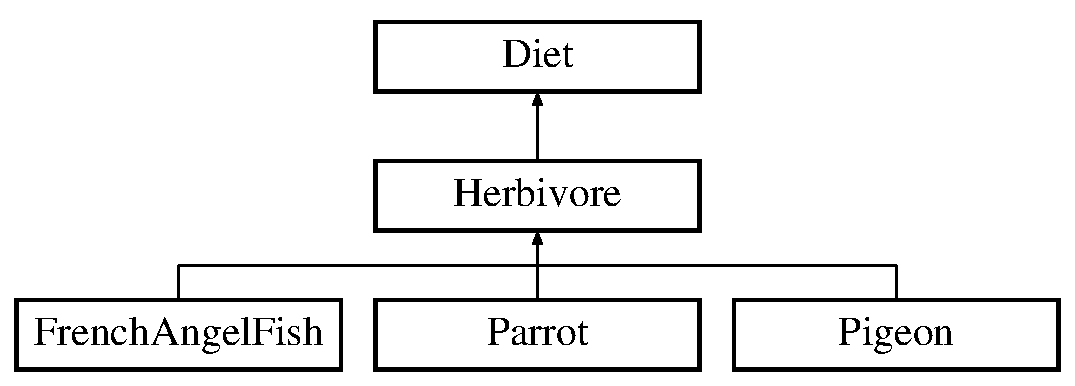
\includegraphics[height=3.000000cm]{classHerbivore}
\end{center}
\end{figure}
\subsection*{Public Member Functions}
\begin{DoxyCompactItemize}
\item 
\hyperlink{classHerbivore_a16d8cf2bbd4a830b80fa08678fab2ff6}{Herbivore} (int \+\_\+weight, double \+\_\+ratio)
\begin{DoxyCompactList}\small\item\em Constructor. Menciptakan hewan herbivora dengan berat tertentu. \end{DoxyCompactList}\end{DoxyCompactItemize}
\subsection*{Additional Inherited Members}


\subsection{Constructor \& Destructor Documentation}
\hypertarget{classHerbivore_a16d8cf2bbd4a830b80fa08678fab2ff6}{\index{Herbivore@{Herbivore}!Herbivore@{Herbivore}}
\index{Herbivore@{Herbivore}!Herbivore@{Herbivore}}
\subsubsection[{Herbivore}]{\setlength{\rightskip}{0pt plus 5cm}Herbivore\+::\+Herbivore (
\begin{DoxyParamCaption}
\item[{int}]{\+\_\+weight, }
\item[{double}]{\+\_\+ratio}
\end{DoxyParamCaption}
)}}\label{classHerbivore_a16d8cf2bbd4a830b80fa08678fab2ff6}


Constructor. Menciptakan hewan herbivora dengan berat tertentu. 


\begin{DoxyParams}{Parameters}
{\em \+\_\+weight} & Berat dari hewan. \\
\hline
\end{DoxyParams}


The documentation for this class was generated from the following files\+:\begin{DoxyCompactItemize}
\item 
src/\+Animal/\+Diet/\+Herbivore/Herbivore.\+h\item 
src/\+Animal/\+Diet/\+Herbivore/Herbivore.\+cpp\end{DoxyCompactItemize}

\hypertarget{classIguana}{\section{Iguana Class Reference}
\label{classIguana}\index{Iguana@{Iguana}}
}


{\ttfamily \#include $<$Iguana.\+h$>$}

Inheritance diagram for Iguana\+:\begin{figure}[H]
\begin{center}
\leavevmode
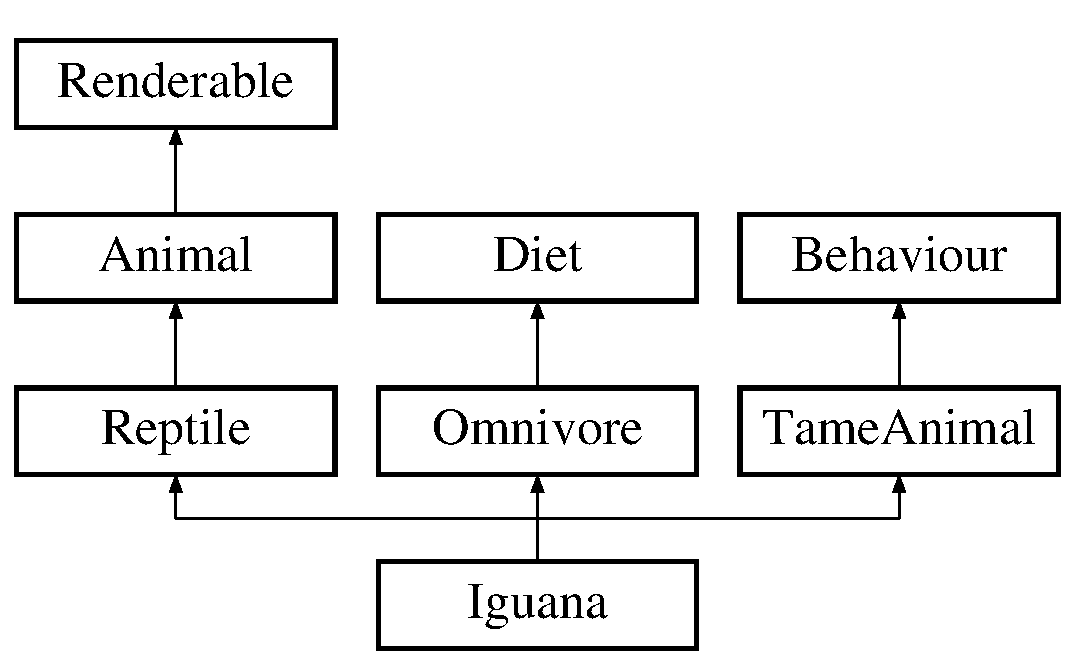
\includegraphics[height=4.000000cm]{classIguana}
\end{center}
\end{figure}
\subsection*{Public Member Functions}
\begin{DoxyCompactItemize}
\item 
\hypertarget{classIguana_a009dd4f985d9b6c32ce1283ba4f12e7c}{\hyperlink{classIguana_a009dd4f985d9b6c32ce1283ba4f12e7c}{Iguana} (int \+\_\+weight)}\label{classIguana_a009dd4f985d9b6c32ce1283ba4f12e7c}

\begin{DoxyCompactList}\small\item\em Constructor. Menciptakan iguana. \end{DoxyCompactList}\item 
string \hyperlink{classIguana_a2787eee87f7b90e905de0bf75012cb18}{interact} () const 
\begin{DoxyCompactList}\small\item\em Melakukan interaksi dengan iguana. \end{DoxyCompactList}\end{DoxyCompactItemize}
\subsection*{Additional Inherited Members}


\subsection{Detailed Description}
Kelas \hyperlink{classIguana}{Iguana} yang merepesentasikan iguana. 

\subsection{Member Function Documentation}
\hypertarget{classIguana_a2787eee87f7b90e905de0bf75012cb18}{\index{Iguana@{Iguana}!interact@{interact}}
\index{interact@{interact}!Iguana@{Iguana}}
\subsubsection[{interact}]{\setlength{\rightskip}{0pt plus 5cm}string Iguana\+::interact (
\begin{DoxyParamCaption}
{}
\end{DoxyParamCaption}
) const}}\label{classIguana_a2787eee87f7b90e905de0bf75012cb18}


Melakukan interaksi dengan iguana. 

\begin{DoxyReturn}{Returns}
Experience yang dirasakan ketika berinteraksi dengan iguana. 
\end{DoxyReturn}


The documentation for this class was generated from the following files\+:\begin{DoxyCompactItemize}
\item 
src/\+Animal/\+Reptile/\+Iguana/Iguana.\+h\item 
src/\+Animal/\+Reptile/\+Iguana/Iguana.\+cpp\end{DoxyCompactItemize}

\hypertarget{classTameAnimal_1_1Kelas}{\section{Tame\+Animal\+:\+:Kelas Class Reference}
\label{classTameAnimal_1_1Kelas}\index{Tame\+Animal\+::\+Kelas@{Tame\+Animal\+::\+Kelas}}
}


\subsection{Detailed Description}
merepresentasikan hewan jinak. 

The documentation for this class was generated from the following file\+:\begin{DoxyCompactItemize}
\item 
src/\+Animal/\+Behaviour/\+Tame\+Animal/Tame\+Animal.\+h\end{DoxyCompactItemize}

\hypertarget{classBehaviour_1_1Kelas}{\section{Behaviour\+:\+:Kelas Class Reference}
\label{classBehaviour_1_1Kelas}\index{Behaviour\+::\+Kelas@{Behaviour\+::\+Kelas}}
}


\subsection{Detailed Description}
merepresentasikan hewan dengan kelakukan tertentu (buas atau jinak). 

The documentation for this class was generated from the following file\+:\begin{DoxyCompactItemize}
\item 
src/\+Animal/\+Behaviour/Behaviour.\+h\end{DoxyCompactItemize}

\hypertarget{classWildAnimal_1_1Kelas}{\section{Wild\+Animal\+:\+:Kelas Class Reference}
\label{classWildAnimal_1_1Kelas}\index{Wild\+Animal\+::\+Kelas@{Wild\+Animal\+::\+Kelas}}
}


\subsection{Detailed Description}
merepresentasikan hewan buas. 

The documentation for this class was generated from the following file\+:\begin{DoxyCompactItemize}
\item 
src/\+Animal/\+Behaviour/\+Wild\+Animal/Wild\+Animal.\+h\end{DoxyCompactItemize}

\hypertarget{classKomodoDragon}{\section{Komodo\+Dragon Class Reference}
\label{classKomodoDragon}\index{Komodo\+Dragon@{Komodo\+Dragon}}
}


{\ttfamily \#include $<$Komodo\+Dragon.\+h$>$}

Inheritance diagram for Komodo\+Dragon\+:\begin{figure}[H]
\begin{center}
\leavevmode
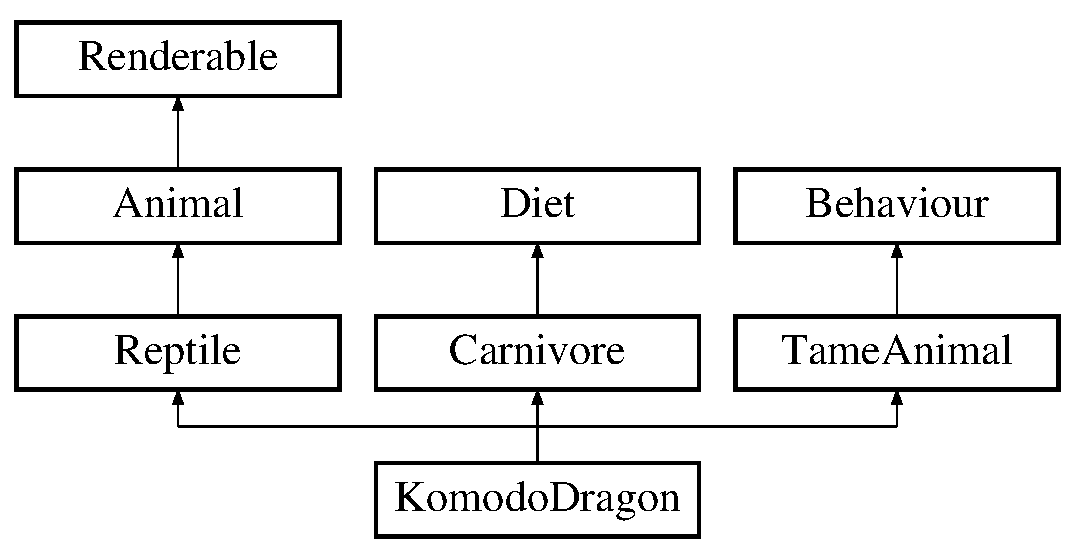
\includegraphics[height=4.000000cm]{classKomodoDragon}
\end{center}
\end{figure}
\subsection*{Public Member Functions}
\begin{DoxyCompactItemize}
\item 
\hypertarget{classKomodoDragon_a4426d1f077191ccf5e1ace6aebf17489}{\hyperlink{classKomodoDragon_a4426d1f077191ccf5e1ace6aebf17489}{Komodo\+Dragon} (int \+\_\+weight)}\label{classKomodoDragon_a4426d1f077191ccf5e1ace6aebf17489}

\begin{DoxyCompactList}\small\item\em Constructor. Menciptakan komodo. \end{DoxyCompactList}\item 
string \hyperlink{classKomodoDragon_ae6a9ac6072e527cba59bd9f36bd592a7}{interact} () const 
\begin{DoxyCompactList}\small\item\em Melakukan interaksi dengan komodo. \end{DoxyCompactList}\end{DoxyCompactItemize}
\subsection*{Additional Inherited Members}


\subsection{Detailed Description}
Kelas \hyperlink{classKomodoDragon}{Komodo\+Dragon} yang merepesentasikan komodo. 

\subsection{Member Function Documentation}
\hypertarget{classKomodoDragon_ae6a9ac6072e527cba59bd9f36bd592a7}{\index{Komodo\+Dragon@{Komodo\+Dragon}!interact@{interact}}
\index{interact@{interact}!Komodo\+Dragon@{Komodo\+Dragon}}
\subsubsection[{interact}]{\setlength{\rightskip}{0pt plus 5cm}string Komodo\+Dragon\+::interact (
\begin{DoxyParamCaption}
{}
\end{DoxyParamCaption}
) const}}\label{classKomodoDragon_ae6a9ac6072e527cba59bd9f36bd592a7}


Melakukan interaksi dengan komodo. 

\begin{DoxyReturn}{Returns}
Experience yang dirasakan ketika berinteraksi dengan komodo. 
\end{DoxyReturn}


The documentation for this class was generated from the following files\+:\begin{DoxyCompactItemize}
\item 
src/\+Animal/\+Reptile/\+Komodo\+Dragon/Komodo\+Dragon.\+h\item 
src/\+Animal/\+Reptile/\+Komodo\+Dragon/Komodo\+Dragon.\+cpp\end{DoxyCompactItemize}

\hypertarget{classLandHabitat}{\section{Land\+Habitat Class Reference}
\label{classLandHabitat}\index{Land\+Habitat@{Land\+Habitat}}
}


{\ttfamily \#include $<$Land\+Habitat.\+h$>$}

Inheritance diagram for Land\+Habitat\+:\begin{figure}[H]
\begin{center}
\leavevmode
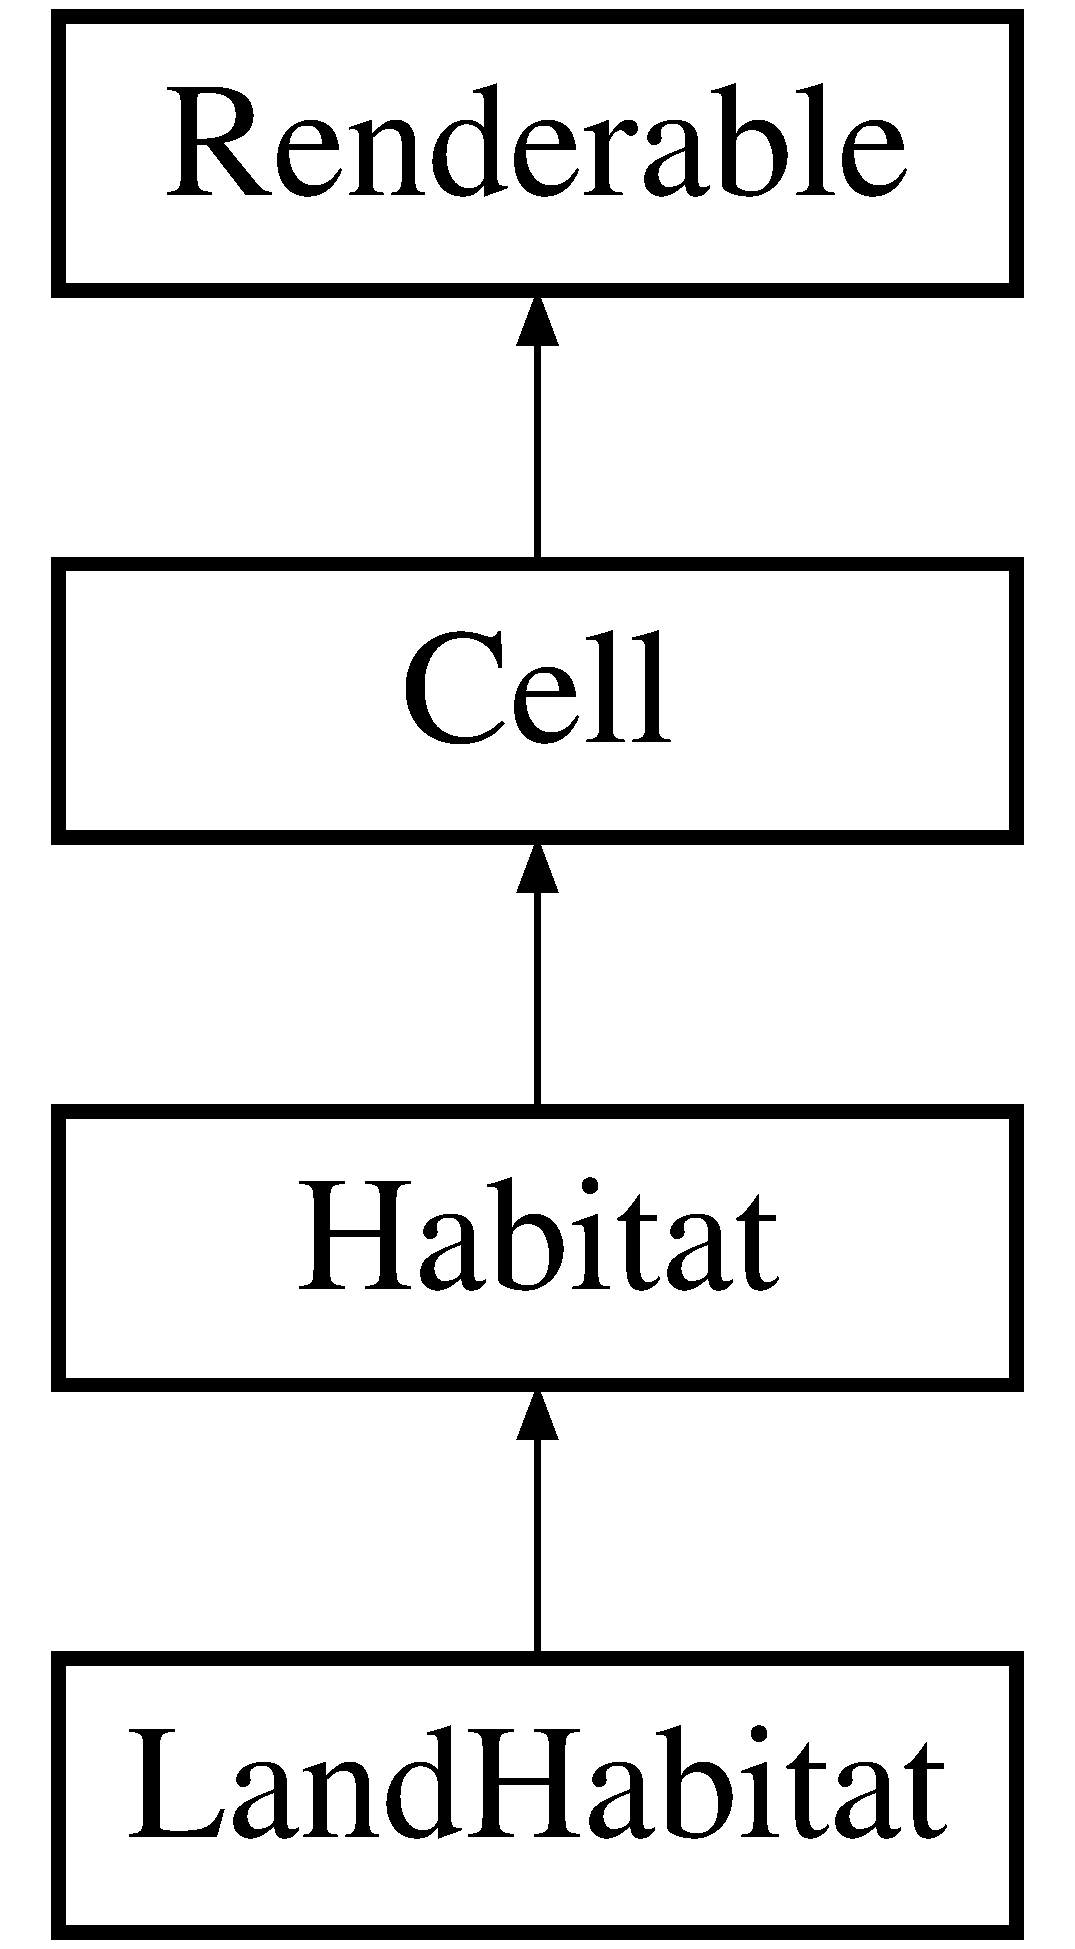
\includegraphics[height=4.000000cm]{classLandHabitat}
\end{center}
\end{figure}
\subsection*{Public Member Functions}
\begin{DoxyCompactItemize}
\item 
\hypertarget{classLandHabitat_afa67ffdf6984ec7c1fcc6ec27d5628d3}{\hyperlink{classLandHabitat_afa67ffdf6984ec7c1fcc6ec27d5628d3}{Land\+Habitat} ()}\label{classLandHabitat_afa67ffdf6984ec7c1fcc6ec27d5628d3}

\begin{DoxyCompactList}\small\item\em Constructor. Menciptakan sebuah \hyperlink{classLandHabitat}{Land\+Habitat}. \end{DoxyCompactList}\item 
\hypertarget{classLandHabitat_a0c1aebc080f875b9053f3a776aea627a}{virtual \hyperlink{classLandHabitat_a0c1aebc080f875b9053f3a776aea627a}{$\sim$\+Land\+Habitat} ()}\label{classLandHabitat_a0c1aebc080f875b9053f3a776aea627a}

\begin{DoxyCompactList}\small\item\em Destructor. \end{DoxyCompactList}\item 
\hypertarget{classLandHabitat_ad90a2fd22fa5b521d5e19e61798e3175}{void \hyperlink{classLandHabitat_ad90a2fd22fa5b521d5e19e61798e3175}{render} ()}\label{classLandHabitat_ad90a2fd22fa5b521d5e19e61798e3175}

\begin{DoxyCompactList}\small\item\em Menampilkan \hyperlink{classLandHabitat}{Land\+Habitat} ke console teks. \end{DoxyCompactList}\end{DoxyCompactItemize}
\subsection*{Additional Inherited Members}


\subsection{Detailed Description}
Kelas \hyperlink{classLandHabitat}{Land\+Habitat} yang merepesentasikan habitat untuk hewan darat. 

The documentation for this class was generated from the following files\+:\begin{DoxyCompactItemize}
\item 
src/\+Cell/\+Habitat/\+Land\+Habitat/Land\+Habitat.\+h\item 
src/\+Cell/\+Habitat/\+Land\+Habitat/Land\+Habitat.\+cpp\end{DoxyCompactItemize}

\hypertarget{classLeopard}{\section{Leopard Class Reference}
\label{classLeopard}\index{Leopard@{Leopard}}
}


{\ttfamily \#include $<$Leopard.\+h$>$}

Inheritance diagram for Leopard\+:\begin{figure}[H]
\begin{center}
\leavevmode
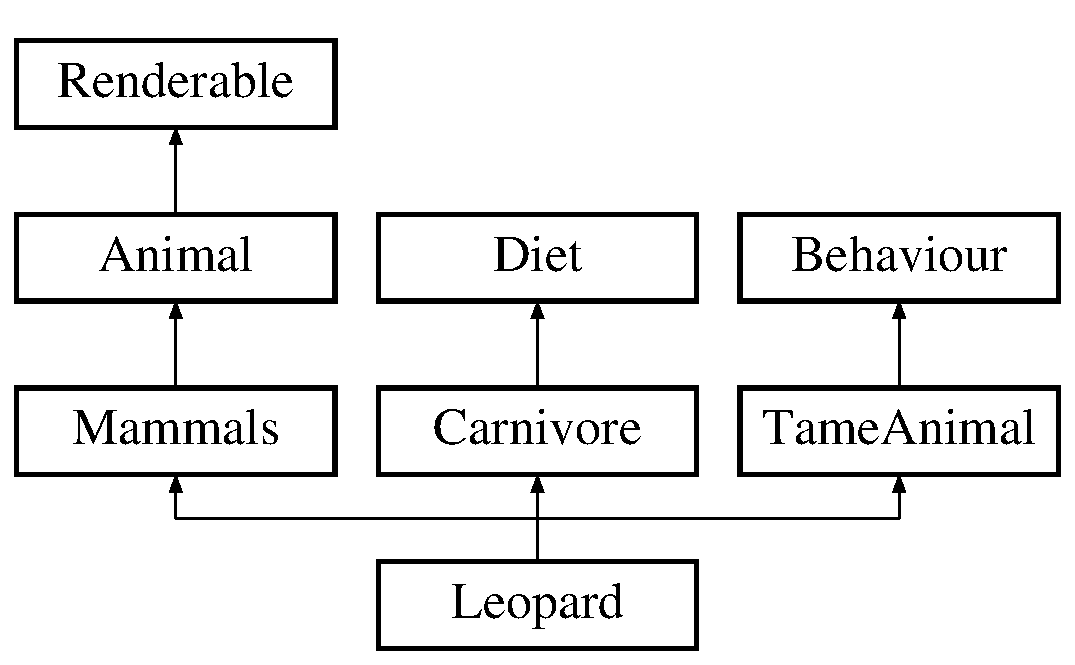
\includegraphics[height=4.000000cm]{classLeopard}
\end{center}
\end{figure}
\subsection*{Public Member Functions}
\begin{DoxyCompactItemize}
\item 
\hypertarget{classLeopard_a61dec30839864695de1c7a865fee2c0b}{\hyperlink{classLeopard_a61dec30839864695de1c7a865fee2c0b}{Leopard} (int \+\_\+weight)}\label{classLeopard_a61dec30839864695de1c7a865fee2c0b}

\begin{DoxyCompactList}\small\item\em Constructor. Menciptakan macan tutul. \end{DoxyCompactList}\item 
string \hyperlink{classLeopard_a8f74bdd86e8df25bbab7d1136944e7d9}{interact} () const 
\begin{DoxyCompactList}\small\item\em Melakukan interaksi dengan macan tutul. \end{DoxyCompactList}\end{DoxyCompactItemize}
\subsection*{Additional Inherited Members}


\subsection{Detailed Description}
Kelas \hyperlink{classLeopard}{Leopard} yang merepesentasikan macan tutul. 

\subsection{Member Function Documentation}
\hypertarget{classLeopard_a8f74bdd86e8df25bbab7d1136944e7d9}{\index{Leopard@{Leopard}!interact@{interact}}
\index{interact@{interact}!Leopard@{Leopard}}
\subsubsection[{interact}]{\setlength{\rightskip}{0pt plus 5cm}string Leopard\+::interact (
\begin{DoxyParamCaption}
{}
\end{DoxyParamCaption}
) const}}\label{classLeopard_a8f74bdd86e8df25bbab7d1136944e7d9}


Melakukan interaksi dengan macan tutul. 

\begin{DoxyReturn}{Returns}
Experience yang dirasakan ketika berinteraksi dengan macan tutul. 
\end{DoxyReturn}


The documentation for this class was generated from the following files\+:\begin{DoxyCompactItemize}
\item 
src/\+Animal/\+Mammals/\+Leopard/Leopard.\+h\item 
src/\+Animal/\+Mammals/\+Leopard/Leopard.\+cpp\end{DoxyCompactItemize}

\hypertarget{classLion}{\section{Lion Class Reference}
\label{classLion}\index{Lion@{Lion}}
}


{\ttfamily \#include $<$Lion.\+h$>$}

Inheritance diagram for Lion\+:\begin{figure}[H]
\begin{center}
\leavevmode
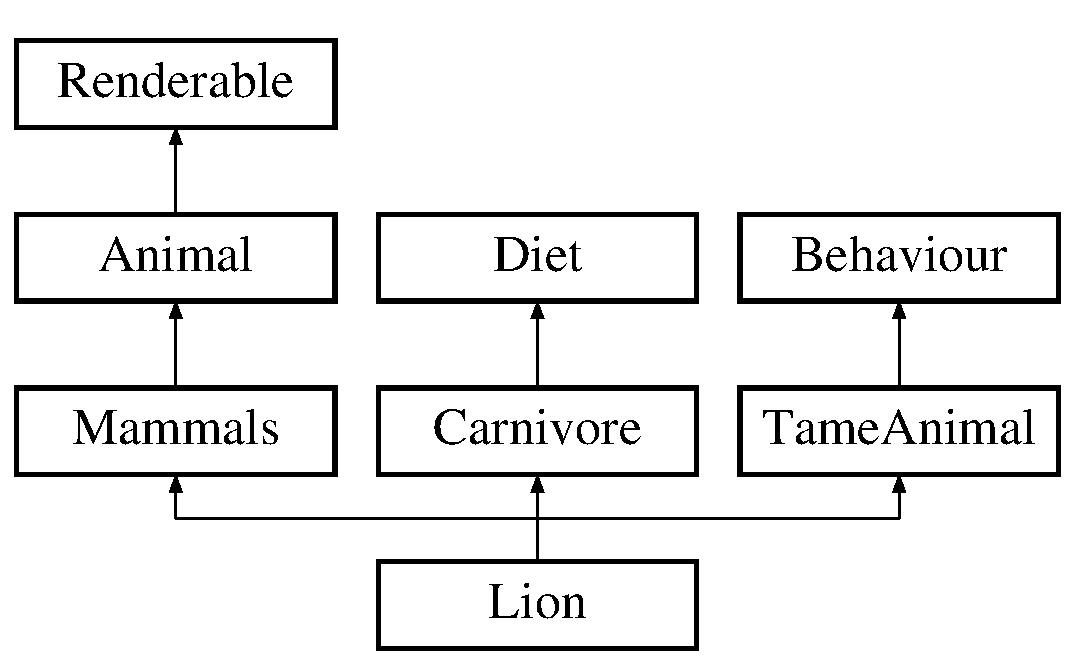
\includegraphics[height=4.000000cm]{classLion}
\end{center}
\end{figure}
\subsection*{Public Member Functions}
\begin{DoxyCompactItemize}
\item 
\hypertarget{classLion_ab3f1740ebe2231032526f410fee4d14c}{\hyperlink{classLion_ab3f1740ebe2231032526f410fee4d14c}{Lion} (int \+\_\+weight)}\label{classLion_ab3f1740ebe2231032526f410fee4d14c}

\begin{DoxyCompactList}\small\item\em Constructor. Menciptakan singa. \end{DoxyCompactList}\item 
string \hyperlink{classLion_ae05ecf4aed9b949f855bec4285c96600}{interact} () const 
\begin{DoxyCompactList}\small\item\em Melakukan interaksi dengan \hyperlink{classLion}{Lion}. \end{DoxyCompactList}\end{DoxyCompactItemize}
\subsection*{Additional Inherited Members}


\subsection{Detailed Description}
Kelas \hyperlink{classLion}{Lion} yang merepesentasikan singa. 

\subsection{Member Function Documentation}
\hypertarget{classLion_ae05ecf4aed9b949f855bec4285c96600}{\index{Lion@{Lion}!interact@{interact}}
\index{interact@{interact}!Lion@{Lion}}
\subsubsection[{interact}]{\setlength{\rightskip}{0pt plus 5cm}string Lion\+::interact (
\begin{DoxyParamCaption}
{}
\end{DoxyParamCaption}
) const}}\label{classLion_ae05ecf4aed9b949f855bec4285c96600}


Melakukan interaksi dengan \hyperlink{classLion}{Lion}. 

\begin{DoxyReturn}{Returns}
Experience yang dirasakan ketika berinteraksi dengan singa. 
\end{DoxyReturn}


The documentation for this class was generated from the following files\+:\begin{DoxyCompactItemize}
\item 
src/\+Animal/\+Mammals/\+Lion/Lion.\+h\item 
src/\+Animal/\+Mammals/\+Lion/Lion.\+cpp\end{DoxyCompactItemize}

\hypertarget{classLionfish}{\section{Lionfish Class Reference}
\label{classLionfish}\index{Lionfish@{Lionfish}}
}


{\ttfamily \#include $<$Lionfish.\+h$>$}

Inheritance diagram for Lionfish\+:\begin{figure}[H]
\begin{center}
\leavevmode
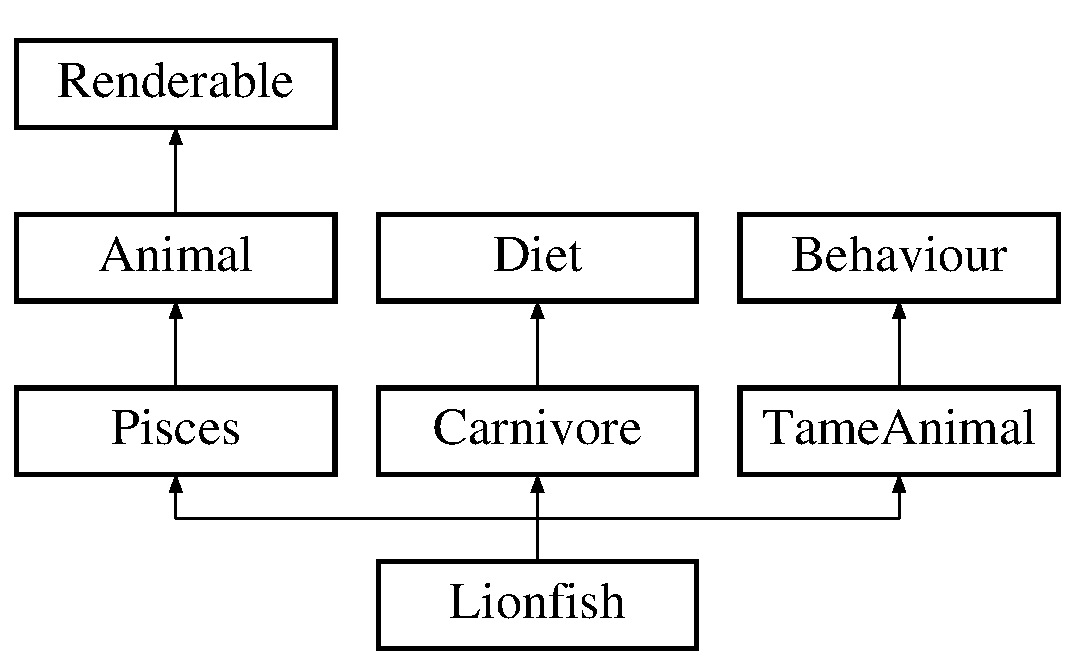
\includegraphics[height=4.000000cm]{classLionfish}
\end{center}
\end{figure}
\subsection*{Public Member Functions}
\begin{DoxyCompactItemize}
\item 
\hypertarget{classLionfish_ad6ddd21f4697048c5ba38dbfbdd7081d}{\hyperlink{classLionfish_ad6ddd21f4697048c5ba38dbfbdd7081d}{Lionfish} (int \+\_\+weight)}\label{classLionfish_ad6ddd21f4697048c5ba38dbfbdd7081d}

\begin{DoxyCompactList}\small\item\em Constructor. Menciptakan lionfish. \end{DoxyCompactList}\item 
string \hyperlink{classLionfish_aa5bdb90e93360ae9e9e2fda9a6480c5d}{interact} () const 
\begin{DoxyCompactList}\small\item\em Melakukan interaksi dengan lionfish. \end{DoxyCompactList}\end{DoxyCompactItemize}
\subsection*{Additional Inherited Members}


\subsection{Detailed Description}
Kelas \hyperlink{classLionfish}{Lionfish} yang merepesentasikan lionfish. 

\subsection{Member Function Documentation}
\hypertarget{classLionfish_aa5bdb90e93360ae9e9e2fda9a6480c5d}{\index{Lionfish@{Lionfish}!interact@{interact}}
\index{interact@{interact}!Lionfish@{Lionfish}}
\subsubsection[{interact}]{\setlength{\rightskip}{0pt plus 5cm}string Lionfish\+::interact (
\begin{DoxyParamCaption}
{}
\end{DoxyParamCaption}
) const}}\label{classLionfish_aa5bdb90e93360ae9e9e2fda9a6480c5d}


Melakukan interaksi dengan lionfish. 

\begin{DoxyReturn}{Returns}
Experience yang dirasakan ketika berinteraksi dengan lionfish. 
\end{DoxyReturn}


The documentation for this class was generated from the following files\+:\begin{DoxyCompactItemize}
\item 
src/\+Animal/\+Pisces/\+Lionfish/Lionfish.\+h\item 
src/\+Animal/\+Pisces/\+Lionfish/Lionfish.\+cpp\end{DoxyCompactItemize}

\hypertarget{classMammals}{\section{Mammals Class Reference}
\label{classMammals}\index{Mammals@{Mammals}}
}


{\ttfamily \#include $<$Mammals.\+h$>$}

Inheritance diagram for Mammals\+:\begin{figure}[H]
\begin{center}
\leavevmode
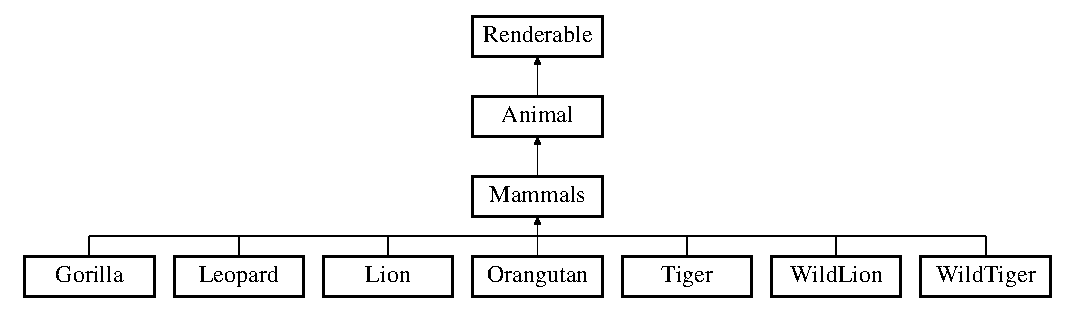
\includegraphics[height=3.764706cm]{classMammals}
\end{center}
\end{figure}
\subsection*{Public Member Functions}
\begin{DoxyCompactItemize}
\item 
\hyperlink{classMammals_a039a67cdea1502873661ec2fa55e13d5}{Mammals} (const string \&name)
\begin{DoxyCompactList}\small\item\em Constructor. Menciptakan Mamalia yang memiliki skin\+Type \char`\"{}\+Fur\char`\"{} dan reproduction \char`\"{}\+Vivipar\char`\"{}. \end{DoxyCompactList}\end{DoxyCompactItemize}
\subsection*{Additional Inherited Members}


\subsection{Detailed Description}
Kelas abstrak \hyperlink{classMammals}{Mammals} yang merepesentasikan kelas hewan Mamalia.

Kelas abstrak \hyperlink{classPisces}{Pisces} yang merepesentasikan kelas hewan \hyperlink{classPisces}{Pisces}. 

\subsection{Constructor \& Destructor Documentation}
\hypertarget{classMammals_a039a67cdea1502873661ec2fa55e13d5}{\index{Mammals@{Mammals}!Mammals@{Mammals}}
\index{Mammals@{Mammals}!Mammals@{Mammals}}
\subsubsection[{Mammals}]{\setlength{\rightskip}{0pt plus 5cm}Mammals\+::\+Mammals (
\begin{DoxyParamCaption}
\item[{const string \&}]{name}
\end{DoxyParamCaption}
)}}\label{classMammals_a039a67cdea1502873661ec2fa55e13d5}


Constructor. Menciptakan Mamalia yang memiliki skin\+Type \char`\"{}\+Fur\char`\"{} dan reproduction \char`\"{}\+Vivipar\char`\"{}. 

Constructor. Menciptakan \hyperlink{classMammals}{Mammals} yang memiliki skin\+Type \char`\"{}\+Fur\char`\"{} dan reproduction \char`\"{}\+Vivipar\char`\"{}.


\begin{DoxyParams}{Parameters}
{\em name} & Nama hewan \\
\hline
\end{DoxyParams}


The documentation for this class was generated from the following files\+:\begin{DoxyCompactItemize}
\item 
src/\+Animal/\+Mammals/Mammals.\+h\item 
src/\+Animal/\+Mammals/Mammals.\+cpp\end{DoxyCompactItemize}

\hypertarget{classOmnivore}{\section{Omnivore Class Reference}
\label{classOmnivore}\index{Omnivore@{Omnivore}}
}
Inheritance diagram for Omnivore\+:\begin{figure}[H]
\begin{center}
\leavevmode
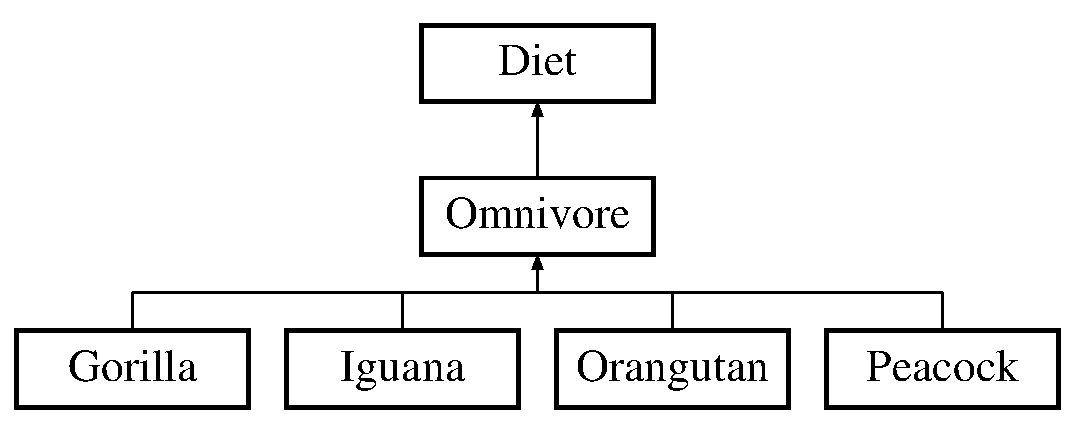
\includegraphics[height=3.000000cm]{classOmnivore}
\end{center}
\end{figure}
\subsection*{Public Member Functions}
\begin{DoxyCompactItemize}
\item 
\hyperlink{classOmnivore_a0850bb9e0327d0c63fb9961b2266a776}{Omnivore} (int \+\_\+weight, double \+\_\+ratio)
\begin{DoxyCompactList}\small\item\em Constructor. Menciptakan hewan omnivora dengan berat tertentu. \end{DoxyCompactList}\end{DoxyCompactItemize}
\subsection*{Additional Inherited Members}


\subsection{Constructor \& Destructor Documentation}
\hypertarget{classOmnivore_a0850bb9e0327d0c63fb9961b2266a776}{\index{Omnivore@{Omnivore}!Omnivore@{Omnivore}}
\index{Omnivore@{Omnivore}!Omnivore@{Omnivore}}
\subsubsection[{Omnivore}]{\setlength{\rightskip}{0pt plus 5cm}Omnivore\+::\+Omnivore (
\begin{DoxyParamCaption}
\item[{int}]{\+\_\+weight, }
\item[{double}]{\+\_\+ratio}
\end{DoxyParamCaption}
)}}\label{classOmnivore_a0850bb9e0327d0c63fb9961b2266a776}


Constructor. Menciptakan hewan omnivora dengan berat tertentu. 


\begin{DoxyParams}{Parameters}
{\em \+\_\+weight} & Berat dari hewan. \\
\hline
\end{DoxyParams}


The documentation for this class was generated from the following files\+:\begin{DoxyCompactItemize}
\item 
src/\+Animal/\+Diet/\+Omnivore/Omnivore.\+h\item 
src/\+Animal/\+Diet/\+Omnivore/Omnivore.\+cpp\end{DoxyCompactItemize}

\hypertarget{classOrangutan}{\section{Orangutan Class Reference}
\label{classOrangutan}\index{Orangutan@{Orangutan}}
}


{\ttfamily \#include $<$Orangutan.\+h$>$}

Inheritance diagram for Orangutan\+:\begin{figure}[H]
\begin{center}
\leavevmode
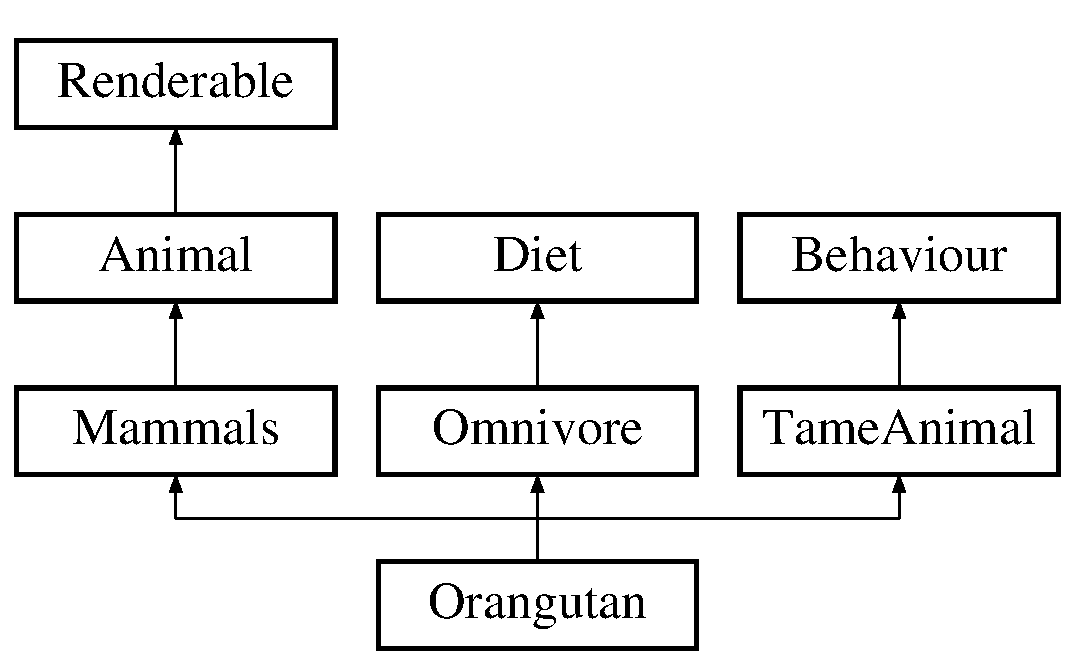
\includegraphics[height=4.000000cm]{classOrangutan}
\end{center}
\end{figure}
\subsection*{Public Member Functions}
\begin{DoxyCompactItemize}
\item 
\hypertarget{classOrangutan_a445822c4e7fa376eec207605704afae9}{\hyperlink{classOrangutan_a445822c4e7fa376eec207605704afae9}{Orangutan} (int \+\_\+weight)}\label{classOrangutan_a445822c4e7fa376eec207605704afae9}

\begin{DoxyCompactList}\small\item\em Constructor. Menciptakan orangutan. \end{DoxyCompactList}\item 
string \hyperlink{classOrangutan_a130b3521fa378e99cf78ffcf5883a7b0}{interact} () const 
\begin{DoxyCompactList}\small\item\em Melakukan interaksi dengan orangutan. \end{DoxyCompactList}\end{DoxyCompactItemize}
\subsection*{Additional Inherited Members}


\subsection{Detailed Description}
Kelas \hyperlink{classOrangutan}{Orangutan} yang merepesentasikan orangutan. 

\subsection{Member Function Documentation}
\hypertarget{classOrangutan_a130b3521fa378e99cf78ffcf5883a7b0}{\index{Orangutan@{Orangutan}!interact@{interact}}
\index{interact@{interact}!Orangutan@{Orangutan}}
\subsubsection[{interact}]{\setlength{\rightskip}{0pt plus 5cm}string Orangutan\+::interact (
\begin{DoxyParamCaption}
{}
\end{DoxyParamCaption}
) const}}\label{classOrangutan_a130b3521fa378e99cf78ffcf5883a7b0}


Melakukan interaksi dengan orangutan. 

\begin{DoxyReturn}{Returns}
Experience yang dirasakan ketika berinteraksi dengan orangutan. 
\end{DoxyReturn}


The documentation for this class was generated from the following files\+:\begin{DoxyCompactItemize}
\item 
src/\+Animal/\+Mammals/\+Orangutan/Orangutan.\+h\item 
src/\+Animal/\+Mammals/\+Orangutan/Orangutan.\+cpp\end{DoxyCompactItemize}

\hypertarget{classOwl}{\section{Owl Class Reference}
\label{classOwl}\index{Owl@{Owl}}
}


{\ttfamily \#include $<$Owl.\+h$>$}

Inheritance diagram for Owl\+:\begin{figure}[H]
\begin{center}
\leavevmode
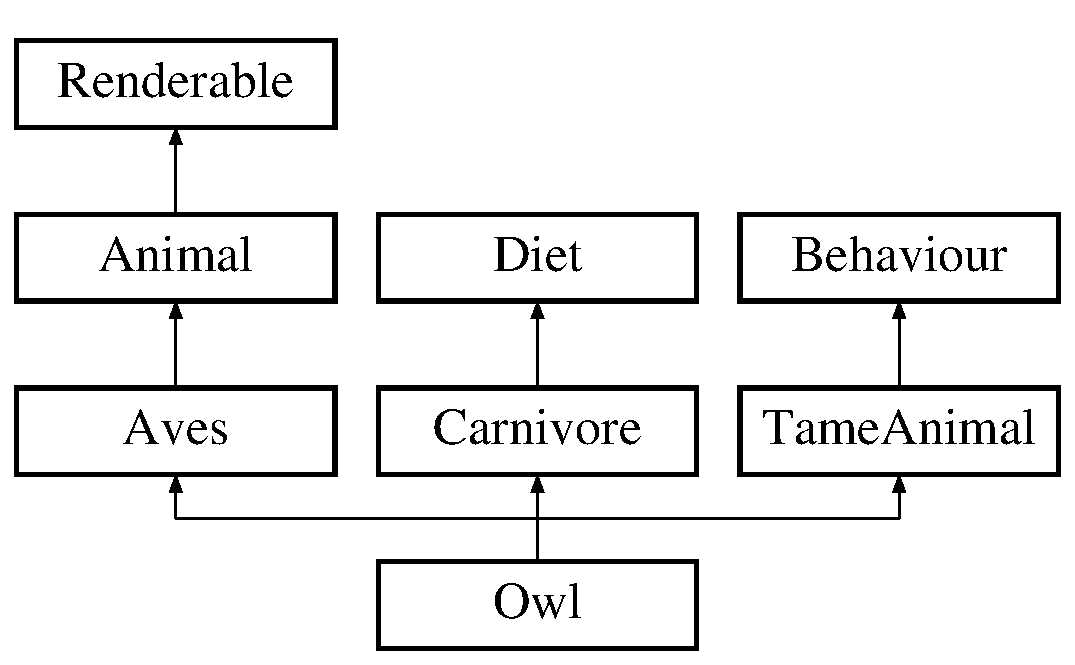
\includegraphics[height=4.000000cm]{classOwl}
\end{center}
\end{figure}
\subsection*{Public Member Functions}
\begin{DoxyCompactItemize}
\item 
\hypertarget{classOwl_adbe3753bae7d7fd91fd10705468b67c0}{\hyperlink{classOwl_adbe3753bae7d7fd91fd10705468b67c0}{Owl} (int \+\_\+weight)}\label{classOwl_adbe3753bae7d7fd91fd10705468b67c0}

\begin{DoxyCompactList}\small\item\em Constructor. Menciptakan burung hantu. \end{DoxyCompactList}\item 
string \hyperlink{classOwl_a36e657b217e4dcc09321c3740a904d22}{interact} () const 
\begin{DoxyCompactList}\small\item\em Melakukan interaksi dengan burung hantu. \end{DoxyCompactList}\end{DoxyCompactItemize}
\subsection*{Additional Inherited Members}


\subsection{Detailed Description}
Kelas \hyperlink{classOwl}{Owl} yang merepesentasikan burung hantu. 

\subsection{Member Function Documentation}
\hypertarget{classOwl_a36e657b217e4dcc09321c3740a904d22}{\index{Owl@{Owl}!interact@{interact}}
\index{interact@{interact}!Owl@{Owl}}
\subsubsection[{interact}]{\setlength{\rightskip}{0pt plus 5cm}string Owl\+::interact (
\begin{DoxyParamCaption}
{}
\end{DoxyParamCaption}
) const}}\label{classOwl_a36e657b217e4dcc09321c3740a904d22}


Melakukan interaksi dengan burung hantu. 

\begin{DoxyReturn}{Returns}
Experience yang dirasakan ketika berinteraksi dengan burung hantu. 
\end{DoxyReturn}


The documentation for this class was generated from the following files\+:\begin{DoxyCompactItemize}
\item 
src/\+Animal/\+Aves/\+Owl/Owl.\+h\item 
src/\+Animal/\+Aves/\+Owl/Owl.\+cpp\end{DoxyCompactItemize}

\hypertarget{classPark}{\section{Park Class Reference}
\label{classPark}\index{Park@{Park}}
}


{\ttfamily \#include $<$Park.\+h$>$}

Inheritance diagram for Park\+:\begin{figure}[H]
\begin{center}
\leavevmode
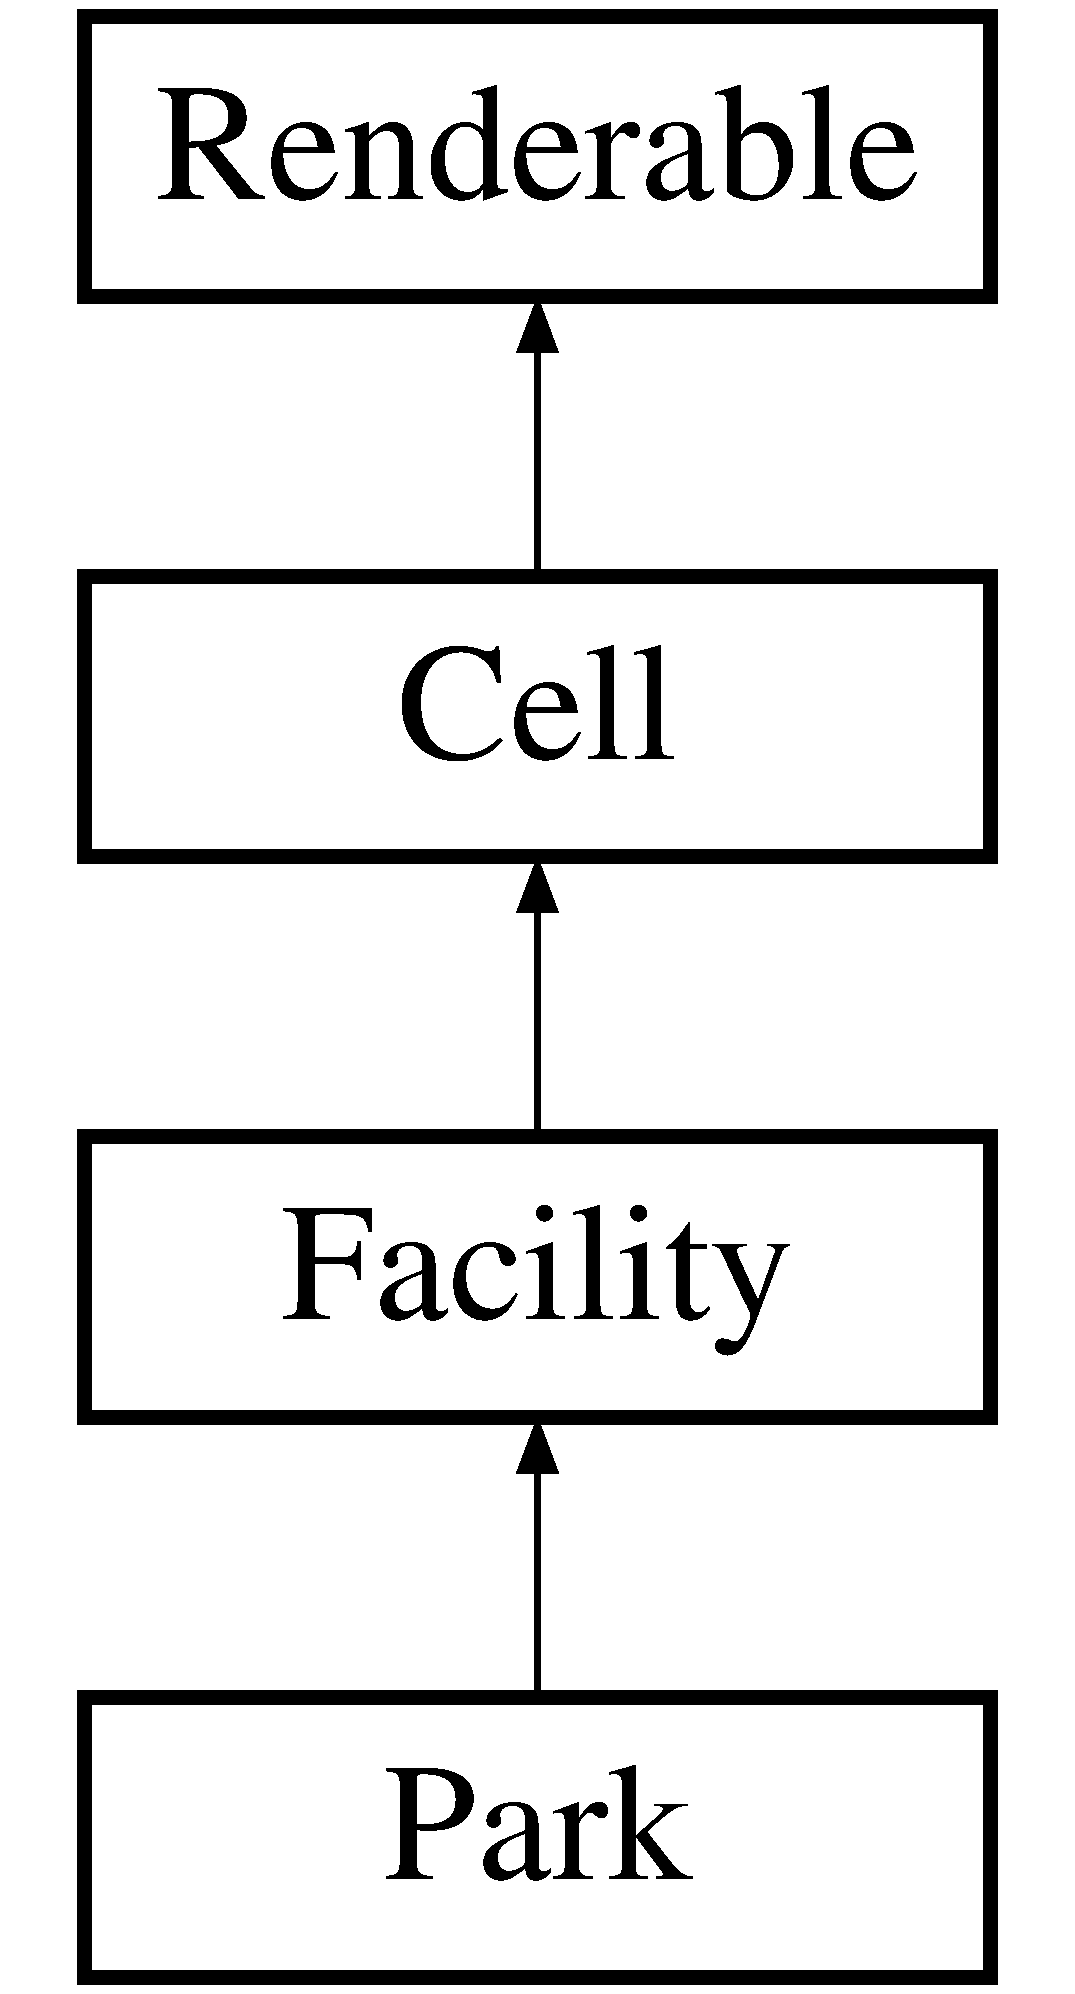
\includegraphics[height=4.000000cm]{classPark}
\end{center}
\end{figure}
\subsection*{Public Member Functions}
\begin{DoxyCompactItemize}
\item 
\hyperlink{classPark_aa7122ab2a8e5da8cd1b3c50cdbfdfec2}{Park} (bool \+\_\+accessible)
\begin{DoxyCompactList}\small\item\em Constructor. Menciptakan sebuah taman dengan status aksesibilitas tertentu. \end{DoxyCompactList}\item 
\hypertarget{classPark_aae611d70a5a38a5716cb2358a4a62c7c}{virtual \hyperlink{classPark_aae611d70a5a38a5716cb2358a4a62c7c}{$\sim$\+Park} ()}\label{classPark_aae611d70a5a38a5716cb2358a4a62c7c}

\begin{DoxyCompactList}\small\item\em Destructor. \end{DoxyCompactList}\item 
\hypertarget{classPark_afd7fe6ec511aab1b2451096b54c3addd}{void \hyperlink{classPark_afd7fe6ec511aab1b2451096b54c3addd}{render} ()}\label{classPark_afd7fe6ec511aab1b2451096b54c3addd}

\begin{DoxyCompactList}\small\item\em Menampilkan taman ke console teks. \end{DoxyCompactList}\end{DoxyCompactItemize}
\subsection*{Additional Inherited Members}


\subsection{Detailed Description}
Kelas \hyperlink{classPark}{Park} yang merepesentasikan fasilitas yang berupa taman. 

\subsection{Constructor \& Destructor Documentation}
\hypertarget{classPark_aa7122ab2a8e5da8cd1b3c50cdbfdfec2}{\index{Park@{Park}!Park@{Park}}
\index{Park@{Park}!Park@{Park}}
\subsubsection[{Park}]{\setlength{\rightskip}{0pt plus 5cm}Park\+::\+Park (
\begin{DoxyParamCaption}
\item[{bool}]{\+\_\+accessible}
\end{DoxyParamCaption}
)}}\label{classPark_aa7122ab2a8e5da8cd1b3c50cdbfdfec2}


Constructor. Menciptakan sebuah taman dengan status aksesibilitas tertentu. 


\begin{DoxyParams}{Parameters}
{\em \+\_\+accessible} & Status aksesibiltas taman. \\
\hline
\end{DoxyParams}


The documentation for this class was generated from the following files\+:\begin{DoxyCompactItemize}
\item 
src/\+Cell/\+Facility/\+Park/Park.\+h\item 
src/\+Cell/\+Facility/\+Park/Park.\+cpp\end{DoxyCompactItemize}

\hypertarget{classParrot}{\section{Parrot Class Reference}
\label{classParrot}\index{Parrot@{Parrot}}
}


{\ttfamily \#include $<$Parrot.\+h$>$}

Inheritance diagram for Parrot\+:\begin{figure}[H]
\begin{center}
\leavevmode
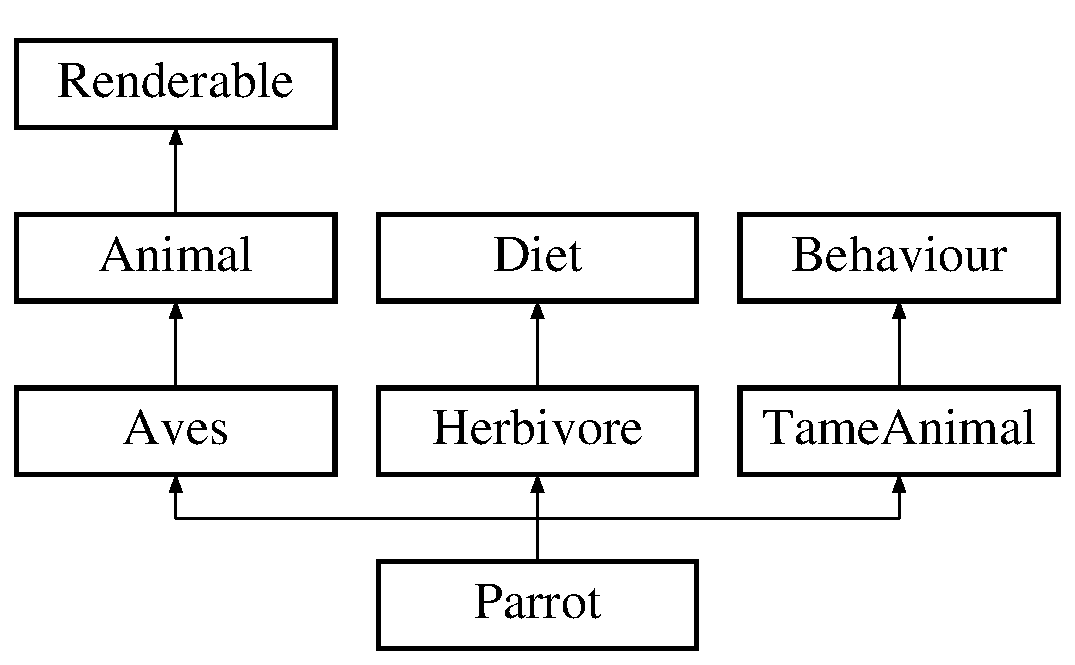
\includegraphics[height=4.000000cm]{classParrot}
\end{center}
\end{figure}
\subsection*{Additional Inherited Members}


\subsection{Detailed Description}
Kelas \hyperlink{classParrot}{Parrot} yang merepesentasikan burung beo. 

The documentation for this class was generated from the following files\+:\begin{DoxyCompactItemize}
\item 
src/\+Animal/\+Aves/\+Parrot/Parrot.\+h\item 
src/\+Animal/\+Aves/\+Parrot/Parrot.\+cpp\end{DoxyCompactItemize}

\hypertarget{classPeacock}{\section{Peacock Class Reference}
\label{classPeacock}\index{Peacock@{Peacock}}
}


{\ttfamily \#include $<$Peacock.\+h$>$}

Inheritance diagram for Peacock\+:\begin{figure}[H]
\begin{center}
\leavevmode
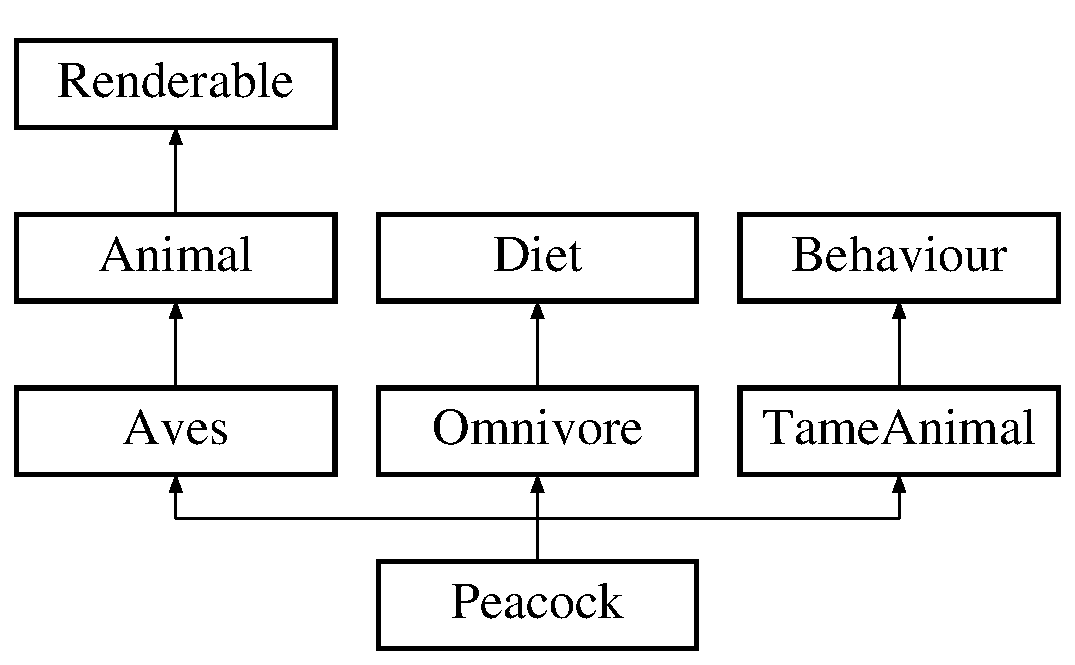
\includegraphics[height=4.000000cm]{classPeacock}
\end{center}
\end{figure}
\subsection*{Public Member Functions}
\begin{DoxyCompactItemize}
\item 
\hypertarget{classPeacock_aab6557d413568de2bcfeb74616340775}{\hyperlink{classPeacock_aab6557d413568de2bcfeb74616340775}{Peacock} (int \+\_\+weight)}\label{classPeacock_aab6557d413568de2bcfeb74616340775}

\begin{DoxyCompactList}\small\item\em Constructor. Menciptakan burung merak. \end{DoxyCompactList}\item 
string \hyperlink{classPeacock_a2d16ab89e04e3cbbef24c94181417e7f}{interact} () const 
\begin{DoxyCompactList}\small\item\em Melakukan interaksi dengan burung merak. \end{DoxyCompactList}\end{DoxyCompactItemize}
\subsection*{Additional Inherited Members}


\subsection{Detailed Description}
Kelas \hyperlink{classPeacock}{Peacock} yang merepesentasikan burung merak. 

\subsection{Member Function Documentation}
\hypertarget{classPeacock_a2d16ab89e04e3cbbef24c94181417e7f}{\index{Peacock@{Peacock}!interact@{interact}}
\index{interact@{interact}!Peacock@{Peacock}}
\subsubsection[{interact}]{\setlength{\rightskip}{0pt plus 5cm}string Peacock\+::interact (
\begin{DoxyParamCaption}
{}
\end{DoxyParamCaption}
) const}}\label{classPeacock_a2d16ab89e04e3cbbef24c94181417e7f}


Melakukan interaksi dengan burung merak. 

\begin{DoxyReturn}{Returns}
Experience yang dirasakan ketika berinteraksi dengan burung merak. 
\end{DoxyReturn}


The documentation for this class was generated from the following files\+:\begin{DoxyCompactItemize}
\item 
src/\+Animal/\+Aves/\+Peacock/Peacock.\+h\item 
src/\+Animal/\+Aves/\+Peacock/Peacock.\+cpp\end{DoxyCompactItemize}

\hypertarget{classPigeon}{\section{Pigeon Class Reference}
\label{classPigeon}\index{Pigeon@{Pigeon}}
}


{\ttfamily \#include $<$Pigeon.\+h$>$}

Inheritance diagram for Pigeon\+:\begin{figure}[H]
\begin{center}
\leavevmode
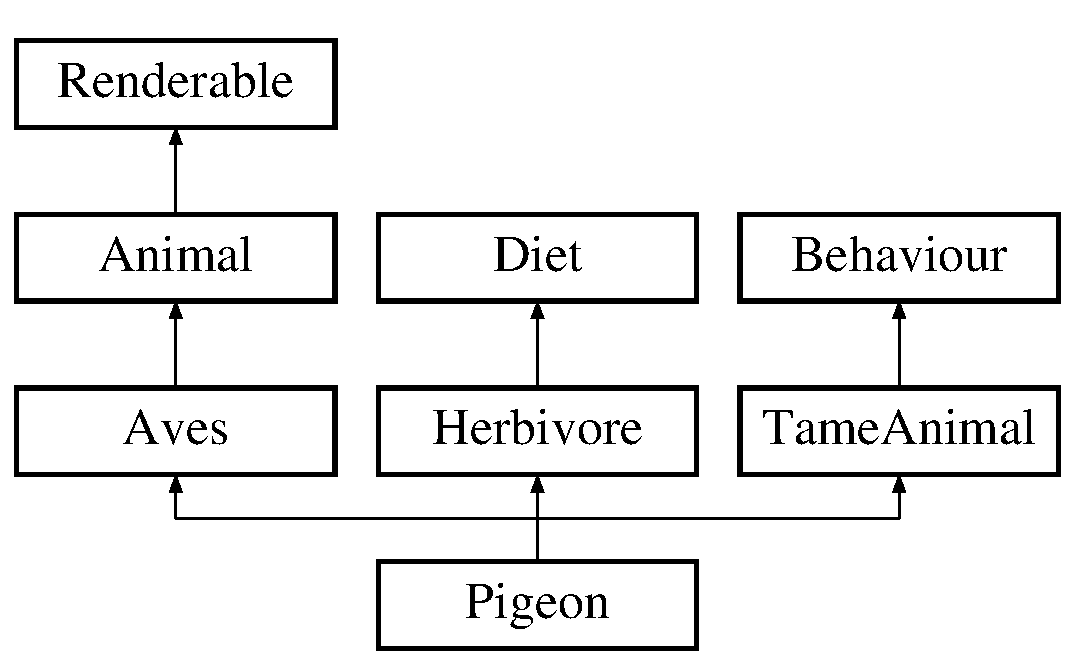
\includegraphics[height=4.000000cm]{classPigeon}
\end{center}
\end{figure}
\subsection*{Public Member Functions}
\begin{DoxyCompactItemize}
\item 
\hypertarget{classPigeon_afd6a1821b454a7b9e9e9578361e094f9}{\hyperlink{classPigeon_afd6a1821b454a7b9e9e9578361e094f9}{Pigeon} (int \+\_\+weight)}\label{classPigeon_afd6a1821b454a7b9e9e9578361e094f9}

\begin{DoxyCompactList}\small\item\em Constructor. Menciptakan burung merpati. \end{DoxyCompactList}\item 
string \hyperlink{classPigeon_afc660fc41d2ff1705be7f8751d644730}{interact} () const 
\begin{DoxyCompactList}\small\item\em Melakukan interaksi dengan burung merpati. \end{DoxyCompactList}\end{DoxyCompactItemize}
\subsection*{Additional Inherited Members}


\subsection{Detailed Description}
Kelas \hyperlink{classPigeon}{Pigeon} yang merepesentasikan burung merpati. 

\subsection{Member Function Documentation}
\hypertarget{classPigeon_afc660fc41d2ff1705be7f8751d644730}{\index{Pigeon@{Pigeon}!interact@{interact}}
\index{interact@{interact}!Pigeon@{Pigeon}}
\subsubsection[{interact}]{\setlength{\rightskip}{0pt plus 5cm}string Pigeon\+::interact (
\begin{DoxyParamCaption}
{}
\end{DoxyParamCaption}
) const}}\label{classPigeon_afc660fc41d2ff1705be7f8751d644730}


Melakukan interaksi dengan burung merpati. 

\begin{DoxyReturn}{Returns}
Experience yang dirasakan ketika berinteraksi dengan burung merpati. 
\end{DoxyReturn}


The documentation for this class was generated from the following files\+:\begin{DoxyCompactItemize}
\item 
src/\+Animal/\+Aves/\+Pigeon/Pigeon.\+h\item 
src/\+Animal/\+Aves/\+Pigeon/Pigeon.\+cpp\end{DoxyCompactItemize}

\hypertarget{classPisces}{\section{Pisces Class Reference}
\label{classPisces}\index{Pisces@{Pisces}}
}
Inheritance diagram for Pisces\+:\begin{figure}[H]
\begin{center}
\leavevmode
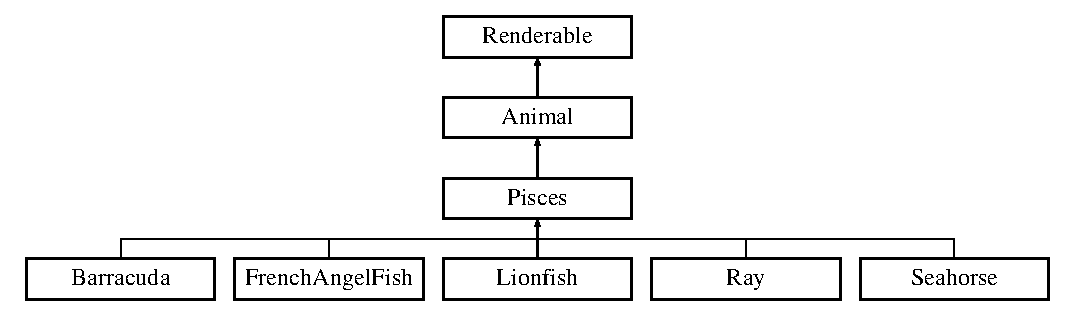
\includegraphics[height=3.796610cm]{classPisces}
\end{center}
\end{figure}
\subsection*{Public Member Functions}
\begin{DoxyCompactItemize}
\item 
\hyperlink{classPisces_a57f2e3d104a324b87a95bc86cbf6bce9}{Pisces} (const string \&name)
\begin{DoxyCompactList}\small\item\em Constructor. Menciptakan \hyperlink{classPisces}{Pisces} yang memiliki skin\+Type \char`\"{}\+Scales\char`\"{} dan reproduction \char`\"{}\+Ovipar\char`\"{}. \end{DoxyCompactList}\end{DoxyCompactItemize}
\subsection*{Additional Inherited Members}


\subsection{Constructor \& Destructor Documentation}
\hypertarget{classPisces_a57f2e3d104a324b87a95bc86cbf6bce9}{\index{Pisces@{Pisces}!Pisces@{Pisces}}
\index{Pisces@{Pisces}!Pisces@{Pisces}}
\subsubsection[{Pisces}]{\setlength{\rightskip}{0pt plus 5cm}Pisces\+::\+Pisces (
\begin{DoxyParamCaption}
\item[{const string \&}]{name}
\end{DoxyParamCaption}
)}}\label{classPisces_a57f2e3d104a324b87a95bc86cbf6bce9}


Constructor. Menciptakan \hyperlink{classPisces}{Pisces} yang memiliki skin\+Type \char`\"{}\+Scales\char`\"{} dan reproduction \char`\"{}\+Ovipar\char`\"{}. 

Constructor. Menciptakan \hyperlink{classPisces}{Pisces} yang memiliki skin\+Type \char`\"{}\+Scale\char`\"{} dan reproduction \char`\"{}\+Ovipar\char`\"{}.


\begin{DoxyParams}{Parameters}
{\em name} & Nama hewan \\
\hline
\end{DoxyParams}


The documentation for this class was generated from the following files\+:\begin{DoxyCompactItemize}
\item 
src/\+Animal/\+Pisces/Pisces.\+h\item 
src/\+Animal/\+Pisces/Pisces.\+cpp\end{DoxyCompactItemize}

\hypertarget{classPoint}{\section{Point Class Reference}
\label{classPoint}\index{Point@{Point}}
}


{\ttfamily \#include $<$Point.\+h$>$}

\subsection*{Public Member Functions}
\begin{DoxyCompactItemize}
\item 
\hypertarget{classPoint_ad92f2337b839a94ce97dcdb439b4325a}{\hyperlink{classPoint_ad92f2337b839a94ce97dcdb439b4325a}{Point} ()}\label{classPoint_ad92f2337b839a94ce97dcdb439b4325a}

\begin{DoxyCompactList}\small\item\em Constructor. Menciptakan titik dengan koordinat (0, 0). \end{DoxyCompactList}\item 
\hyperlink{classPoint_a001c4958c310b248f5c26037aea38a9c}{Point} (int x, int y)
\begin{DoxyCompactList}\small\item\em Constructor. Menciptakan titik dengan koordinat (x, y). \end{DoxyCompactList}\item 
int \hyperlink{classPoint_abe622fffc8785b0c2e06cdac681b9837}{get\+X} () const 
\begin{DoxyCompactList}\small\item\em Mengambil nilai absis. \end{DoxyCompactList}\item 
int \hyperlink{classPoint_a10f31e48e2dbc22e3660ca769b8d5d65}{get\+Y} () const 
\begin{DoxyCompactList}\small\item\em Mengambil nilai ordinat. \end{DoxyCompactList}\item 
void \hyperlink{classPoint_a89315778ce0a9175ae1a1898a93b71db}{set\+X} (int \+\_\+\+X)
\begin{DoxyCompactList}\small\item\em Set nilai absis. \end{DoxyCompactList}\item 
void \hyperlink{classPoint_a5f78572e1b8dfbace3819c3f020f3784}{set\+Y} (int \+\_\+\+Y)
\begin{DoxyCompactList}\small\item\em Set nilai ordinat. \end{DoxyCompactList}\end{DoxyCompactItemize}


\subsection{Detailed Description}
Kelas \hyperlink{classPoint}{Point} yang merepresentasikan sebuah titik. 

\subsection{Constructor \& Destructor Documentation}
\hypertarget{classPoint_a001c4958c310b248f5c26037aea38a9c}{\index{Point@{Point}!Point@{Point}}
\index{Point@{Point}!Point@{Point}}
\subsubsection[{Point}]{\setlength{\rightskip}{0pt plus 5cm}Point\+::\+Point (
\begin{DoxyParamCaption}
\item[{int}]{x, }
\item[{int}]{y}
\end{DoxyParamCaption}
)}}\label{classPoint_a001c4958c310b248f5c26037aea38a9c}


Constructor. Menciptakan titik dengan koordinat (x, y). 


\begin{DoxyParams}{Parameters}
{\em x} & Nilai absis. \\
\hline
{\em y} & Nilai ordinat. \\
\hline
\end{DoxyParams}


\subsection{Member Function Documentation}
\hypertarget{classPoint_abe622fffc8785b0c2e06cdac681b9837}{\index{Point@{Point}!get\+X@{get\+X}}
\index{get\+X@{get\+X}!Point@{Point}}
\subsubsection[{get\+X}]{\setlength{\rightskip}{0pt plus 5cm}int Point\+::get\+X (
\begin{DoxyParamCaption}
{}
\end{DoxyParamCaption}
) const}}\label{classPoint_abe622fffc8785b0c2e06cdac681b9837}


Mengambil nilai absis. 

\begin{DoxyReturn}{Returns}
Nilai absis. 
\end{DoxyReturn}
\hypertarget{classPoint_a10f31e48e2dbc22e3660ca769b8d5d65}{\index{Point@{Point}!get\+Y@{get\+Y}}
\index{get\+Y@{get\+Y}!Point@{Point}}
\subsubsection[{get\+Y}]{\setlength{\rightskip}{0pt plus 5cm}int Point\+::get\+Y (
\begin{DoxyParamCaption}
{}
\end{DoxyParamCaption}
) const}}\label{classPoint_a10f31e48e2dbc22e3660ca769b8d5d65}


Mengambil nilai ordinat. 

\begin{DoxyReturn}{Returns}
Nilai ordinat. 
\end{DoxyReturn}
\hypertarget{classPoint_a89315778ce0a9175ae1a1898a93b71db}{\index{Point@{Point}!set\+X@{set\+X}}
\index{set\+X@{set\+X}!Point@{Point}}
\subsubsection[{set\+X}]{\setlength{\rightskip}{0pt plus 5cm}void Point\+::set\+X (
\begin{DoxyParamCaption}
\item[{int}]{\+\_\+\+X}
\end{DoxyParamCaption}
)}}\label{classPoint_a89315778ce0a9175ae1a1898a93b71db}


Set nilai absis. 


\begin{DoxyParams}{Parameters}
{\em \+\_\+\+X} & Nilai absis. \\
\hline
\end{DoxyParams}
\hypertarget{classPoint_a5f78572e1b8dfbace3819c3f020f3784}{\index{Point@{Point}!set\+Y@{set\+Y}}
\index{set\+Y@{set\+Y}!Point@{Point}}
\subsubsection[{set\+Y}]{\setlength{\rightskip}{0pt plus 5cm}void Point\+::set\+Y (
\begin{DoxyParamCaption}
\item[{int}]{\+\_\+\+Y}
\end{DoxyParamCaption}
)}}\label{classPoint_a5f78572e1b8dfbace3819c3f020f3784}


Set nilai ordinat. 


\begin{DoxyParams}{Parameters}
{\em \+\_\+\+Y} & Nilai ordinat. \\
\hline
\end{DoxyParams}


The documentation for this class was generated from the following files\+:\begin{DoxyCompactItemize}
\item 
src/\+Point/Point.\+h\item 
src/\+Point/Point.\+cpp\end{DoxyCompactItemize}

\hypertarget{classPython}{\section{Python Class Reference}
\label{classPython}\index{Python@{Python}}
}


{\ttfamily \#include $<$Python.\+h$>$}

Inheritance diagram for Python\+:\begin{figure}[H]
\begin{center}
\leavevmode
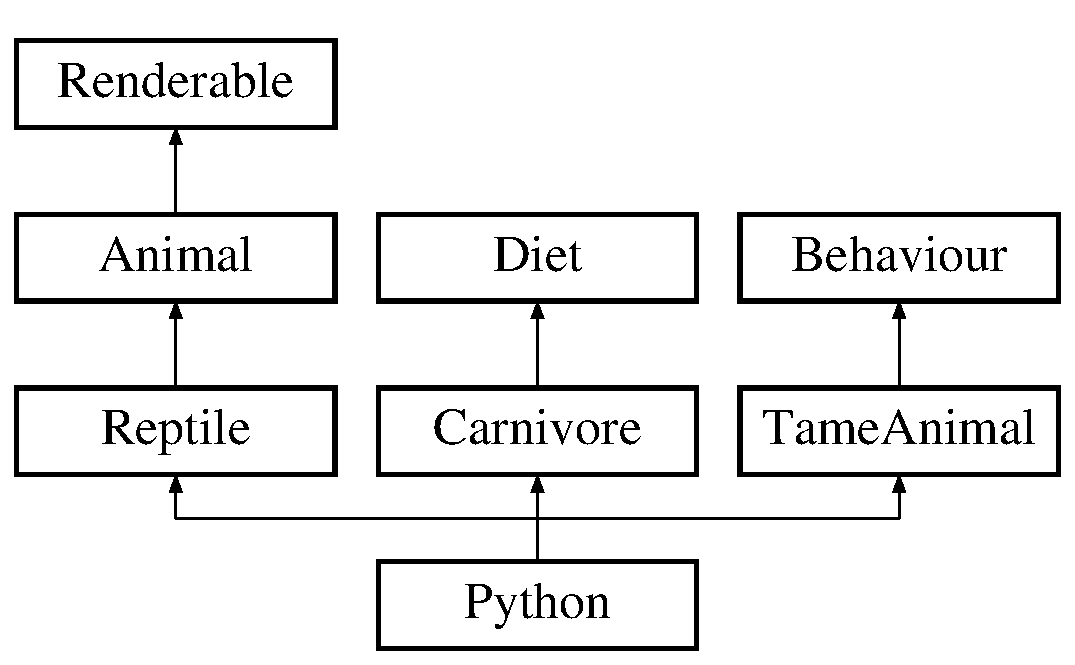
\includegraphics[height=4.000000cm]{classPython}
\end{center}
\end{figure}
\subsection*{Public Member Functions}
\begin{DoxyCompactItemize}
\item 
\hypertarget{classPython_a409f3fffc3c217bf9794c9302d15ad7d}{\hyperlink{classPython_a409f3fffc3c217bf9794c9302d15ad7d}{Python} (int \+\_\+weight)}\label{classPython_a409f3fffc3c217bf9794c9302d15ad7d}

\begin{DoxyCompactList}\small\item\em Constructor. Menciptakan ular piton. \end{DoxyCompactList}\item 
string \hyperlink{classPython_a3eeadfb5db50b6332a36962a2c3fef8a}{interact} () const 
\begin{DoxyCompactList}\small\item\em Melakukan interaksi dengan ular piton. \end{DoxyCompactList}\end{DoxyCompactItemize}
\subsection*{Additional Inherited Members}


\subsection{Detailed Description}
Kelas \hyperlink{classPython}{Python} yang merepesentasikan ular piton. 

\subsection{Member Function Documentation}
\hypertarget{classPython_a3eeadfb5db50b6332a36962a2c3fef8a}{\index{Python@{Python}!interact@{interact}}
\index{interact@{interact}!Python@{Python}}
\subsubsection[{interact}]{\setlength{\rightskip}{0pt plus 5cm}string Python\+::interact (
\begin{DoxyParamCaption}
{}
\end{DoxyParamCaption}
) const}}\label{classPython_a3eeadfb5db50b6332a36962a2c3fef8a}


Melakukan interaksi dengan ular piton. 

\begin{DoxyReturn}{Returns}
Experience yang dirasakan ketika berinteraksi dengan ular piton. 
\end{DoxyReturn}


The documentation for this class was generated from the following files\+:\begin{DoxyCompactItemize}
\item 
src/\+Animal/\+Reptile/\+Python/Python.\+h\item 
src/\+Animal/\+Reptile/\+Python/Python.\+cpp\end{DoxyCompactItemize}

\hypertarget{classRay}{\section{Ray Class Reference}
\label{classRay}\index{Ray@{Ray}}
}


{\ttfamily \#include $<$Ray.\+h$>$}

Inheritance diagram for Ray\+:\begin{figure}[H]
\begin{center}
\leavevmode
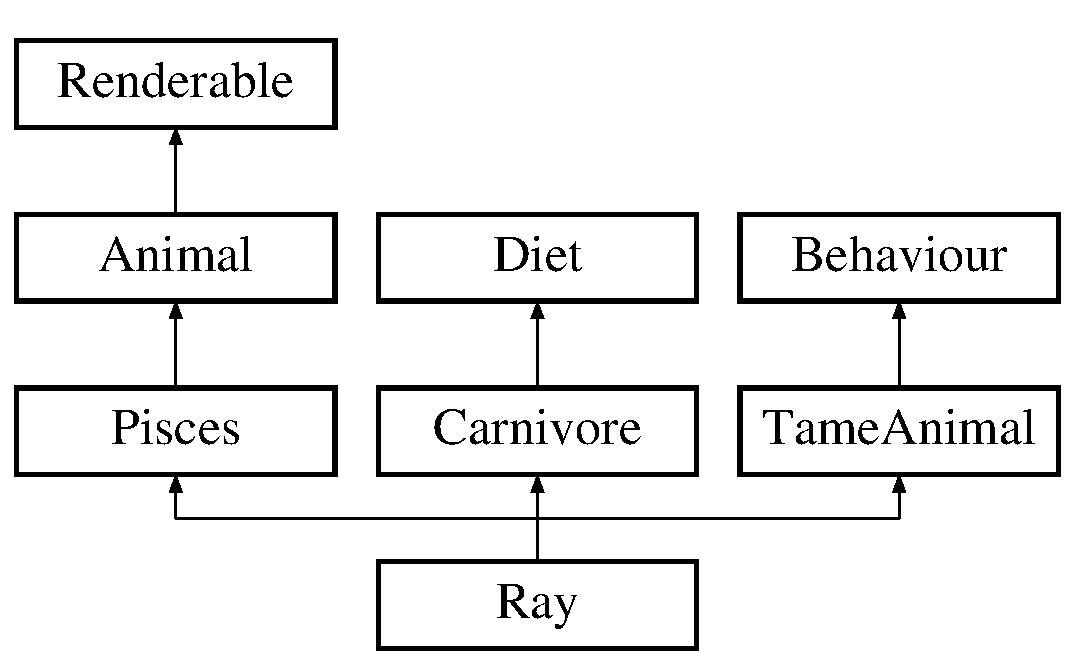
\includegraphics[height=4.000000cm]{classRay}
\end{center}
\end{figure}
\subsection*{Public Member Functions}
\begin{DoxyCompactItemize}
\item 
\hypertarget{classRay_a3ad18fbb8b6f65fff3e9b40ca829d3a6}{\hyperlink{classRay_a3ad18fbb8b6f65fff3e9b40ca829d3a6}{Ray} (int \+\_\+weight)}\label{classRay_a3ad18fbb8b6f65fff3e9b40ca829d3a6}

\begin{DoxyCompactList}\small\item\em Constructor. Menciptakan ikan pari. \end{DoxyCompactList}\item 
string \hyperlink{classRay_a4f0ad22f7378e085613d3c2289d558aa}{interact} () const 
\begin{DoxyCompactList}\small\item\em Melakukan interaksi dengan ikan pari. \end{DoxyCompactList}\end{DoxyCompactItemize}
\subsection*{Additional Inherited Members}


\subsection{Detailed Description}
Kelas \hyperlink{classRay}{Ray} yang merepesentasikan ikan pari. 

\subsection{Member Function Documentation}
\hypertarget{classRay_a4f0ad22f7378e085613d3c2289d558aa}{\index{Ray@{Ray}!interact@{interact}}
\index{interact@{interact}!Ray@{Ray}}
\subsubsection[{interact}]{\setlength{\rightskip}{0pt plus 5cm}string Ray\+::interact (
\begin{DoxyParamCaption}
{}
\end{DoxyParamCaption}
) const}}\label{classRay_a4f0ad22f7378e085613d3c2289d558aa}


Melakukan interaksi dengan ikan pari. 

\begin{DoxyReturn}{Returns}
Experience yang dirasakan ketika berinteraksi dengan ikan pari. 
\end{DoxyReturn}


The documentation for this class was generated from the following files\+:\begin{DoxyCompactItemize}
\item 
src/\+Animal/\+Pisces/\+Ray/Ray.\+h\item 
src/\+Animal/\+Pisces/\+Ray/Ray.\+cpp\end{DoxyCompactItemize}

\hypertarget{classRenderable}{\section{Renderable Class Reference}
\label{classRenderable}\index{Renderable@{Renderable}}
}


{\ttfamily \#include $<$Renderable.\+h$>$}

Inheritance diagram for Renderable\+:\begin{figure}[H]
\begin{center}
\leavevmode
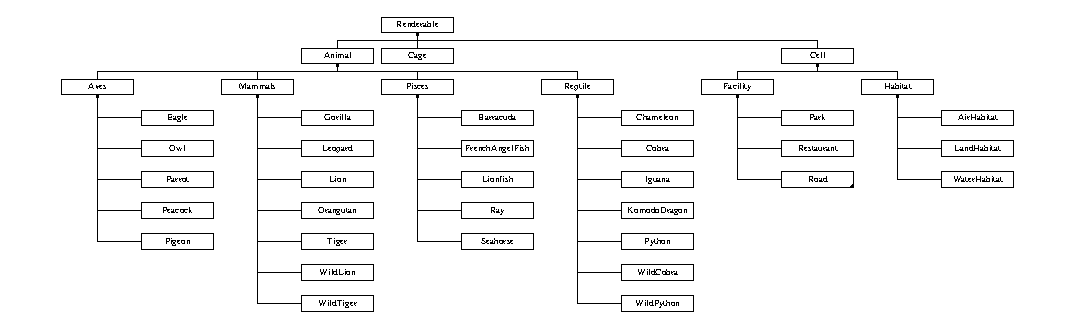
\includegraphics[height=3.954802cm]{classRenderable}
\end{center}
\end{figure}
\subsection*{Public Member Functions}
\begin{DoxyCompactItemize}
\item 
\hypertarget{classRenderable_a7d02709d871bd2bde97d41d933df5adf}{virtual void \hyperlink{classRenderable_a7d02709d871bd2bde97d41d933df5adf}{render} ()=0}\label{classRenderable_a7d02709d871bd2bde97d41d933df5adf}

\begin{DoxyCompactList}\small\item\em Mengembalikan satu karakter yang merepesentasikan bentuk objek yang bersangkutan di atas console teks. Merupakan pure virtual function. \end{DoxyCompactList}\item 
\hypertarget{classRenderable_af0e3e758db2aad1d0d874fc98736614f}{virtual int \hyperlink{classRenderable_af0e3e758db2aad1d0d874fc98736614f}{get\+X} () const =0}\label{classRenderable_af0e3e758db2aad1d0d874fc98736614f}

\begin{DoxyCompactList}\small\item\em Mengembalikan posisi X untuk pencetakan objek. \end{DoxyCompactList}\item 
\hypertarget{classRenderable_a6af0fc98ab82083dce18e9ea970480e0}{virtual int \hyperlink{classRenderable_a6af0fc98ab82083dce18e9ea970480e0}{get\+Y} () const =0}\label{classRenderable_a6af0fc98ab82083dce18e9ea970480e0}

\begin{DoxyCompactList}\small\item\em Mengembalikan posisi Y untuk pencetakan objek. \end{DoxyCompactList}\end{DoxyCompactItemize}


\subsection{Detailed Description}
Kelas abstrak \hyperlink{classRenderable}{Renderable} yang merepresentasikan perilaku objek yang dapat digambar di atas layar. 

The documentation for this class was generated from the following file\+:\begin{DoxyCompactItemize}
\item 
src/\+Renderable/Renderable.\+h\end{DoxyCompactItemize}

\hypertarget{classReptile}{\section{Reptile Class Reference}
\label{classReptile}\index{Reptile@{Reptile}}
}


{\ttfamily \#include $<$Reptile.\+h$>$}

Inheritance diagram for Reptile\+:\begin{figure}[H]
\begin{center}
\leavevmode
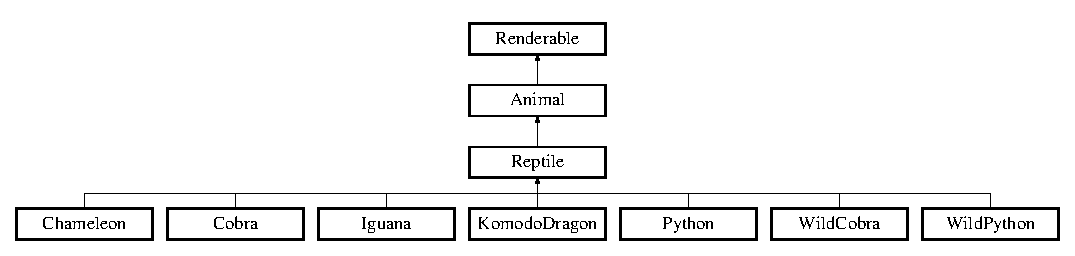
\includegraphics[height=2.990654cm]{classReptile}
\end{center}
\end{figure}
\subsection*{Public Member Functions}
\begin{DoxyCompactItemize}
\item 
\hyperlink{classReptile_aaab0ebbd70c74ada2f82f4a66a673563}{Reptile} (const string \&name)
\begin{DoxyCompactList}\small\item\em Constructor. Menciptakan Reptil yang memiliki skin\+Type \char`\"{}\+Scales\char`\"{} dan reproduction \char`\"{}\+Ovipar\char`\"{}. \end{DoxyCompactList}\end{DoxyCompactItemize}
\subsection*{Additional Inherited Members}


\subsection{Detailed Description}
Kelas abstrak \hyperlink{classReptile}{Reptile} yang merepesentasikan kelas hewan Reptil. 

\subsection{Constructor \& Destructor Documentation}
\hypertarget{classReptile_aaab0ebbd70c74ada2f82f4a66a673563}{\index{Reptile@{Reptile}!Reptile@{Reptile}}
\index{Reptile@{Reptile}!Reptile@{Reptile}}
\subsubsection[{Reptile}]{\setlength{\rightskip}{0pt plus 5cm}Reptile\+::\+Reptile (
\begin{DoxyParamCaption}
\item[{const string \&}]{name}
\end{DoxyParamCaption}
)}}\label{classReptile_aaab0ebbd70c74ada2f82f4a66a673563}


Constructor. Menciptakan Reptil yang memiliki skin\+Type \char`\"{}\+Scales\char`\"{} dan reproduction \char`\"{}\+Ovipar\char`\"{}. 


\begin{DoxyParams}{Parameters}
{\em name} & Nama hewan \\
\hline
\end{DoxyParams}


The documentation for this class was generated from the following files\+:\begin{DoxyCompactItemize}
\item 
src/\+Animal/\+Reptile/Reptile.\+h\item 
src/\+Animal/\+Reptile/Reptile.\+cpp\end{DoxyCompactItemize}

\hypertarget{classRestaurant}{\section{Restaurant Class Reference}
\label{classRestaurant}\index{Restaurant@{Restaurant}}
}


{\ttfamily \#include $<$Restaurant.\+h$>$}

Inheritance diagram for Restaurant\+:\begin{figure}[H]
\begin{center}
\leavevmode
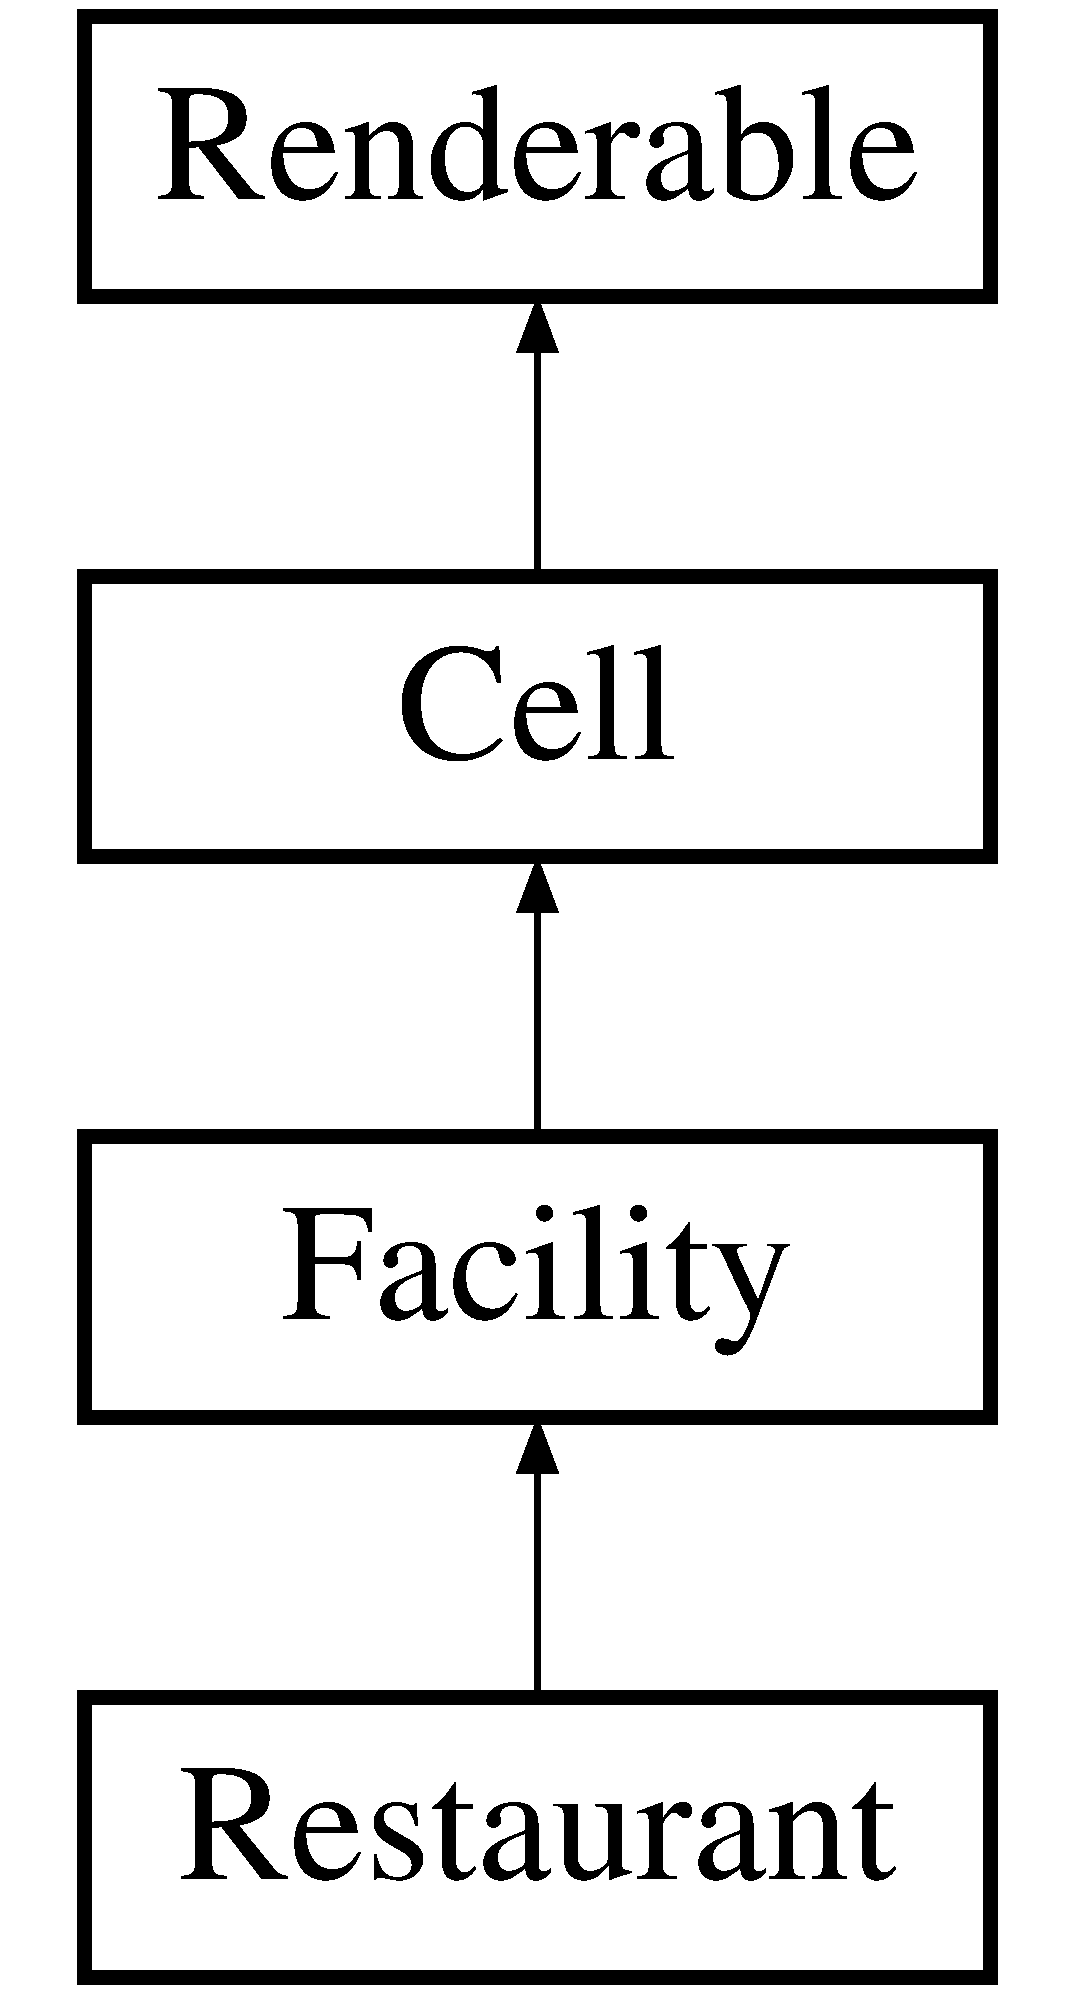
\includegraphics[height=4.000000cm]{classRestaurant}
\end{center}
\end{figure}
\subsection*{Public Member Functions}
\begin{DoxyCompactItemize}
\item 
\hyperlink{classRestaurant_a608f7988ea6a74eea642d33c05e1ee0e}{Restaurant} (bool \+\_\+accessible)
\begin{DoxyCompactList}\small\item\em Constructor. Menciptakan sebuah restoran dengan status aksesibilitas tertentu. \end{DoxyCompactList}\item 
\hypertarget{classRestaurant_acb1d786ab04bc4880e79f13d839b9cbc}{virtual \hyperlink{classRestaurant_acb1d786ab04bc4880e79f13d839b9cbc}{$\sim$\+Restaurant} ()}\label{classRestaurant_acb1d786ab04bc4880e79f13d839b9cbc}

\begin{DoxyCompactList}\small\item\em Destructor. \end{DoxyCompactList}\item 
\hypertarget{classRestaurant_a922ef15598aa096dcfe9b9903d181180}{void \hyperlink{classRestaurant_a922ef15598aa096dcfe9b9903d181180}{render} ()}\label{classRestaurant_a922ef15598aa096dcfe9b9903d181180}

\begin{DoxyCompactList}\small\item\em Menampilkan restoran ke console teks. \end{DoxyCompactList}\end{DoxyCompactItemize}
\subsection*{Additional Inherited Members}


\subsection{Detailed Description}
Kelas \hyperlink{classRestaurant}{Restaurant} yang merepesentasikan fasilitas yang berupa restoran. 

\subsection{Constructor \& Destructor Documentation}
\hypertarget{classRestaurant_a608f7988ea6a74eea642d33c05e1ee0e}{\index{Restaurant@{Restaurant}!Restaurant@{Restaurant}}
\index{Restaurant@{Restaurant}!Restaurant@{Restaurant}}
\subsubsection[{Restaurant}]{\setlength{\rightskip}{0pt plus 5cm}Restaurant\+::\+Restaurant (
\begin{DoxyParamCaption}
\item[{bool}]{\+\_\+accessible}
\end{DoxyParamCaption}
)}}\label{classRestaurant_a608f7988ea6a74eea642d33c05e1ee0e}


Constructor. Menciptakan sebuah restoran dengan status aksesibilitas tertentu. 


\begin{DoxyParams}{Parameters}
{\em \+\_\+accessible} & Status aksesibiltas restoran. \\
\hline
\end{DoxyParams}


The documentation for this class was generated from the following files\+:\begin{DoxyCompactItemize}
\item 
src/\+Cell/\+Facility/\+Restaurant/Restaurant.\+h\item 
src/\+Cell/\+Facility/\+Restaurant/Restaurant.\+cpp\end{DoxyCompactItemize}

\hypertarget{classRoad}{\section{Road Class Reference}
\label{classRoad}\index{Road@{Road}}
}


{\ttfamily \#include $<$Road.\+h$>$}

Inheritance diagram for Road\+:\begin{figure}[H]
\begin{center}
\leavevmode
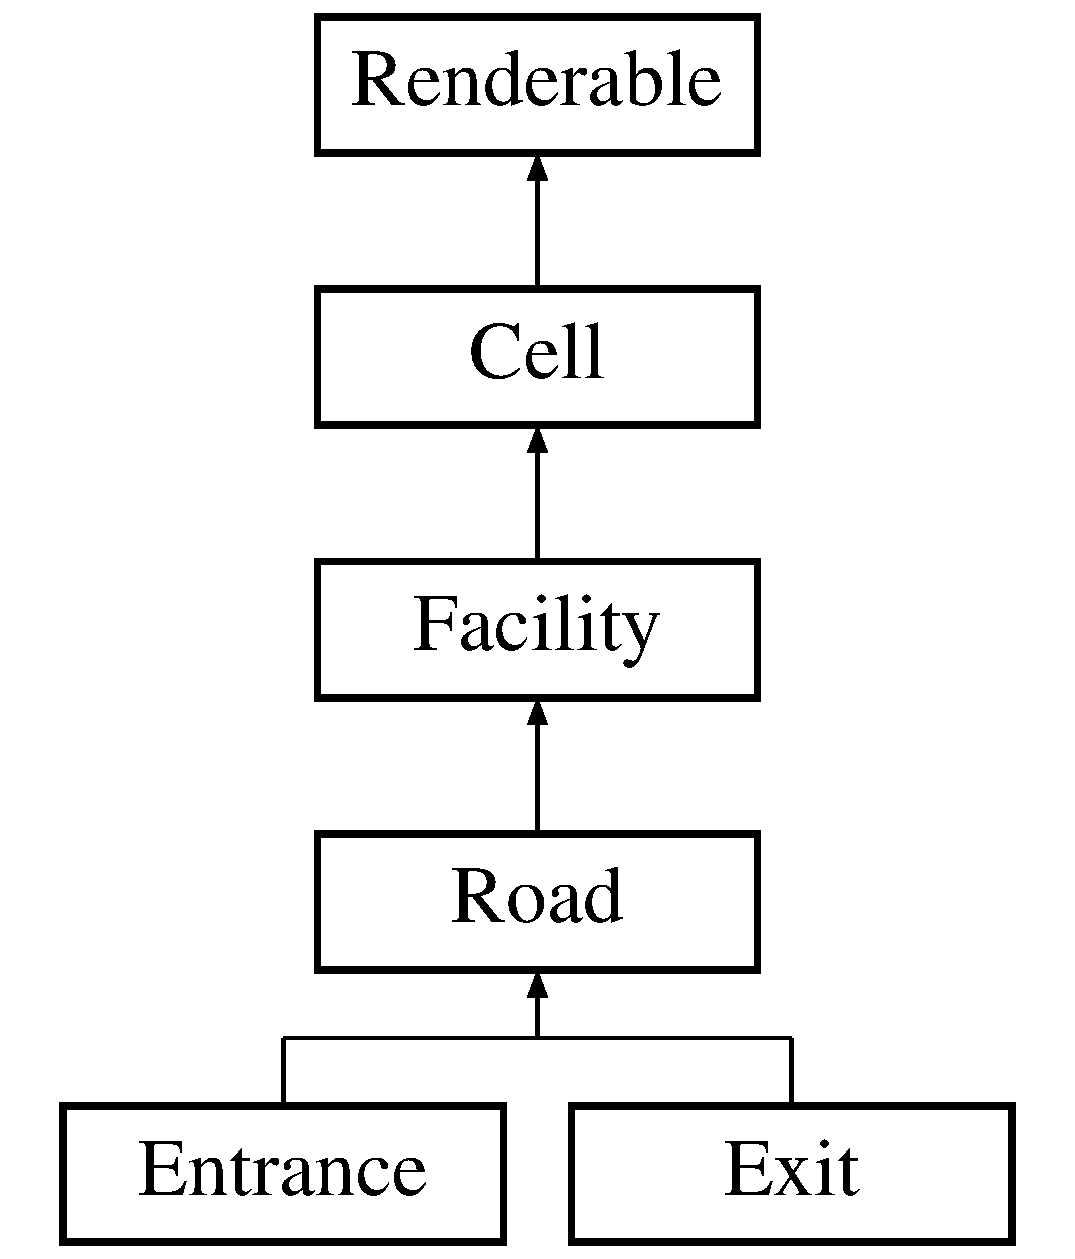
\includegraphics[height=5.000000cm]{classRoad}
\end{center}
\end{figure}
\subsection*{Public Member Functions}
\begin{DoxyCompactItemize}
\item 
\hyperlink{classRoad_ae98fca3cfb8223b281b4d7787646cf38}{Road} (bool \+\_\+accessible)
\begin{DoxyCompactList}\small\item\em Constructor. Menciptakan sebuah jalan dengan status aksesibilitas tertentu. \end{DoxyCompactList}\item 
\hypertarget{classRoad_a3fa0feda8a96c3763d5f5a1f06f2972e}{virtual \hyperlink{classRoad_a3fa0feda8a96c3763d5f5a1f06f2972e}{$\sim$\+Road} ()}\label{classRoad_a3fa0feda8a96c3763d5f5a1f06f2972e}

\begin{DoxyCompactList}\small\item\em Destructor. \end{DoxyCompactList}\item 
bool \hyperlink{classRoad_a6ada8e407c575e9d03d07f51ad318df6}{is\+Entrance} ()
\begin{DoxyCompactList}\small\item\em Memeriksa apakah jalan adalah jalan masuk atau bukan. \end{DoxyCompactList}\item 
bool \hyperlink{classRoad_a0c12e19a4da50574f6411aebeb12cdb5}{is\+Exit} ()
\begin{DoxyCompactList}\small\item\em Memeriksa apakah jalan adalah jalan keluar atau bukan. \end{DoxyCompactList}\item 
\hypertarget{classRoad_a4a031caf04affb2713ff55b10e8164ae}{void \hyperlink{classRoad_a4a031caf04affb2713ff55b10e8164ae}{render} ()}\label{classRoad_a4a031caf04affb2713ff55b10e8164ae}

\begin{DoxyCompactList}\small\item\em Menampilkan jalan ke console teks. \end{DoxyCompactList}\end{DoxyCompactItemize}
\subsection*{Protected Attributes}
\begin{DoxyCompactItemize}
\item 
\hypertarget{classRoad_a7fe82c4562bc4fa4f5bda463bca6f164}{bool {\bfseries entrance}}\label{classRoad_a7fe82c4562bc4fa4f5bda463bca6f164}

\item 
\hypertarget{classRoad_ac2a5118e48a0da0eb154a5dcc1a70b35}{bool {\bfseries exit}}\label{classRoad_ac2a5118e48a0da0eb154a5dcc1a70b35}

\end{DoxyCompactItemize}


\subsection{Detailed Description}
Kelas \hyperlink{classRoad}{Road} yang merepesentasikan fasilitas yang berupa jalan. 

\subsection{Constructor \& Destructor Documentation}
\hypertarget{classRoad_ae98fca3cfb8223b281b4d7787646cf38}{\index{Road@{Road}!Road@{Road}}
\index{Road@{Road}!Road@{Road}}
\subsubsection[{Road}]{\setlength{\rightskip}{0pt plus 5cm}Road\+::\+Road (
\begin{DoxyParamCaption}
\item[{bool}]{\+\_\+accessible}
\end{DoxyParamCaption}
)}}\label{classRoad_ae98fca3cfb8223b281b4d7787646cf38}


Constructor. Menciptakan sebuah jalan dengan status aksesibilitas tertentu. 


\begin{DoxyParams}{Parameters}
{\em \+\_\+accessible} & Status aksesibiltas jalan. \\
\hline
\end{DoxyParams}


\subsection{Member Function Documentation}
\hypertarget{classRoad_a6ada8e407c575e9d03d07f51ad318df6}{\index{Road@{Road}!is\+Entrance@{is\+Entrance}}
\index{is\+Entrance@{is\+Entrance}!Road@{Road}}
\subsubsection[{is\+Entrance}]{\setlength{\rightskip}{0pt plus 5cm}bool Road\+::is\+Entrance (
\begin{DoxyParamCaption}
{}
\end{DoxyParamCaption}
)}}\label{classRoad_a6ada8e407c575e9d03d07f51ad318df6}


Memeriksa apakah jalan adalah jalan masuk atau bukan. 

\begin{DoxyReturn}{Returns}
True jika jalan adalah jalan masuk dan false jika bukan. 
\end{DoxyReturn}
\hypertarget{classRoad_a0c12e19a4da50574f6411aebeb12cdb5}{\index{Road@{Road}!is\+Exit@{is\+Exit}}
\index{is\+Exit@{is\+Exit}!Road@{Road}}
\subsubsection[{is\+Exit}]{\setlength{\rightskip}{0pt plus 5cm}bool Road\+::is\+Exit (
\begin{DoxyParamCaption}
{}
\end{DoxyParamCaption}
)}}\label{classRoad_a0c12e19a4da50574f6411aebeb12cdb5}


Memeriksa apakah jalan adalah jalan keluar atau bukan. 

\begin{DoxyReturn}{Returns}
True jika jalan adalah jalan kelluar dan false jika bukan. 
\end{DoxyReturn}


The documentation for this class was generated from the following files\+:\begin{DoxyCompactItemize}
\item 
src/\+Cell/\+Facility/\+Road/Road.\+h\item 
src/\+Cell/\+Facility/\+Road/Road.\+cpp\end{DoxyCompactItemize}

\hypertarget{classSeahorse}{\section{Seahorse Class Reference}
\label{classSeahorse}\index{Seahorse@{Seahorse}}
}


{\ttfamily \#include $<$Seahorse.\+h$>$}

Inheritance diagram for Seahorse\+:\begin{figure}[H]
\begin{center}
\leavevmode
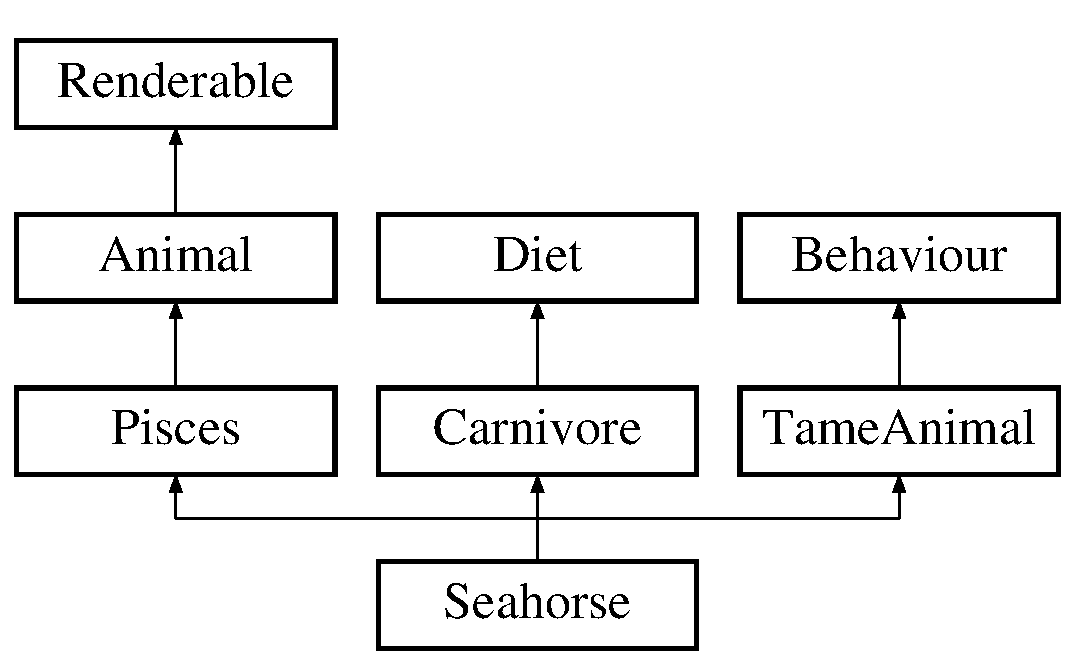
\includegraphics[height=4.000000cm]{classSeahorse}
\end{center}
\end{figure}
\subsection*{Public Member Functions}
\begin{DoxyCompactItemize}
\item 
\hypertarget{classSeahorse_ad2bd21fcd3f92b38833acd5951a0d843}{\hyperlink{classSeahorse_ad2bd21fcd3f92b38833acd5951a0d843}{Seahorse} (int \+\_\+weight)}\label{classSeahorse_ad2bd21fcd3f92b38833acd5951a0d843}

\begin{DoxyCompactList}\small\item\em Constructor. Menciptakan kuda laut. \end{DoxyCompactList}\item 
string \hyperlink{classSeahorse_ae08f997f9ffc0c9c0559dc355d58fa1a}{interact} () const 
\begin{DoxyCompactList}\small\item\em Melakukan interaksi dengan kuda laut. \end{DoxyCompactList}\end{DoxyCompactItemize}
\subsection*{Additional Inherited Members}


\subsection{Detailed Description}
Kelas \hyperlink{classSeahorse}{Seahorse} yang merepesentasikan kuda laut. 

\subsection{Member Function Documentation}
\hypertarget{classSeahorse_ae08f997f9ffc0c9c0559dc355d58fa1a}{\index{Seahorse@{Seahorse}!interact@{interact}}
\index{interact@{interact}!Seahorse@{Seahorse}}
\subsubsection[{interact}]{\setlength{\rightskip}{0pt plus 5cm}string Seahorse\+::interact (
\begin{DoxyParamCaption}
{}
\end{DoxyParamCaption}
) const}}\label{classSeahorse_ae08f997f9ffc0c9c0559dc355d58fa1a}


Melakukan interaksi dengan kuda laut. 

\begin{DoxyReturn}{Returns}
Experience yang dirasakan ketika berinteraksi dengan kuda laut. 
\end{DoxyReturn}


The documentation for this class was generated from the following files\+:\begin{DoxyCompactItemize}
\item 
src/\+Animal/\+Pisces/\+Seahorse/Seahorse.\+h\item 
src/\+Animal/\+Pisces/\+Seahorse/Seahorse.\+cpp\end{DoxyCompactItemize}

\hypertarget{classTameAnimal}{\section{Tame\+Animal Class Reference}
\label{classTameAnimal}\index{Tame\+Animal@{Tame\+Animal}}
}
Inheritance diagram for Tame\+Animal\+:\begin{figure}[H]
\begin{center}
\leavevmode
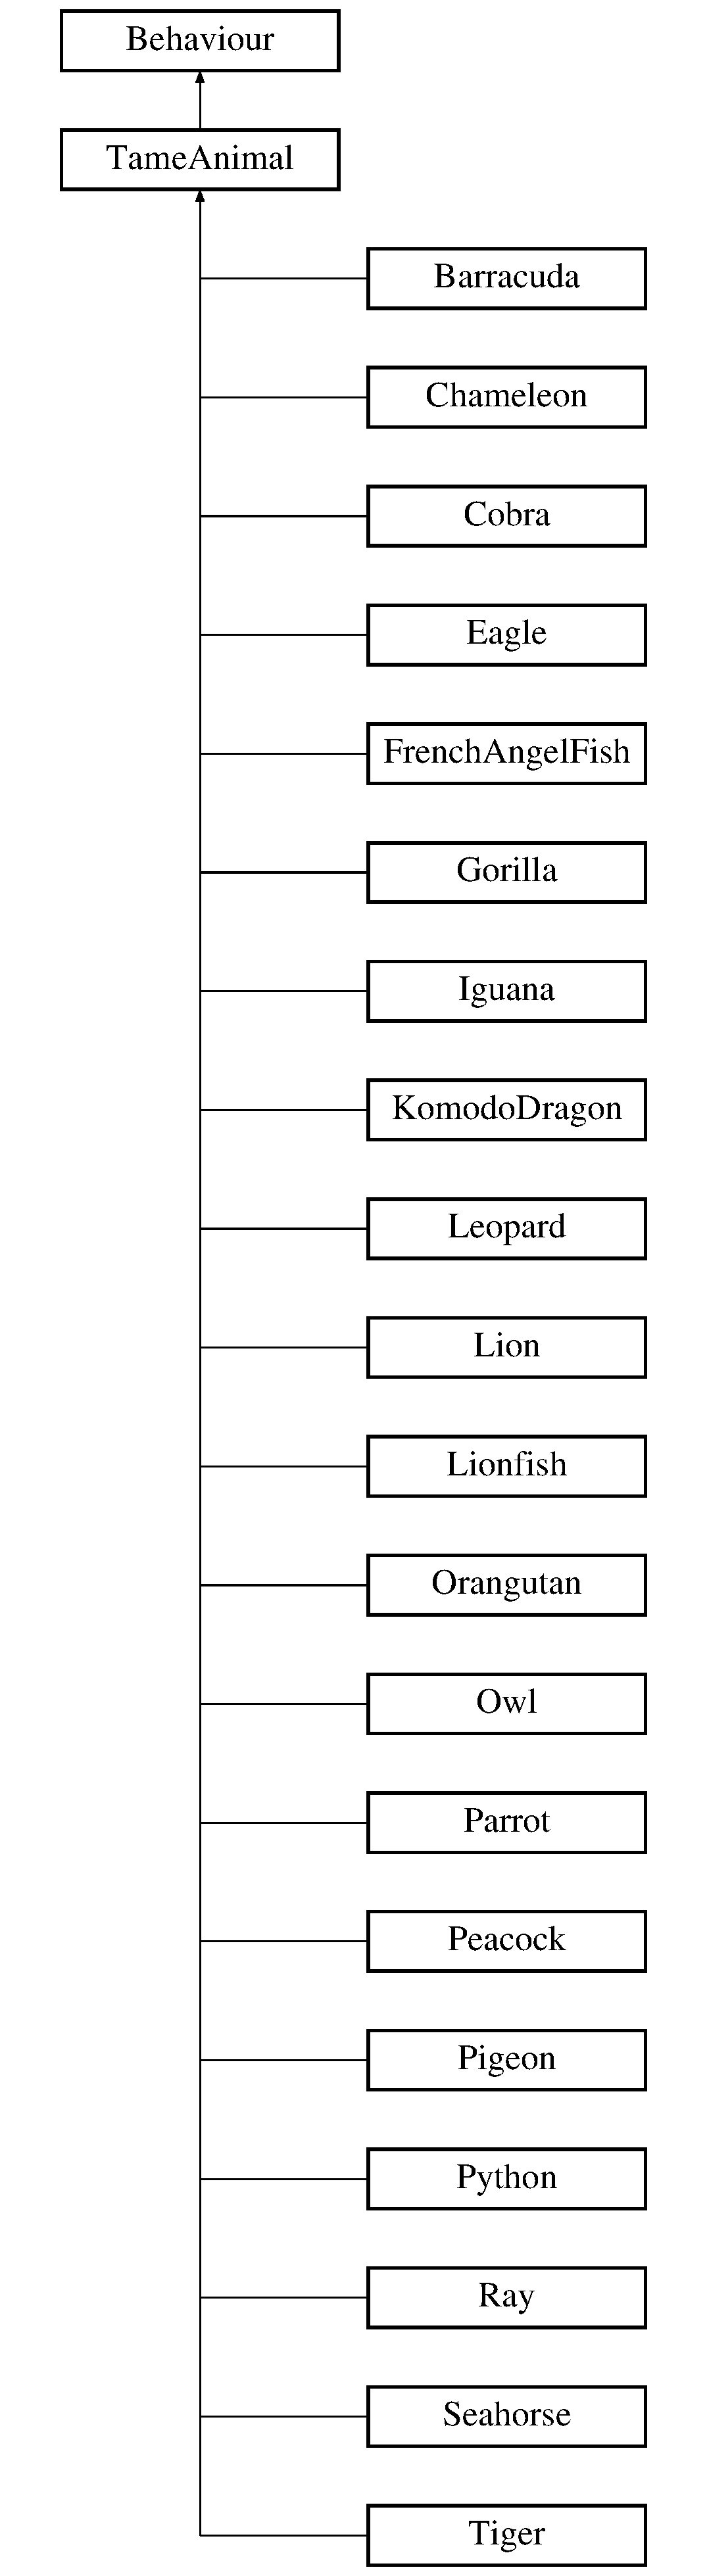
\includegraphics[height=12.000000cm]{classTameAnimal}
\end{center}
\end{figure}
\subsection*{Classes}
\begin{DoxyCompactItemize}
\item 
class \hyperlink{classTameAnimal_1_1Kelas}{Kelas}
\end{DoxyCompactItemize}
\subsection*{Public Member Functions}
\begin{DoxyCompactItemize}
\item 
\hypertarget{classTameAnimal_a8d8af9ffb8b945218e46aae2e0d7c1a7}{\hyperlink{classTameAnimal_a8d8af9ffb8b945218e46aae2e0d7c1a7}{Tame\+Animal} ()}\label{classTameAnimal_a8d8af9ffb8b945218e46aae2e0d7c1a7}

\begin{DoxyCompactList}\small\item\em Constructor. Menciptakan hewan jinak. \end{DoxyCompactList}\end{DoxyCompactItemize}
\subsection*{Additional Inherited Members}


The documentation for this class was generated from the following file\+:\begin{DoxyCompactItemize}
\item 
src/\+Animal/\+Behaviour/\+Tame\+Animal/Tame\+Animal.\+h\end{DoxyCompactItemize}

\hypertarget{classTiger}{\section{Tiger Class Reference}
\label{classTiger}\index{Tiger@{Tiger}}
}


{\ttfamily \#include $<$Tiger.\+h$>$}

Inheritance diagram for Tiger\+:\begin{figure}[H]
\begin{center}
\leavevmode
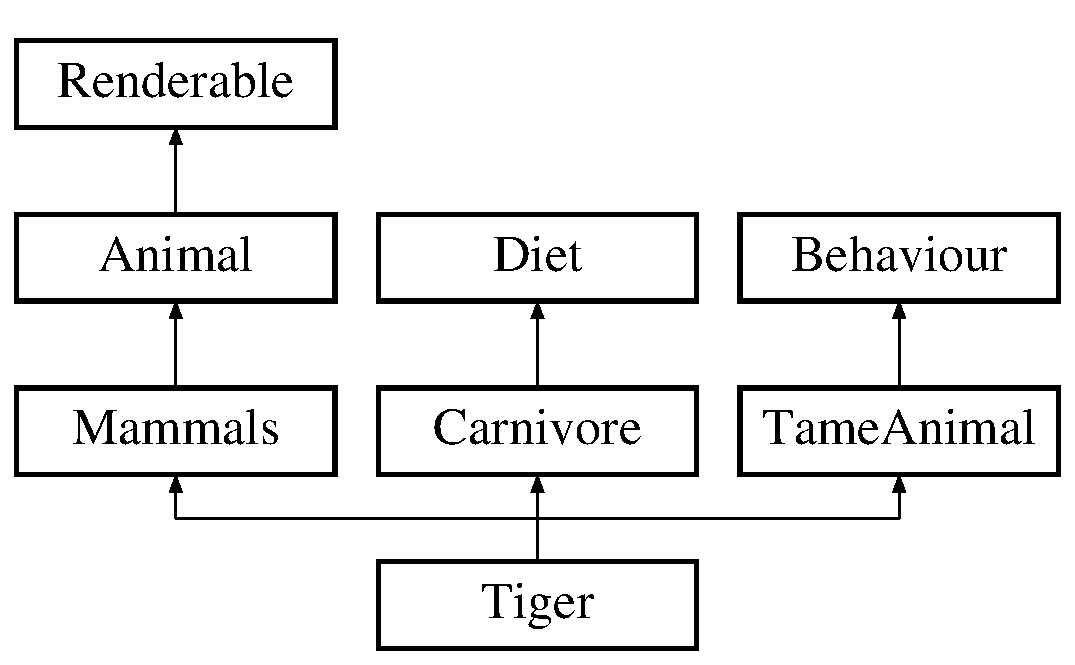
\includegraphics[height=4.000000cm]{classTiger}
\end{center}
\end{figure}
\subsection*{Public Member Functions}
\begin{DoxyCompactItemize}
\item 
\hypertarget{classTiger_a6b001b50f4e121add39d77e4dea2f0d8}{\hyperlink{classTiger_a6b001b50f4e121add39d77e4dea2f0d8}{Tiger} (int \+\_\+weight)}\label{classTiger_a6b001b50f4e121add39d77e4dea2f0d8}

\begin{DoxyCompactList}\small\item\em Constructor. Menciptakan harimau. \end{DoxyCompactList}\item 
string \hyperlink{classTiger_ac602680f7e8f50b4c1ca1892ce459a4e}{interact} () const 
\begin{DoxyCompactList}\small\item\em Melakukan interaksi dengan harimau. \end{DoxyCompactList}\end{DoxyCompactItemize}
\subsection*{Additional Inherited Members}


\subsection{Detailed Description}
Kelas \hyperlink{classTiger}{Tiger} yang merepesentasikan harimau. 

\subsection{Member Function Documentation}
\hypertarget{classTiger_ac602680f7e8f50b4c1ca1892ce459a4e}{\index{Tiger@{Tiger}!interact@{interact}}
\index{interact@{interact}!Tiger@{Tiger}}
\subsubsection[{interact}]{\setlength{\rightskip}{0pt plus 5cm}string Tiger\+::interact (
\begin{DoxyParamCaption}
{}
\end{DoxyParamCaption}
) const}}\label{classTiger_ac602680f7e8f50b4c1ca1892ce459a4e}


Melakukan interaksi dengan harimau. 

\begin{DoxyReturn}{Returns}
Experience yang dirasakan ketika berinteraksi dengan harimau. 
\end{DoxyReturn}


The documentation for this class was generated from the following files\+:\begin{DoxyCompactItemize}
\item 
src/\+Animal/\+Mammals/\+Tiger/Tiger.\+h\item 
src/\+Animal/\+Mammals/\+Tiger/Tiger.\+cpp\end{DoxyCompactItemize}

\hypertarget{classWaterHabitat}{\section{Water\+Habitat Class Reference}
\label{classWaterHabitat}\index{Water\+Habitat@{Water\+Habitat}}
}


{\ttfamily \#include $<$Water\+Habitat.\+h$>$}

Inheritance diagram for Water\+Habitat\+:\begin{figure}[H]
\begin{center}
\leavevmode
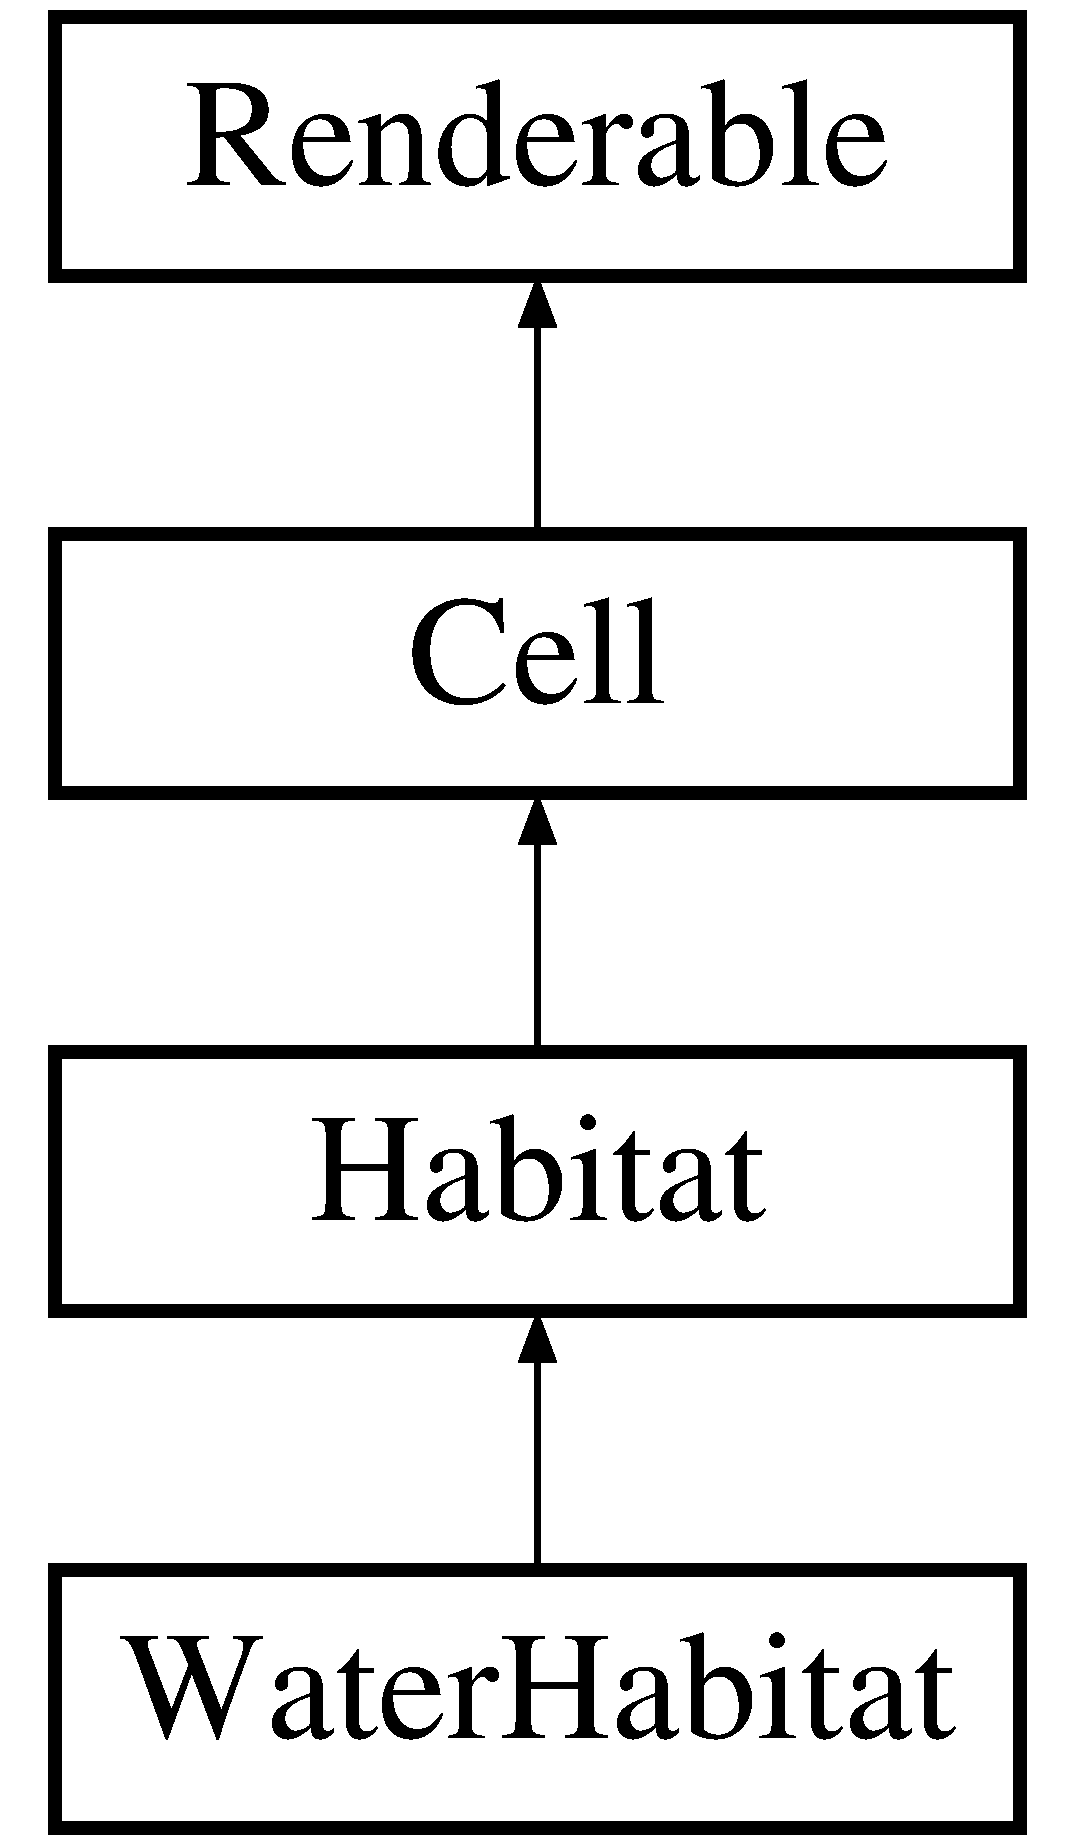
\includegraphics[height=4.000000cm]{classWaterHabitat}
\end{center}
\end{figure}
\subsection*{Public Member Functions}
\begin{DoxyCompactItemize}
\item 
\hypertarget{classWaterHabitat_a57a0d15fae5e17531835be2284df0fd1}{\hyperlink{classWaterHabitat_a57a0d15fae5e17531835be2284df0fd1}{Water\+Habitat} ()}\label{classWaterHabitat_a57a0d15fae5e17531835be2284df0fd1}

\begin{DoxyCompactList}\small\item\em Constructor. Menciptakan sebuah \hyperlink{classWaterHabitat}{Water\+Habitat}. \end{DoxyCompactList}\item 
\hypertarget{classWaterHabitat_abf6341b18b2fe62110998db3ffbde4b7}{virtual \hyperlink{classWaterHabitat_abf6341b18b2fe62110998db3ffbde4b7}{$\sim$\+Water\+Habitat} ()}\label{classWaterHabitat_abf6341b18b2fe62110998db3ffbde4b7}

\begin{DoxyCompactList}\small\item\em Destructor. \end{DoxyCompactList}\item 
\hypertarget{classWaterHabitat_a0820a384777ce7ba41244494e76eae13}{void \hyperlink{classWaterHabitat_a0820a384777ce7ba41244494e76eae13}{render} ()}\label{classWaterHabitat_a0820a384777ce7ba41244494e76eae13}

\begin{DoxyCompactList}\small\item\em Menampilkan \hyperlink{classWaterHabitat}{Water\+Habitat} ke console teks. \end{DoxyCompactList}\end{DoxyCompactItemize}
\subsection*{Additional Inherited Members}


\subsection{Detailed Description}
Kelas \hyperlink{classWaterHabitat}{Water\+Habitat} yang merepesentasikan habitat untuk hewan air. 

The documentation for this class was generated from the following files\+:\begin{DoxyCompactItemize}
\item 
src/\+Cell/\+Habitat/\+Water\+Habitat/Water\+Habitat.\+h\item 
src/\+Cell/\+Habitat/\+Water\+Habitat/Water\+Habitat.\+cpp\end{DoxyCompactItemize}

\hypertarget{classWildAnimal}{\section{Wild\+Animal Class Reference}
\label{classWildAnimal}\index{Wild\+Animal@{Wild\+Animal}}
}
Inheritance diagram for Wild\+Animal\+:\begin{figure}[H]
\begin{center}
\leavevmode
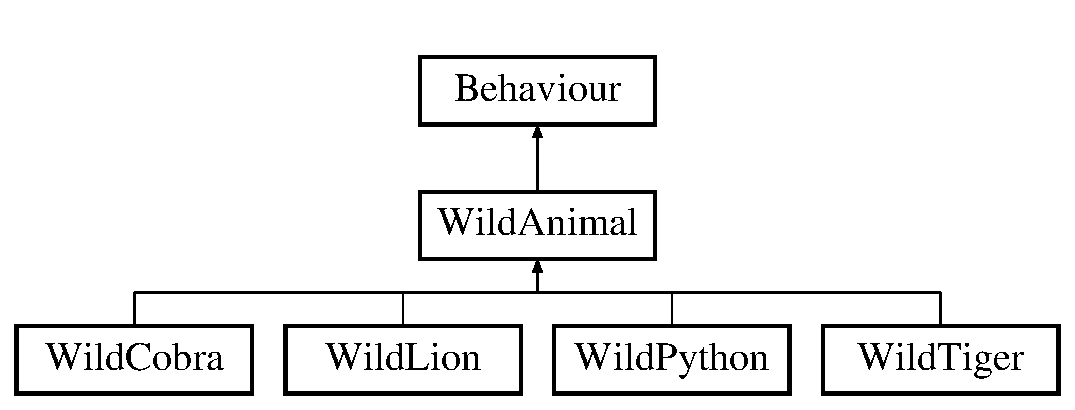
\includegraphics[height=3.000000cm]{classWildAnimal}
\end{center}
\end{figure}
\subsection*{Classes}
\begin{DoxyCompactItemize}
\item 
class \hyperlink{classWildAnimal_1_1Kelas}{Kelas}
\end{DoxyCompactItemize}
\subsection*{Public Member Functions}
\begin{DoxyCompactItemize}
\item 
\hypertarget{classWildAnimal_a3cdd77a1d03be27dc158981e71981384}{\hyperlink{classWildAnimal_a3cdd77a1d03be27dc158981e71981384}{Wild\+Animal} (int \+\_\+num\+Prey)}\label{classWildAnimal_a3cdd77a1d03be27dc158981e71981384}

\begin{DoxyCompactList}\small\item\em Constructor. Menciptakan hewan buas dengan jumlah mangsa tertentu. \end{DoxyCompactList}\item 
\hypertarget{classWildAnimal_a6ed385ed8a33fe29110ad7f4d05fb897}{\hyperlink{classWildAnimal_a6ed385ed8a33fe29110ad7f4d05fb897}{$\sim$\+Wild\+Animal} ()}\label{classWildAnimal_a6ed385ed8a33fe29110ad7f4d05fb897}

\begin{DoxyCompactList}\small\item\em Destructor. \end{DoxyCompactList}\item 
void \hyperlink{classWildAnimal_a3de85fd9006a69189b2c142cda11e5a2}{Add\+Prey} (const string \&prey\+Name)
\begin{DoxyCompactList}\small\item\em Menambahkan nama mangsa pada daftar mangsa. \end{DoxyCompactList}\item 
bool \hyperlink{classWildAnimal_a41475480d5e6b6ed07a18847e8cb5261}{is\+Prey} (const string \&prey\+Name) const 
\begin{DoxyCompactList}\small\item\em Memeriksa apakah prey\+Name terdapat pada prey\+List. \end{DoxyCompactList}\end{DoxyCompactItemize}
\subsection*{Protected Attributes}
\begin{DoxyCompactItemize}
\item 
\hypertarget{classWildAnimal_adcecee0efd159b656bcc03f3fbf0fa9e}{string $\ast$ {\bfseries prey\+List}}\label{classWildAnimal_adcecee0efd159b656bcc03f3fbf0fa9e}

\item 
\hypertarget{classWildAnimal_a3b941f33e34c5451eeabb452d6a095f9}{const int {\bfseries num\+Prey}}\label{classWildAnimal_a3b941f33e34c5451eeabb452d6a095f9}

\end{DoxyCompactItemize}


\subsection{Member Function Documentation}
\hypertarget{classWildAnimal_a3de85fd9006a69189b2c142cda11e5a2}{\index{Wild\+Animal@{Wild\+Animal}!Add\+Prey@{Add\+Prey}}
\index{Add\+Prey@{Add\+Prey}!Wild\+Animal@{Wild\+Animal}}
\subsubsection[{Add\+Prey}]{\setlength{\rightskip}{0pt plus 5cm}void Wild\+Animal\+::\+Add\+Prey (
\begin{DoxyParamCaption}
\item[{const string \&}]{prey\+Name}
\end{DoxyParamCaption}
)}}\label{classWildAnimal_a3de85fd9006a69189b2c142cda11e5a2}


Menambahkan nama mangsa pada daftar mangsa. 


\begin{DoxyParams}{Parameters}
{\em prey\+Name} & Nama mangsa. \\
\hline
\end{DoxyParams}
\hypertarget{classWildAnimal_a41475480d5e6b6ed07a18847e8cb5261}{\index{Wild\+Animal@{Wild\+Animal}!is\+Prey@{is\+Prey}}
\index{is\+Prey@{is\+Prey}!Wild\+Animal@{Wild\+Animal}}
\subsubsection[{is\+Prey}]{\setlength{\rightskip}{0pt plus 5cm}bool Wild\+Animal\+::is\+Prey (
\begin{DoxyParamCaption}
\item[{const string \&}]{prey\+Name}
\end{DoxyParamCaption}
) const}}\label{classWildAnimal_a41475480d5e6b6ed07a18847e8cb5261}


Memeriksa apakah prey\+Name terdapat pada prey\+List. 


\begin{DoxyParams}{Parameters}
{\em prey\+Name} & Nama mangsa. \\
\hline
\end{DoxyParams}
\begin{DoxyReturn}{Returns}
True jika prey\+Name terdapat pada prey\+List dan false jika tidak. 
\end{DoxyReturn}


The documentation for this class was generated from the following file\+:\begin{DoxyCompactItemize}
\item 
src/\+Animal/\+Behaviour/\+Wild\+Animal/Wild\+Animal.\+h\end{DoxyCompactItemize}

\hypertarget{classWildCobra}{\section{Wild\+Cobra Class Reference}
\label{classWildCobra}\index{Wild\+Cobra@{Wild\+Cobra}}
}


{\ttfamily \#include $<$Wild\+Cobra.\+h$>$}

Inheritance diagram for Wild\+Cobra\+:\begin{figure}[H]
\begin{center}
\leavevmode
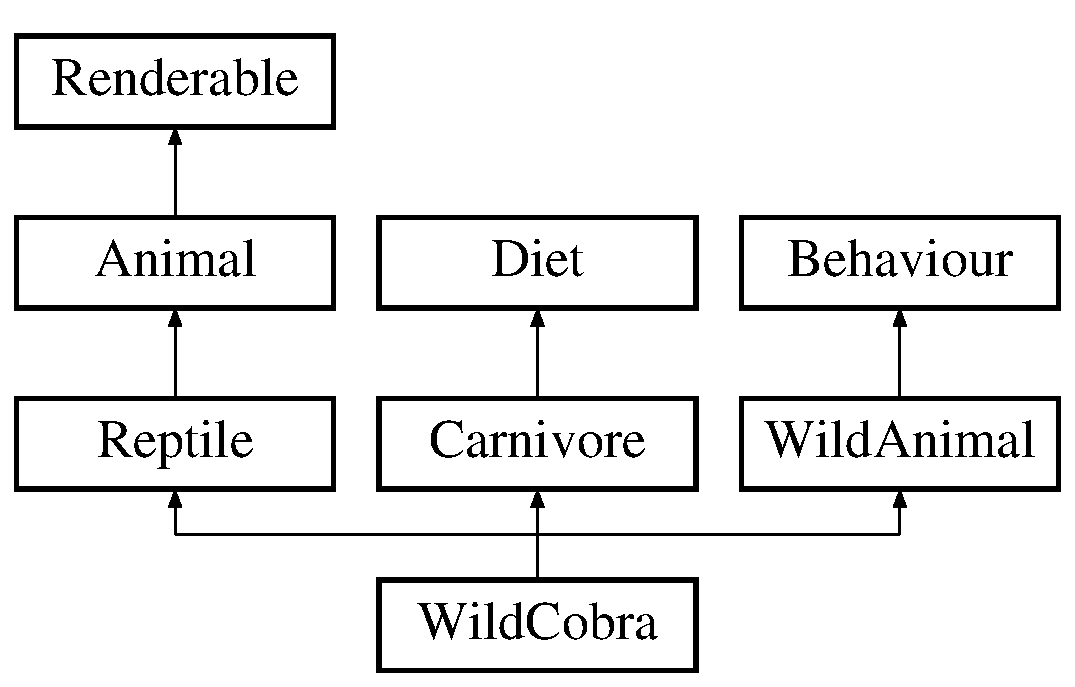
\includegraphics[height=4.000000cm]{classWildCobra}
\end{center}
\end{figure}
\subsection*{Public Member Functions}
\begin{DoxyCompactItemize}
\item 
\hypertarget{classWildCobra_a1a3170e5204edc488a88d2b1f26f8a5e}{\hyperlink{classWildCobra_a1a3170e5204edc488a88d2b1f26f8a5e}{Wild\+Cobra} (int \+\_\+weight)}\label{classWildCobra_a1a3170e5204edc488a88d2b1f26f8a5e}

\begin{DoxyCompactList}\small\item\em Constructor. Menciptakan ular kobra yang buas beserta daftar mangsanya. \end{DoxyCompactList}\item 
string \hyperlink{classWildCobra_ad1426b5e8ddc1ffbb830020623cb2a84}{interact} () const 
\begin{DoxyCompactList}\small\item\em Melakukan interaksi dengan ular kobra yang buas. \end{DoxyCompactList}\end{DoxyCompactItemize}
\subsection*{Additional Inherited Members}


\subsection{Detailed Description}
Kelas \hyperlink{classWildCobra}{Wild\+Cobra} yang merepesentasikan ular kobra yang buas. 

\subsection{Member Function Documentation}
\hypertarget{classWildCobra_ad1426b5e8ddc1ffbb830020623cb2a84}{\index{Wild\+Cobra@{Wild\+Cobra}!interact@{interact}}
\index{interact@{interact}!Wild\+Cobra@{Wild\+Cobra}}
\subsubsection[{interact}]{\setlength{\rightskip}{0pt plus 5cm}string Wild\+Cobra\+::interact (
\begin{DoxyParamCaption}
{}
\end{DoxyParamCaption}
) const}}\label{classWildCobra_ad1426b5e8ddc1ffbb830020623cb2a84}


Melakukan interaksi dengan ular kobra yang buas. 

\begin{DoxyReturn}{Returns}
Experience yang dirasakan ketika berinteraksi dengan ular kobra yang buas. 
\end{DoxyReturn}


The documentation for this class was generated from the following file\+:\begin{DoxyCompactItemize}
\item 
src/\+Animal/\+Reptile/\+Wild\+Cobra/Wild\+Cobra.\+h\end{DoxyCompactItemize}

\hypertarget{classWildLion}{\section{Wild\+Lion Class Reference}
\label{classWildLion}\index{Wild\+Lion@{Wild\+Lion}}
}


{\ttfamily \#include $<$Wild\+Lion.\+h$>$}

Inheritance diagram for Wild\+Lion\+:\begin{figure}[H]
\begin{center}
\leavevmode
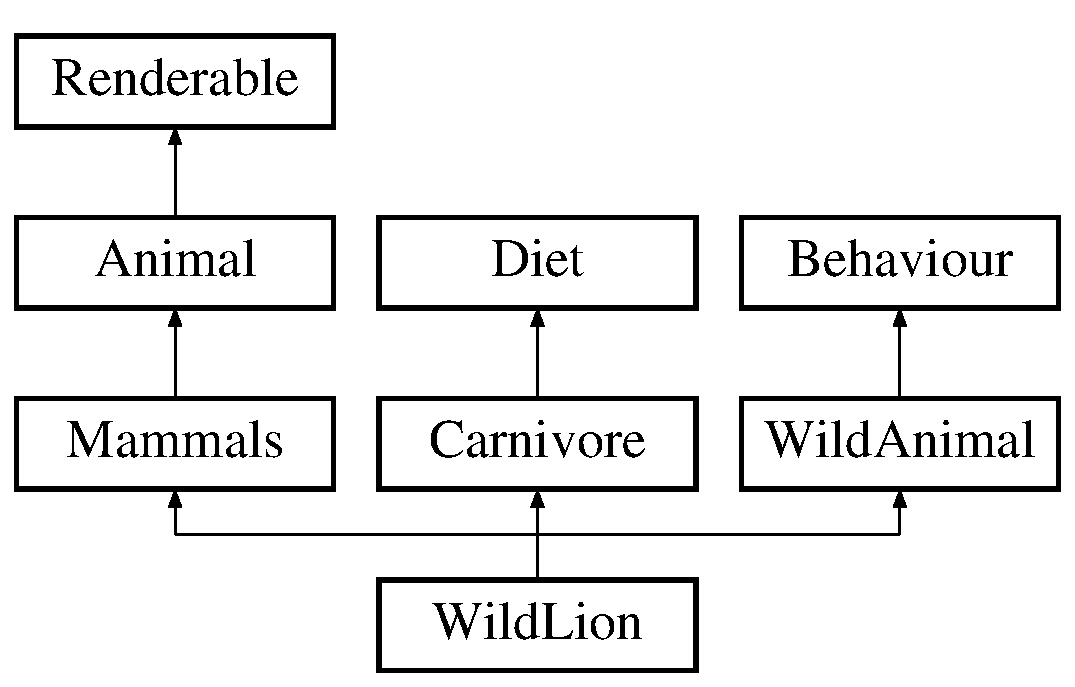
\includegraphics[height=4.000000cm]{classWildLion}
\end{center}
\end{figure}
\subsection*{Additional Inherited Members}


\subsection{Detailed Description}
Kelas \hyperlink{classWildLion}{Wild\+Lion} yang merepesentasikan singa yang buas. 

The documentation for this class was generated from the following file\+:\begin{DoxyCompactItemize}
\item 
src/\+Animal/\+Mammals/\+Wild\+Lion/Wild\+Lion.\+h\end{DoxyCompactItemize}

\hypertarget{classWildPython}{\section{Wild\+Python Class Reference}
\label{classWildPython}\index{Wild\+Python@{Wild\+Python}}
}


{\ttfamily \#include $<$Wild\+Python.\+h$>$}

Inheritance diagram for Wild\+Python\+:\begin{figure}[H]
\begin{center}
\leavevmode
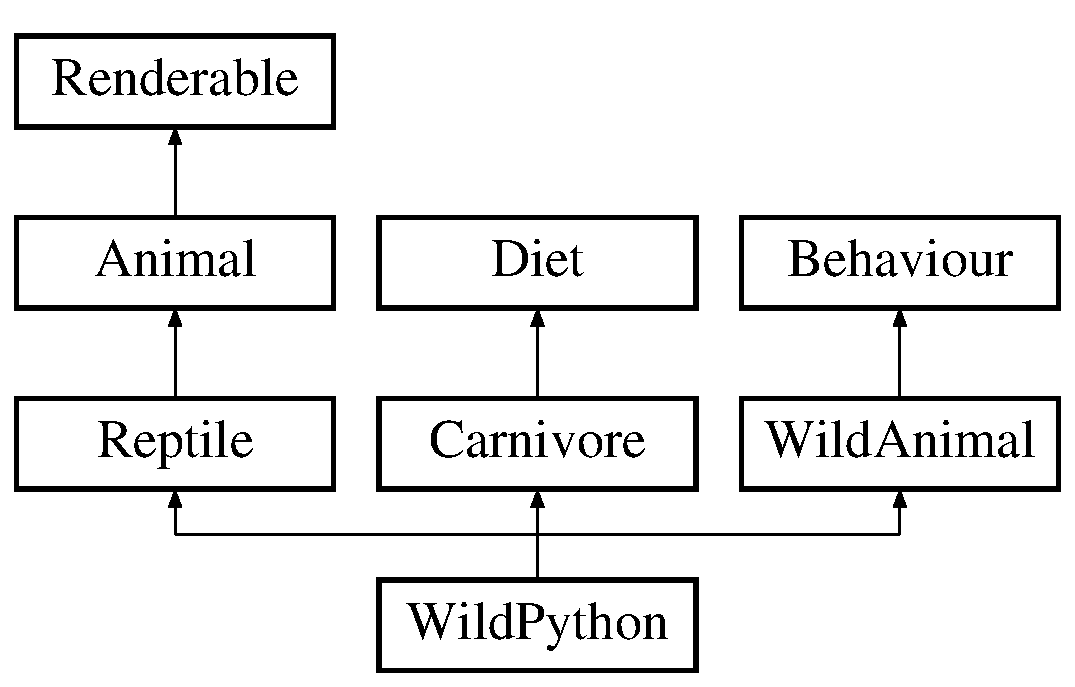
\includegraphics[height=4.000000cm]{classWildPython}
\end{center}
\end{figure}
\subsection*{Additional Inherited Members}


\subsection{Detailed Description}
Kelas \hyperlink{classWildPython}{Wild\+Python} yang merepesentasikan ular piton yang buas. 

The documentation for this class was generated from the following file\+:\begin{DoxyCompactItemize}
\item 
src/\+Animal/\+Reptile/\+Wild\+Python/Wild\+Python.\+h\end{DoxyCompactItemize}

\hypertarget{classWildTiger}{\section{Wild\+Tiger Class Reference}
\label{classWildTiger}\index{Wild\+Tiger@{Wild\+Tiger}}
}


{\ttfamily \#include $<$Wild\+Tiger.\+h$>$}

Inheritance diagram for Wild\+Tiger\+:\begin{figure}[H]
\begin{center}
\leavevmode
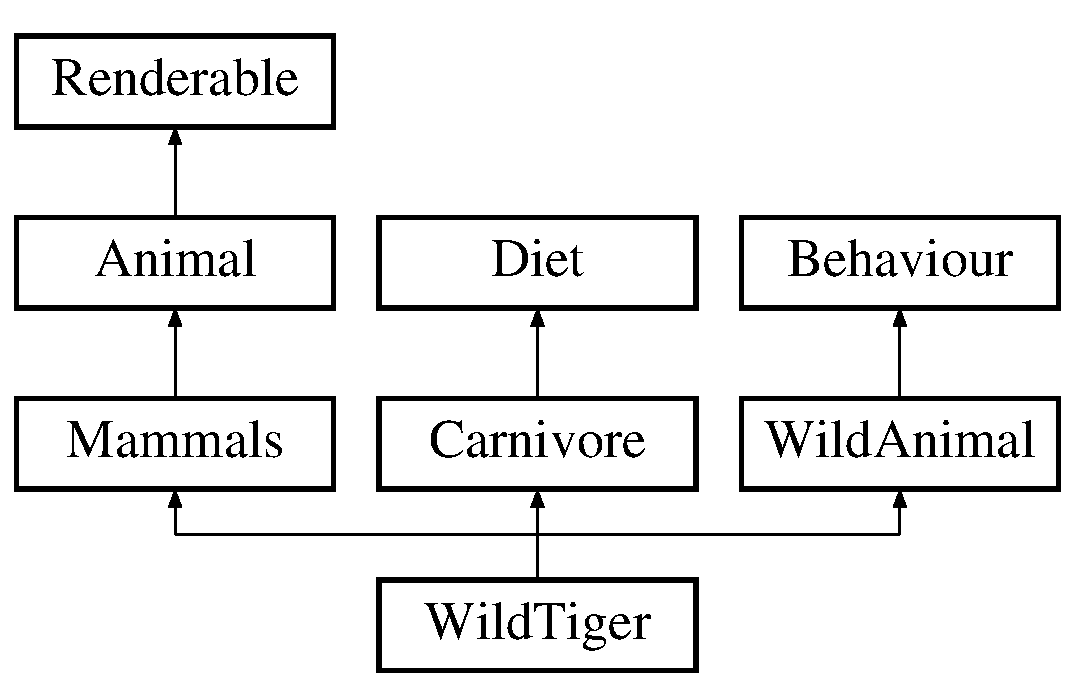
\includegraphics[height=4.000000cm]{classWildTiger}
\end{center}
\end{figure}
\subsection*{Additional Inherited Members}


\subsection{Detailed Description}
Kelas \hyperlink{classWildTiger}{Wild\+Tiger} yang merepesentasikan harimau yang buas. 

The documentation for this class was generated from the following file\+:\begin{DoxyCompactItemize}
\item 
src/\+Animal/\+Mammals/\+Wild\+Tiger/Wild\+Tiger.\+h\end{DoxyCompactItemize}

\hypertarget{classZoo}{\section{Zoo Class Reference}
\label{classZoo}\index{Zoo@{Zoo}}
}


{\ttfamily \#include $<$Zoo.\+h$>$}

\subsection*{Public Member Functions}
\begin{DoxyCompactItemize}
\item 
\hyperlink{classZoo_aaa0bf87b544fccd087e471ee0913709c}{Zoo} ()
\begin{DoxyCompactList}\small\item\em Constructor. \end{DoxyCompactList}\item 
\hypertarget{classZoo_a7a9114c178a5dc8f03a23911892015fb}{{\bfseries Zoo} (const \hyperlink{classZoo}{Zoo} \&)}\label{classZoo_a7a9114c178a5dc8f03a23911892015fb}

\end{DoxyCompactItemize}


\subsection{Detailed Description}
Kelas \hyperlink{classZoo}{Zoo} yang merepresentasikan sebuah kebun binatang. 

\subsection{Constructor \& Destructor Documentation}
\hypertarget{classZoo_aaa0bf87b544fccd087e471ee0913709c}{\index{Zoo@{Zoo}!Zoo@{Zoo}}
\index{Zoo@{Zoo}!Zoo@{Zoo}}
\subsubsection[{Zoo}]{\setlength{\rightskip}{0pt plus 5cm}Zoo\+::\+Zoo (
\begin{DoxyParamCaption}
{}
\end{DoxyParamCaption}
)}}\label{classZoo_aaa0bf87b544fccd087e471ee0913709c}


Constructor. 



The documentation for this class was generated from the following files\+:\begin{DoxyCompactItemize}
\item 
src/\+Zoo/Zoo.\+h\item 
src/\+Zoo/Zoo.\+cpp\end{DoxyCompactItemize}

%--- End generated contents ---

% Index
\newpage
\phantomsection
\addcontentsline{toc}{chapter}{Index}
\printindex

\end{document}
